%\documentclass[dissertation,draft]{softeng}
\documentclass[dissertation,final]{softeng}

\usepackage{ifdraft} % Contain macros to determine if document class has draft option or not

\usepackage{etoolbox}
\newtoggle{chapterone}
\newtoggle{chaptertwo}
\newtoggle{chapterthree}
\ifdraft
{
        \toggletrue{chapterthree}
        \toggletrue{chapterone}
        \toggletrue{chaptertwo}
}{
    \togglefalse{chapterthree}
    \togglefalse{chapterone}
    \togglefalse{chaptertwo}
}

% \togglefalse{workingmode}
% 


\usepackage{amsmath}
\usepackage{amsfonts}
\usepackage{amssymb}

\usepackage{times}
\usepackage{mathptmx}
\usepackage[utf8]{inputenc}

\usepackage[backend=biber,
            hyperref=false,
            natbib=true,
            citestyle=authoryear,
            bibstyle=authoryear-comp,
            url=false,
            isbn=false,
            doi=false,
            dashed=false,
            maxcitenames = 2, 
            mincitenames = 1, 
            maxbibnames = 3,
            firstinits = true,
            labelyear=true,  
            uniquename=false, 
            uniquelist=false,
            terseinits = false]{biblatex}

\addbibresource{mydissertation.bib}
\setlength\bibitemsep{1.5\itemsep}

\title{Extending BDD\\A systematic approach to handling non-functional requirements}
\author{Pedro Moreira}
\college{Kellogg College}
\organisation{University of Oxford}
\award{Software Engineering}

\usepackage[english, status=draft]{fixme}
\fxusetheme{color}

\usepackage{xspace}
\newcommand{\nfrs}{non-functional requirements\xspace}
\newcommand{\Nfrs}{Non-functional requirements\xspace}

\usepackage[english]{babel}
\usepackage[autostyle=true,english=british]{csquotes}
\SetCiteCommand{\citep}


\usepackage{pgfplotstable}
\usepackage{booktabs}
\usepackage{array}
\usepackage{colortbl}
\usepackage{tabularx}
\usepackage{rotating}
\usepackage{graphicx} %package to manage images
\graphicspath{ {Images/} {Images/case_study/} }

\colorlet{tableheadcolor}{gray!25} % Table header colour = 25% gray
\newcommand{\headcol}{\rowcolor{tableheadcolor} \bfseries} %he
\colorlet{tablerowcolor}{gray!10} % Table row separator colour = 10% gray
\newcommand{\rowcol}{\rowcolor{tablerowcolor}} %
    % Command \midline consists of 3 rules (top colour tableheadcolor, middle colour black, bottom colour white)
\newcommand{\midline}{
            \arrayrulecolor{tableheadcolor}\specialrule{\aboverulesep}{-1pt}{0pt}%
            \arrayrulecolor{black}\specialrule{\lightrulewidth}{0pt}{0pt}%
            \arrayrulecolor{white}\specialrule{\belowrulesep}{0pt}{-3pt}%
            \arrayrulecolor{black}
            }
\usepackage{multirow}
            
\uchyph=0 % Prevent hyphenation of all uppercase words (normally acronyms)

\usepackage[outputdir=Temp,newfloat=true,cache=false]{minted}
\setminted[gherkin]{frame=lines,
                    framesep=2mm,
                    fontsize=\footnotesize,
                    baselinestretch=1.2,
                    samepage=true,
                    stripnl=false,
                    obeytabs=false,
                    tabsize=4}
\usemintedstyle{bw}
\SetupFloatingEnvironment{listing}{name=Source Code / Feature}
\SetupFloatingEnvironment{listing}{listname=List of Source Code / Feature}

% Used for Listings of Features
\newsavebox{\featurebox} 
\newenvironment{featurecode}[1]
{ \lrbox\featurebox \begin{adjustbox}{width=#1\textwidth,minipage=\textwidth,center} }
{ \end{adjustbox}\endlrbox}

\newenvironment{featurelist}[2]
{
\newcommand{\setcaption}{\caption{#1}}
\newcommand{\setlabel}{\label{#2}}
}
{\begin{listing}[h!]\centering\usebox\featurebox\setcaption\setlabel\end{listing}}

\usepackage{caption}

\usepackage{adjustbox}

\usepackage{relsize} % Package for font resizing

\usepackage[toc,page]{appendix} % package to add appendixes and list them in table of contents

\usepackage{longtable}  % As the name says, supports tables that span multiple pages

%\renewcommand\listoflistingscaption{List of source code}
%\renewcommand{\listingscaption}{Source code}

\setcounter{LTchunksize}{50}

\begin{document}

\maketitle


\begin{abstract}
Software engineering methods have evolved from having a prescribed and sequential nature to using more adaptable and iterative approaches. Such is the case with Behaviour Driven Development (BDD), a recent member of the family of agile methodologies addressing the correct specification of the behaviour characteristics of a system, by focusing on close collaboration and identification of examples.

Whilst BDD is very successful in ensuring developed software meets its functional requirements, it is largely silent regarding the systematic treatment of its non-functional counterparts, descriptions of how the system should behave with respect to some quality attribute such as performance, reusability, etc.

Historically, the systematic treatment of non-functional requirements (NFRs) in software engineering is categorised as being either product-oriented and based on a quantitative approach aimed at evaluating the degree to which a system meets its NFRs or process-oriented, qualitative in nature and where they are used to drive the software design process. Examples of the latter category, are the NFR Framework -- a structured approach to represent and reason about non-functional requirements -- and the goal-oriented requirements language (GRL) that provides support for evaluation and analysis of the most appropriate trade-offs among (often conflicting) goals of stakeholders. 

In this thesis, we investigate the extent to which goal-oriented principles can be integrated in BDD, with the aim of handling non-functional requirements in an explicit and systematic way, whilst respecting the principles and philosophy behind agile development.
\end{abstract}

\clearpage

\begin{acknowledgements}
  \ifdraft{%
    \fxnote{THIS WILL acknoeledgements}
  }{%
  I would like to express my deepest gratitude to my supervisor, Dr Jeremy Gibbons, for his guidance, support, comments and encouragement.
  
  I would also like to thank my family for their constant support and love, and in particular my wife, Tamara and my children Elijah and Indigo, for their endless patience whenever I so often disappeared into the office to research and write this thesis.
  
  My sincere thanks to my mother who always encouraged and supported me through my studies and, more importantly, through all my life.
  
  \emph{The author confirms that}: this dissertation does not contain material previously submitted for another degree or academic award; and the work presented here is the author's own, except where otherwise stated.
  }
\end{acknowledgements}


\pagenumbering{roman}
\pagestyle{plain}
\setcounter{tocdepth}{2}

\tableofcontents

\listoffigures
\listoftables
\listoflistings

\pagenumbering{arabic}
\pagestyle{myheadings}

\chapter{Introduction}
\label{ch:Introduction}
\iftoggle{chapterone}
{
    \fxnote{Chapter one will go here}
}
{
This thesis presents an extension to Behaviour Driven Development~(BDD)~\citep{North2006,Smart201410} to support the elicitation, communication, modelling and analysis of non-functional requirements. It includes concepts and techniques from goal-oriented requirements engineering (GORE)~\citep{Lamsweerde:2001wpba}, and more specifically, allows the definition of goals in BDD and modelling and analysis in Goal Requirements Language (GRL)~\citep{Amyot2010}. This is achieved by integrating notions of goals in Gherkin~\citep{wynne2012cucumber} -- a domain specific language for the representation and specification of requirements. We also present a translator from Gherkin to GRL, allowing Gherkin-defined actors and goals satisfactions levels to be subject to qualitative and quantitative analysis in a GRL tool.

\section{Motivation}
The primary measure of success of a software system is the degree to which it meets the purpose for which it was intended~\citep{Nuseibeh:2000ub}. Shortcomings in the ways that people learn about, document, agree upon and modify such statements of intent are known causes to many of the problems in software development~\citep{Wiegers2013}. We informally refer to these statements of intent as Requirements and the engineering process to elicit, document, verify, validate and manage them as Requirements Engineering~\footnote{These topics will be explored in depth in Chapter~\ref{ch:Background}}.

The importance of requirements in software engineering cannot be understated. In his essay \emph{No Silver Bullet},~\citet{Brooks1987}, referring to the critical role of requirements to a software project, states that 
\blockcquote{Brooks1987}{The hardest single part of building a software system is deciding precisely what to build. No other part of the conceptual work is as difficult as establishing the detailed technical requirements, including all the interfaces to people, to machines, and to other software systems. No other part of the work so cripples the resulting system if done wrong. No other part is more difficult to rectify later.}

 More recently, ~\citet{Davis200505} reveals that errors introduced during requirements activities account for 40 to 50 percent of all defects found in a software product.  When arguing for the importance of requirements, \citet{Hull2011} reason that to be well understood by everybody they are generally expressed in natural language and herein lies the challenge: to capture the need or problem completely and unambiguously without resorting to specialist jargon or conventions. The authors follow by positing these needs may not be clearly defined at the start, may conflict or be constrained by factors outside their control or may be influenced by other goals which themselves change in the course of time.

Furthermore, requirements can be classified in multiple and at times conflicting ways. \citet{Glinz:2007ehba} points out that in every current classification scheme there is a distinction between requirements concerning the functionality of a system and all other, often referred to as non-functional requirements. In another paper, the same author points out issues with current classification schemes such as sub-classification, terminology and satisfaction level whereby some requirements are considered \emph{`soft'} in the sense that they can be weakly or strongly satisfied (e.g \emph{the system shall have a good performance}; or \emph{the System shall be secure}). \citet{Chung:2009vg} contribute that, in spite of this separation, most existing requirement models and requirements specification languages lack a proper treatment of non-functional requirements. In addition, this separation of functional and non-functional requirements has lead to the latter being either neglected, addressed later in a project or completely ignored. This problem applies to both traditional and agile software development processes. 

A software process is generically defined as a set of activities, methods, practices, and transformations that are used to develop and maintain software and its associated products~\citep{Cugola:1998htba}. Agile software development approaches have become more popular during the last few years. Several methods have been developed with the aim of delivering software faster and to ensure that the software meets customer changing needs. All these approaches share some common principles: Improved customer satisfaction, adopting requirements, frequently to changing delivering working software, and close collaboration of business people and developers~\citep{Paetsch:2003tl}.

One of such agile approaches is Behaviour Driven Development (BDD). The understanding of BDD is far from clear and unanimous~\citep{Solis0}. Some authors refer to BDD as a development process~\citep{Smart201410}, others state that it is not a fully fledged software development methodology but rather \emph{\textcquote{Adzic201106}{supplement other methodologies, provide rigour in specifications and testing, enhance communication between various stakeholders and members of software development teams, reduce unnecessary rework, and facilitate change.}}

In spite of the above mentioned differences of interpretation, it is unanimously accepted that BDD focus on deriving from  business goals, a sufficiently set of software features that contribute to achieve these business goals. This process makes use of Gherkin~\citep{wynne2012cucumber} -- a domain specific language which promotes the use of a ubiquitous language~\footnote{~Eric Evans first introduced that term in \citetitle{evans2004domain} \citet{evans2004domain}}  that business people can understand -- to describe and model a system. However the focus has been on functionality and quality characteristics such as performance, security, maintainability are not explicitly addressed. To the best of our knowledge, the single exception to the above, is the work of \citet{barmi2011automated}, but with restricted applicability to probabilistic -- those that can be written using probabilistic statements~\citep{grunske2008specification} -- non-functional requirements only.

None of these agile practices, treat non-functional requirements in a systematic way, certainly not in a way that allows reasoning about which requirements interdependencies may exist, and the positive or negative influences each may have on each other. Among many proposals, goal-oriented approaches were the first to treat non-functional requirements as first-class citizens.~\citet{Mylopoulos:1999jh} observed that goal-oriented requirements engineering is generally complementary to other approaches and, in particular, is well suited to analysing requirements early in the software development cycle, especially with respect to non-functional requirements and the evaluation of alternatives. 

It seems only logical and expectable that, improvements to the discovery and communication of requirements, and in particular non-functional requirements, will lead to an increase in success rates of software projects.

\section{Aim and limitations of study}
The context described in the previous section justify research aimed at capturing, documenting and communicating requirements using natural language tools and techniques in a precise, complete and unambiguous way, but also with the flexibility and adaptability to allow requirements to change and evolve through the course of time.

In this thesis, we investigate the extent to which goal-oriented principles can be integrated in BDD, with the aim of handling non-functional requirements in an explicit and systematic way, whilst respecting the principles and philosophy behind agile development. In particular, we consider how BDD can be extended, and also Gherkin modified, to incorporate actor and goal concepts as defined and treated in GRL.

We do not however investigate the integration of GRL with use case maps (UCM), as part of the User Requirements Notation~\citep{liu2004designing}. UCM targets modelling scenarios of functional or operational requirements and performance and architectural reasoning. This is left as an area for further research.

We also do not aim at providing another classification scheme and address the, sometimes artificial, separation of functional and non-functional requirements. Instead, we adopt the notion of goals as an objective the system under consideration should achieve and goals formulations as properties to be ensured. We share the view that goals cover different types of concerns: functional which are associated with the services to be provided, and non-functional concerns associated with quality of service such as safety, security, accuracy, performance, and so forth~\citep{Lamsweerde:2001wpba}.

Finally, we do not apply this technique to a specific non-functional requirement or restrict the validity of our results to any particular taxonomy, as our approach is independent of the NFR being addressed or taxonomy chosen.

\section{Significance of the study}

By reinterpreting behaviours in BDD as not just specifications of functionality of a system but as statements of goals, this thesis brings the following contributions to BDD:

\begin{center}
\begin{itemize}
\item Allows non-functional requirements to be specified in natural language form in Gherkin
\item Allows Gherkin specifications to be converted into goal models and imported and used in jUCMNav
\item Allows BDD to consider all non-functional requirements, not just those that are technical, but still relevant for a successful product delivery
\item Brings to BDD the capability to assess qualitative and quantitative satisfaction levels of actors and goals 
\end{itemize}
\end{center}

By allowing goals to be elicited and specified in Gherkin, this thesis brings the following contributions to goal-oriented requirements engineering:

\begin{center}
\begin{itemize}
\item Allows goals elicitation to occur in Gherkin using natural language and therefore more suitable for discussion and fostering communication
\item Brings the benefits of executable specifications in BDD to goal formulations
\end{itemize}
\end{center}


\section{Overview of contents}

We have now reviewed the motivation for this study, stated the aim of the research and identified the contributions our work brings to BDD and goal-oriented requirements engineering and the research community in general. The rest of the thesis is organised as follows:

Chapter~\ref{ch:Background} contains all the necessary background material related to requirements engineering, the approaches taken by agile processes and, in particular section~\ref{ch:Background:sec:bdd} on behaviour-driven development, describing the principles and practices of this popular agile process. Chapter~\ref{ch:nfr_research} presents an overview of the research concerning ways of handling non-functional requirements in software engineering and section~\ref{sec:gore} on goal-oriented requirements engineering with a focus on GRL and with a description of jUCMNav~\citep{Amyot2010}, an editor for GRL models.

Chapter~\ref{ch:Extendingbdd} and chapter~\ref{ch:gherkin_redux} are the core of the thesis and contain details of extensions to Gherkin; mapping of Gherkin elements to GRL, such as actors and intentional elements and a description of a translator from Gherkin to an XML-based interchange format to be used in jUCMNav.

Chapter~\ref{ch:Extendingbdd} focus more on the practical uses of the extended methodology, while chapter~\ref{ch:gherkin_redux} exposes the technical details of the implementation changes made to Gherkin and introduces a translator from Gherkin to GRL.

Chapter~\ref{ch:Conclusion} contains implications of findings, concluding thoughts, identifies limitations of study and suggests topics for future research.
}
\chapter{From traditional to agile requirements engineering}
\label{ch:Background}
In Chapter~\ref{ch:Introduction} we have outlined and situated our study around insufficiencies in current approaches to handling non-functional requirements in agile development methods, and behaviour-driven development in particular. 

In this chapter, we reflect on how fast-changing technology and increased competition are placing an ever increasing pressure on the development process. We first review the notions of requirements and requirements engineering, highlighting the most used processes and activities, regardless of the software development method in use. We follow with a description of requirements engineering practices in agile methods and finish with a presentation of key concepts of behaviour-driven development (BDD), contextualising BDD as an instance of \emph{Specification by Example}~\citep{Adzic201106}.

\section{Requirements}
\label{sec:requirements}
Despite decades of industry experience, many software organizations struggle to understand, document, and manage their product requirements. Inadequate user input, incomplete requirements, changing requirements, and misunderstood business objectives are major reasons why so many information technology projects are less than fully successful. Some software teams lack the proficiency of eliciting requirements from customers and other sources. Customers often don't have the time or patience to participate in requirements activities~\citep{Wiegers2013}. 

Effective requirements engineering is crucial to delivering products and services aligned to the goals and objectives for which they were initially conceived. \citet{Hull2011} state that software is the most powerful force behind changes of new products and is mostly driven by three factors: \emph{arbitrary complexity}, due to most products having software at its core and being often complex; \emph{instant distribution} -- new products or changes to existing products can be distributed to its clients in a matter of seconds or minutes, usually the time it takes to download, install and configure a new software version -- and \emph{off-the-shelf components}, as most systems can now be built from ready-made components, greatly reducing the product development cycle.

\subsection{Definition}
Many problems in the software world arise from shortcomings in the ways that people learn about, document, agree upon and modify product's requirements. Common problem areas are informal information gathering, implied functionality, miscommunicated assumptions, poorly specified requirements, and a casual change process~\citep{Wiegers2013}. Various studies suggest that errors introduced during requirements activities account for 40 to 50 percent of all defects found in a software product~\citep{Davis200505}. Inadequate user input and shortcomings in specifying and managing customer requirements are major contributors to unsuccessful projects. Despite this evidence, many organizations still practice ineffective requirements methods. There is no definitive definition of requirements that satisfies all purposes and concerns, but the ones we provide next, are some of the more consensual ones~\citep{Wiegers2013}.

The difficulty with defining requirements, arises mostly due to a terminology problem. Different observers might describe a single statement as being a user requirement, software requirement, business requirement, functional requirement, system requirement, product requirement, project requirement, user story, feature, or constraint~\citep{Wiegers2013}. Because of the inter-connectedness of requirements with other aspects of systems engineering and project management, it is quite challenging to find a satisfactory scope for a definition of requirements engineering~\citep{Hull2011}. A typical definition of requirement can be found in ~\citefield{ieee_std_29148}{journaltitle}
\begin{displayquote}
A statement that identifies a product or process operational, functional, or design characteristic or constraint, which is unambiguous, testable or measurable, and necessary for product or process acceptability (by consumers or internal quality assurance guidelines)
\end{displayquote}
It is worth breaking down this definition into its constituents words. A requirement comes mostly in a textual representation~(\emph{statement}) even though there are other complementary or alternative forms such visual forms, formal methods and domain specific languages. Requirements may define what is to be built in response to requirements~(\emph{product requirements}) but also procedures for using what will be built~(\emph{process requirements}). In addition, there may be requirements that stipulate how the product should be developed, usually for quality control purposes. The definition also allures for the existence of many different kinds of requirements, such as \emph{operational, functional, or design characteristic or constraint}, giving rise to different kinds of language, analysis, modelling, process and solution. It states that a requirement should lend itself to a clear, single understanding, common to all parties involved~(\emph{unambiguous}). It should also be quantifiable, thus providing a means of measuring and testing the solution against it. Finally, requirements play a multi-dimensional role and come from a multitude of sources. \citet{Sommerville:1997} shares a simpler, but nevertheless, useful definition
\begin{displayquote}
Requirements are a specification of what should be implemented. They are descriptions of how the system should behave, or of a system property or attribute. They may be a constraint on the development process of the system.
\end{displayquote}
This definition makes clear that different types of information are part of requirements domain. Requirements mean different things for different people: for users, they represent external characteristics of the system behaviour, whilst for developers, they are instead linked with internal characteristics. They include both the behaviour of the system under specific conditions and those properties that make it suitable -- and maybe even enjoyable -- for use by its intended users~\citep{Wiegers2013}.

\subsection{Classification}

\citet{Wiegers2013} provide a breakdown of different types of information that may be categorised as requirements. Given that the term `requirement' is extremely overloaded in software engineering, it is useful to give definitions of these information types, and contextualise their use and relevance (see table~\ref{tb:typesofreqs}). 

\ifdraft{%
  \fxnote{This will contain a table of REquirements Information}
}{%
\begin{table}[h!]
\caption[Types of requirements information]{Types of requirements information~\citep{Wiegers2013}}
\label{tb:typesofreqs}
\setlength{\extrarowheight}{1.8pt}
\centering
\scalebox{0.75}{
\begin{tabularx}{\textwidth}{cX}
\toprule \multicolumn{1}{c}{\bfseries{Term}}&
\multicolumn{1}{c}{\bfseries{Definition}}\\
\addlinespace
\midrule
Business requirement & A high-level business objective of the organization that builds a product or of a customer who procures it\\ \midrule
Business rule &   A policy, guideline, standard, or regulation that defines or constrains some aspect of the business. Not a software requirement in itself, but the origin of several types of software requirements \\ \midrule
Constraint &    A restriction that is imposed on the choices available to the developer for the design and construction of a product \\ \midrule
External interface requirement &   A description of a connection between a software system and a user, another software system, or a hardware device \\ \midrule
Feature &    One or more logically related system capabilities that provide value to a user and are described by a set of functional requirements \\ \midrule
Functional requirement &    A description of a behaviour that a system will exhibit under specific conditions \\ \midrule
Non-functional requirement &  A description of a property or characteristic that a system must exhibit or a constraint that it must respect \\ \midrule
Quality attribute &    A kind of nonfunctional requirement that describes a service or performance characteristic of a product \\ \midrule
System requirement &    A top-level requirement for a product that contains multiple subsystems, which could be all software or software and hardware \\ \midrule
User requirement &    A goal or task that specific classes of users must be able to perform with a system, or a desired product attribute \\
\addlinespace
\bottomrule
\end{tabularx}
}
\end{table}
}
\emph{Business requirements} describe why the organization is implementing the system and the business benefits the organization hopes to achieve. The focus is on the business objectives of the organization or the customer who requests the system. Business requirements typically come from the funding sponsor for a project, the acquiring customer, the manager of the actual users, the marketing department, or a product visionary. Business requirements are usually contained within a vision and scope document. Other strategic guiding documents sometimes used for this purpose include a project charter, business case, and market (or marketing)~\mbox{requirements} document~\citep{Wiegers2013}.

\emph{User requirements} describe goals or tasks the users must be able to perform with the product that will provide value to someone. The domain of user requirements also includes descriptions of product attributes or characteristics that are important to user satisfaction. Ways to represent user requirements include use cases~\citep{cockburn2000writing}, user stories~\citep{cohn2004user}, and event-response tables. Ideally, actual user representatives will provide this information. User requirements describe what the user will be able to do with the system. Some people use the broader term `stakeholder requirements' to acknowledge the reality that various stakeholders other than direct users will provide requirements. A good set of stakeholder requirements can provide a concise non-technical description of what is being developed at a level that is accessible to senior management.

\emph{Functional requirements} specify the behaviours the product will exhibit under specific conditions. They describe what the developers must implement to enable users to accomplish their tasks (user requirements), thereby satisfying the business requirements. These are usually documented in a software requirements specification (SRS), which describes as fully as necessary the expected behaviour of the software system. The SRS is used in development, testing, quality assurance, project management, and related project functions. People call this deliverable by many different names, including business requirements document, functional spec, requirements document, and others.

\emph{System requirements} describe the requirements for a product that is composed of multiple components or subsystems. A `system' in this sense, is not just any information system. A system can be all software or it can include both, software and hardware subsystems. People and processes are part of a system too, so certain system functions might be allocated to human beings. The system requirements can form an excellent technical summary of a development project~\citep{Hull2011}.

\emph{Business rules} include corporate policies, government regulations, industry standards, and computational algorithms. Business rules are not themselves software requirements because they have an existence beyond the boundaries of any specific software application. However, they often dictate that the system must contain functionality to comply with the pertinent rules. Sometimes, as with corporate security policies, business rules are the origin of specific quality attributes that are then implemented in functionality. Therefore, you can trace the genesis of certain functional requirements back to a particular business rule.

In addition to functional requirements, the SRS contains an assortment of \emph{non-functional requirements}. \emph{Quality attributes} are also known as quality factors, quality of service requirements, constraints, and the `-ilities'. They describe the product's characteristics in various dimensions that are important either to users or to developers and maintainers, such as performance, safety, availability, and portability. Other classes of non-functional requirements describe \emph{external interfaces} between the system and the outside world. These include connections to other software systems, hardware components, and users, as well as communication interfaces. Design and implementation \emph{constraints} impose restrictions on the options available to the developer during construction of the product.

Figure~\ref{fig:types_of_requirements} depicts the relationships among these types of requirements information, using ovals for requirements and rectangles for documents. In the figure, solid arrows mean `are stored in'; dotted arrows mean `are the origin of' or `influence'.
\begin{figure}[h!]
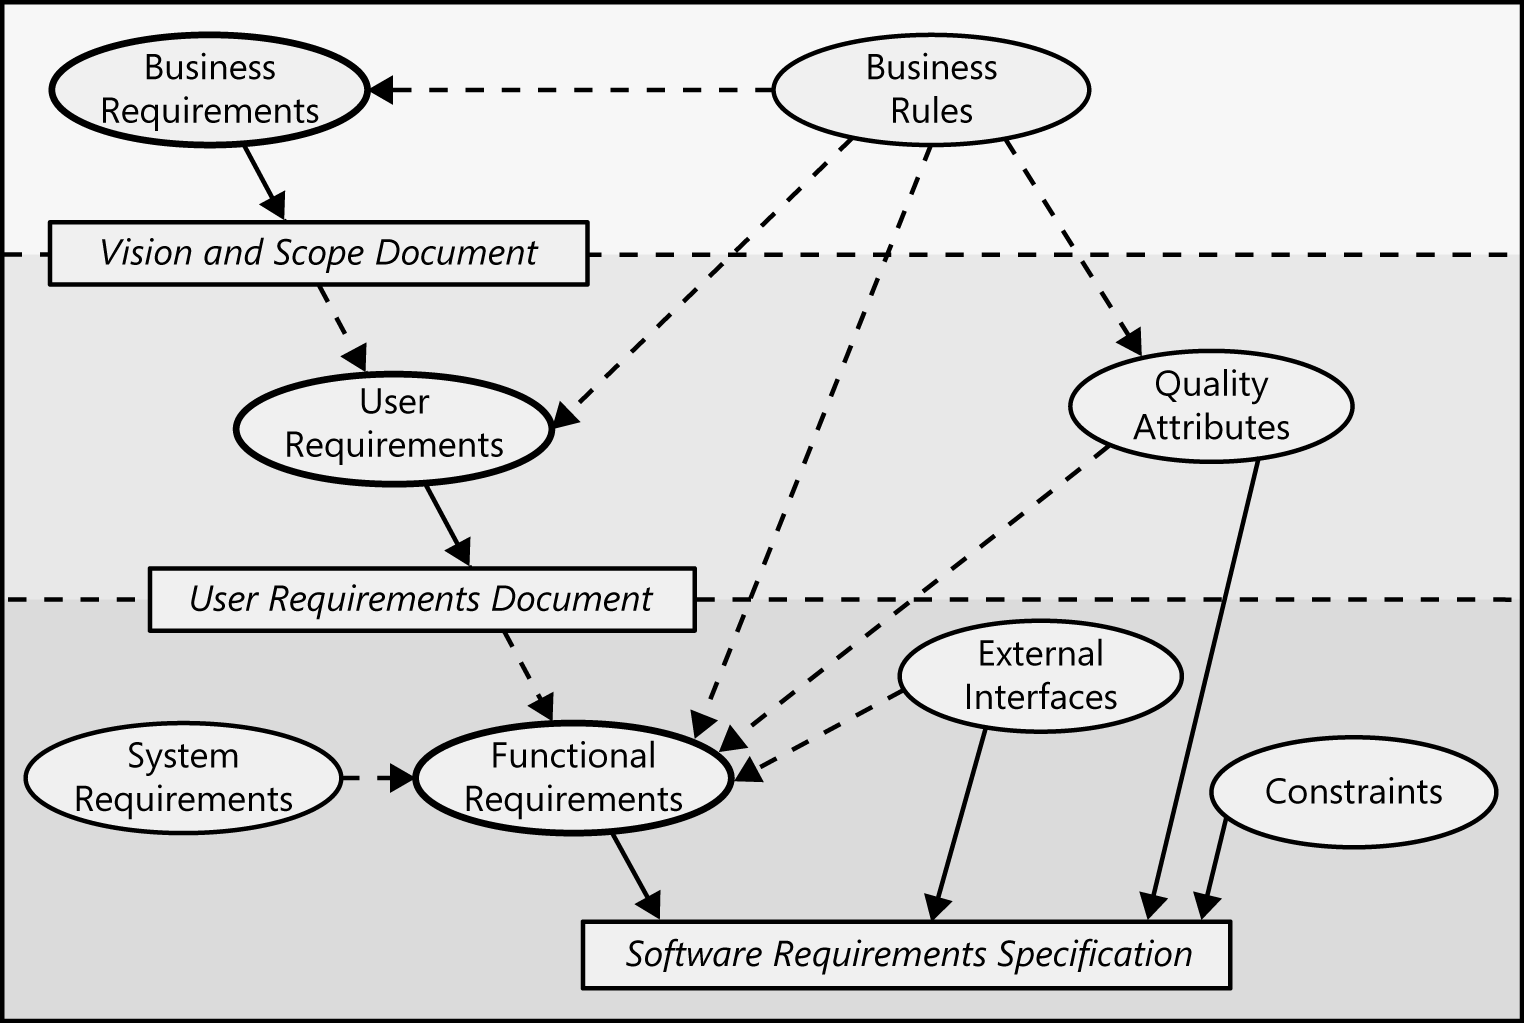
\includegraphics[width=0.75\textwidth]{TypesOfRequirements}
\centering
\caption[Types of Requirements]{Relationships among several types of requirements information~\citep[p. 8]{Wiegers2013}}
\label{fig:types_of_requirements}
\end{figure}

A \emph{feature} consists of one or more logically related system capabilities that provide value to a user, and are described by a set of functional requirements. A feature can encompass multiple user requirements, each of which implies that certain functional requirements must be implemented to allow the user to perform the task described by each user requirement. %Figure~\ref{fig:feature_tree} illustrates a feature tree, an analysis model that shows how a feature can be hierarchically decomposed into a set of smaller features, which relate to specific user requirements and lead to specifying sets of functional requirements.
%
%\begin{figure}[h!]
%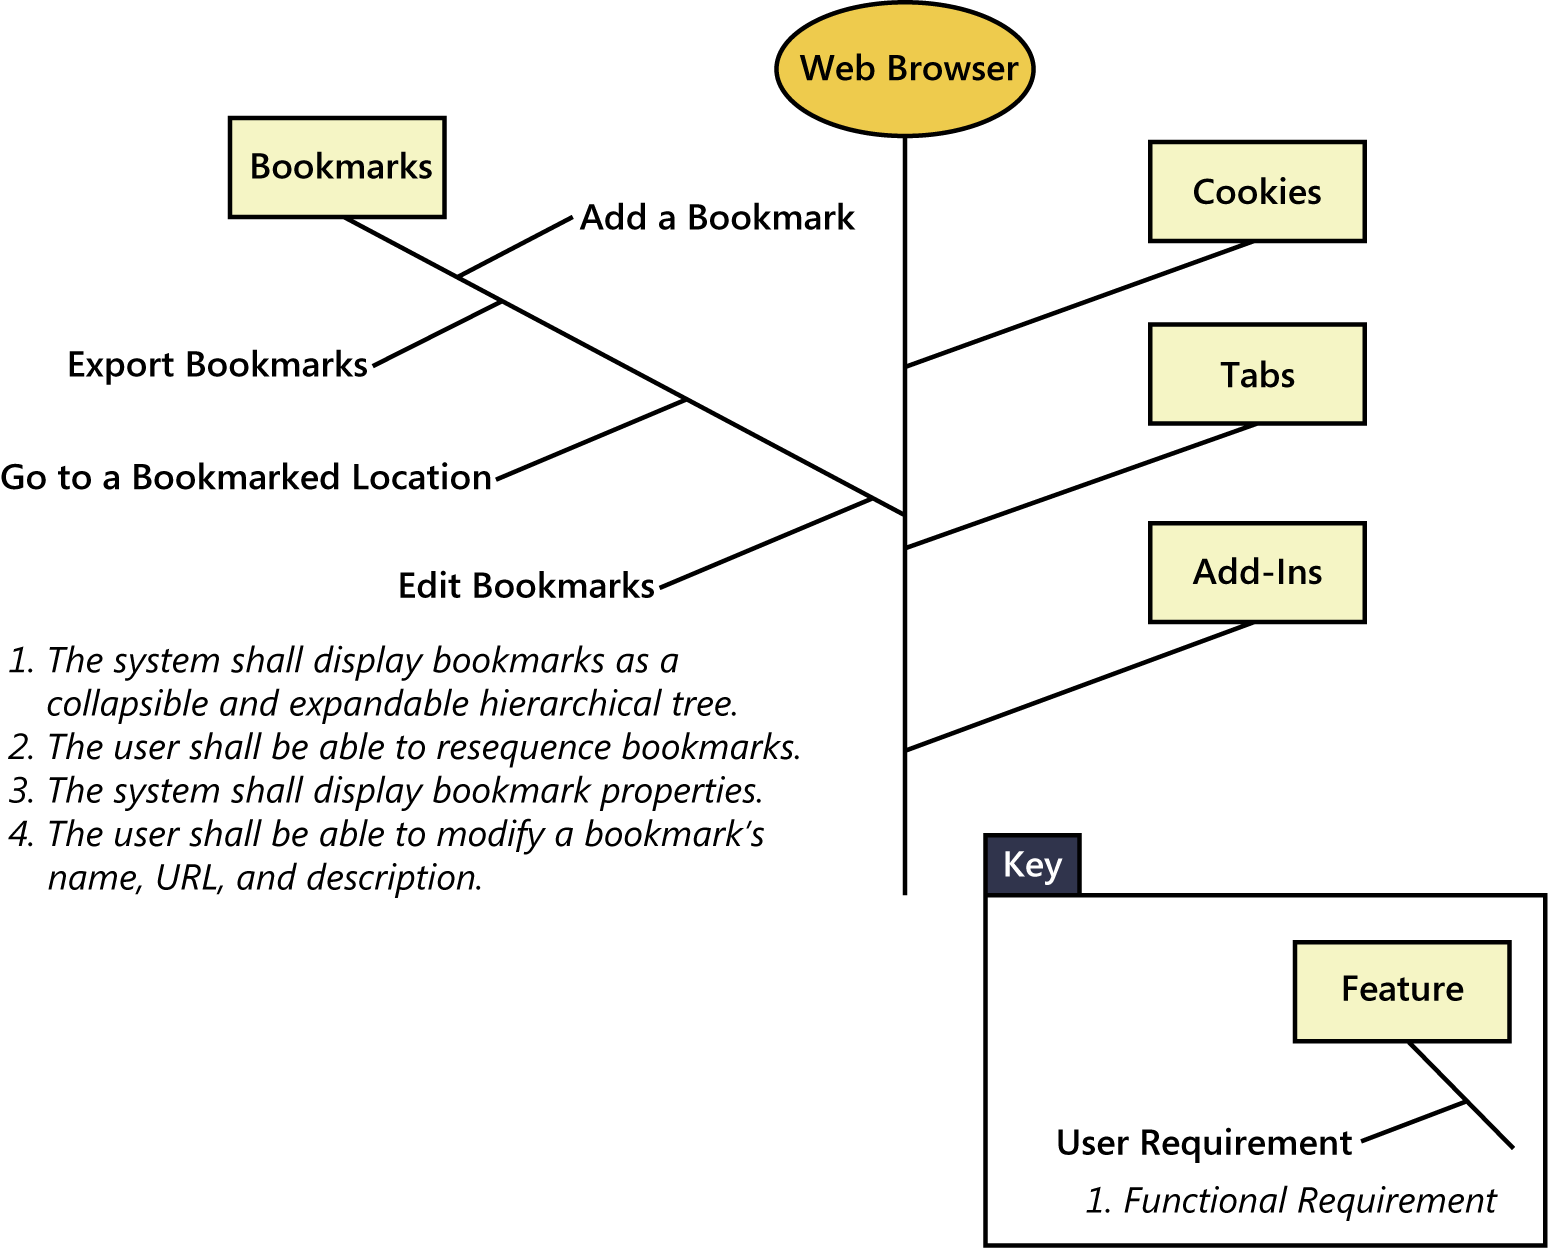
\includegraphics[width=0.75\textwidth]{FeatureTree}
%\centering
%\caption[Feature Trees]{Relationships among features, user requirements, and functional requirements~\citep[p. 11]{Wiegers2013}}
%\label{fig:feature_tree}
%\end{figure}

We have identified three major requirements deliverables: a vision and scope document, a user requirements document, and a software requirements specification. There is often no need to create three discrete requirements deliverables on each project. It often makes sense to combine some of this information, particularly on small projects. However, we should recognize that these three deliverables contain different information, are developed at different points in the project, possibly by different people and with different purposes and target audiences~\citep{Wiegers2013}.

Requirements can also be categorised as either \emph{product} or \emph{project} requirements. Product requirements are those that describe properties of a software system to be built. Projects certainly do have other expectations and deliverables that are not a part of the software the team implements, but that are necessary to the successful completion of the project as a whole. These are project requirements but not product requirements. An SRS houses the product requirements, but it should not include design or implementation details (other than known constraints), project or test plans, or similar information.

\citet{Hull2011} make an important distinction between requirements being defined in either a \emph{problem} or \emph{solution} domain. In the context of requirements existing at different layers of abstraction, those at higher layers, representative of statements of need, usage modelling and stakeholder requirements, pertain to the problem domain, whereas those in lower layers, starting with system requirements, operate in the solution domain. The use of multiple levels of abstraction promotes separation of concerns and allows views of stakeholders, analysts and developers to be taken in consideration. Stakeholder requirements should specify only what they want to achieve and avoid any reference to particular solutions. System requirements, on the other hand, should abstractly specify what the system will do to meet the stakeholder requirements, whilst avoiding any references to any particular design. Finally, subsystem and component requirements, part of architectural designs, will specify how this design meets the system requirements.


\section{Requirements Engineering}
\label{sec:requirements_eng}
The \emph{\citefield{SWEBOK}{maintitle}}~(\citetitle{SWEBOK}, \citeyear{SWEBOK}) identifies topics that pertain to software requirements knowledge, which concern the elicitation, analysis, specification, and validation of software requirements as well as their management during the whole life cycle of a software product.

%\begin{figure}[h]
%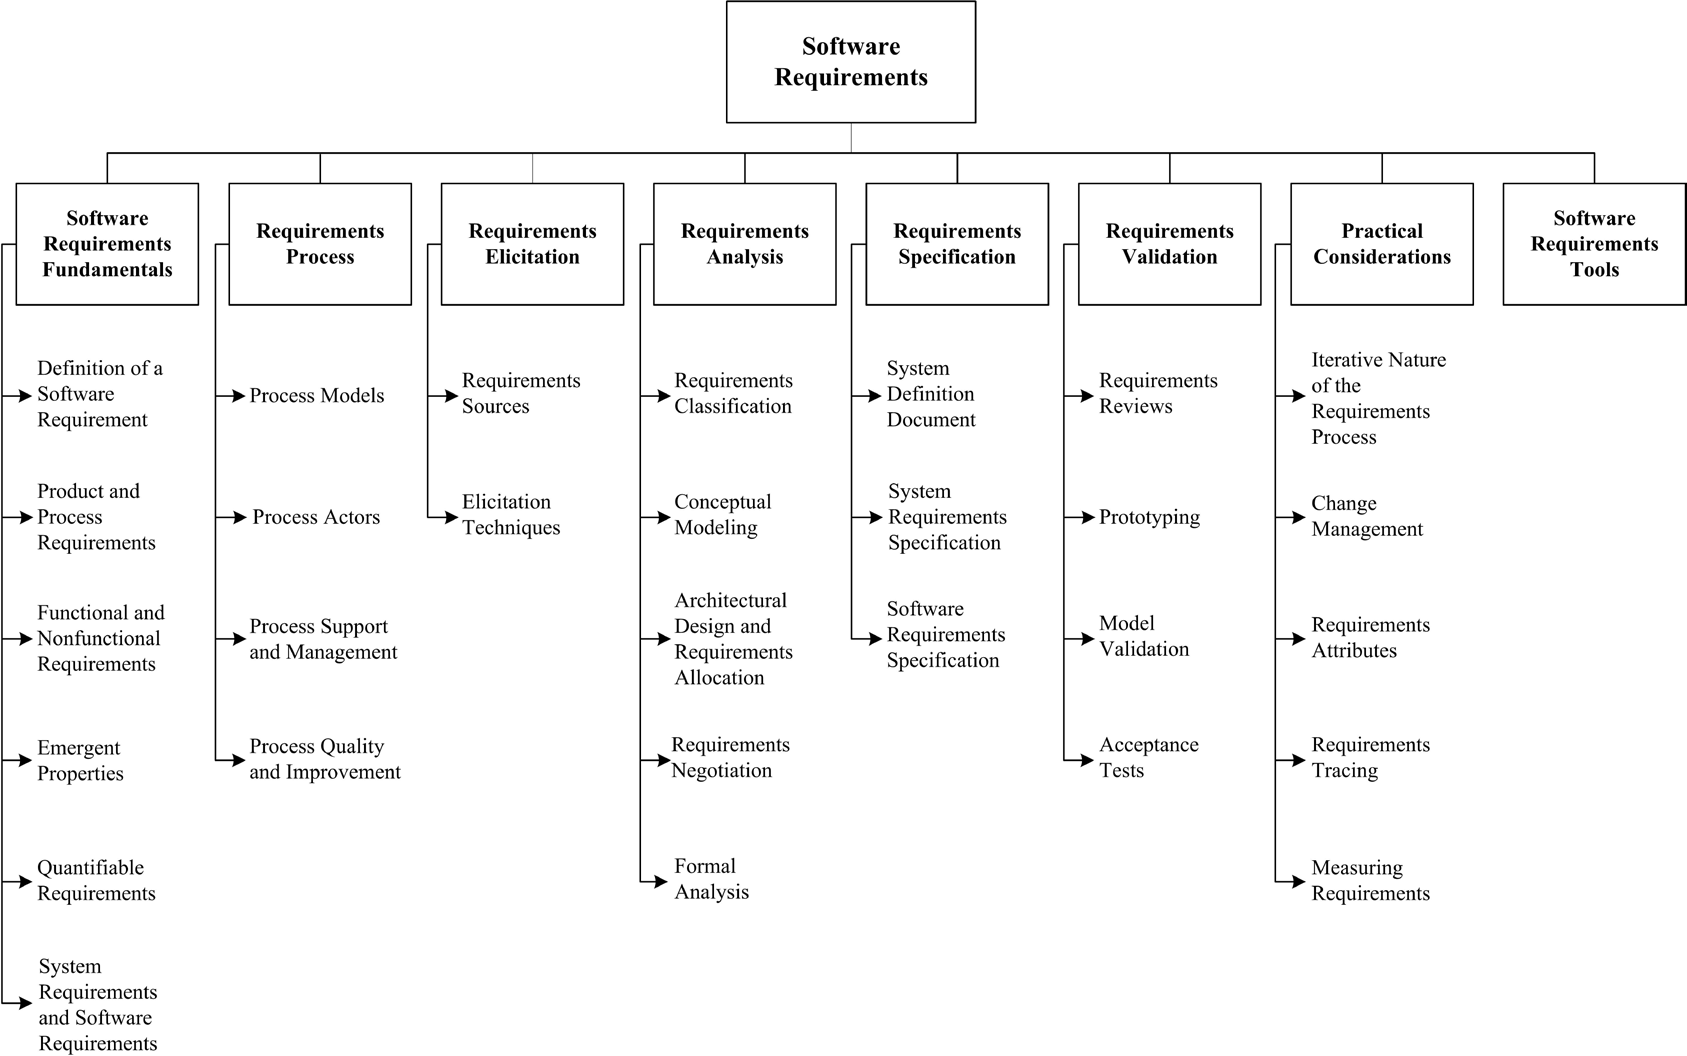
\includegraphics[width=0.9\textwidth]{swebooksoftwarerequirements}
%\centering
%\caption[Topics for software requirements]{Topics for the Software Requirements knowledge area~(\citetitle{SWEBOK}, \citeyear{SWEBOK})}
%\label{fig:swebook_software_requirements}
%\end{figure}

\begin{sidewaysfigure}
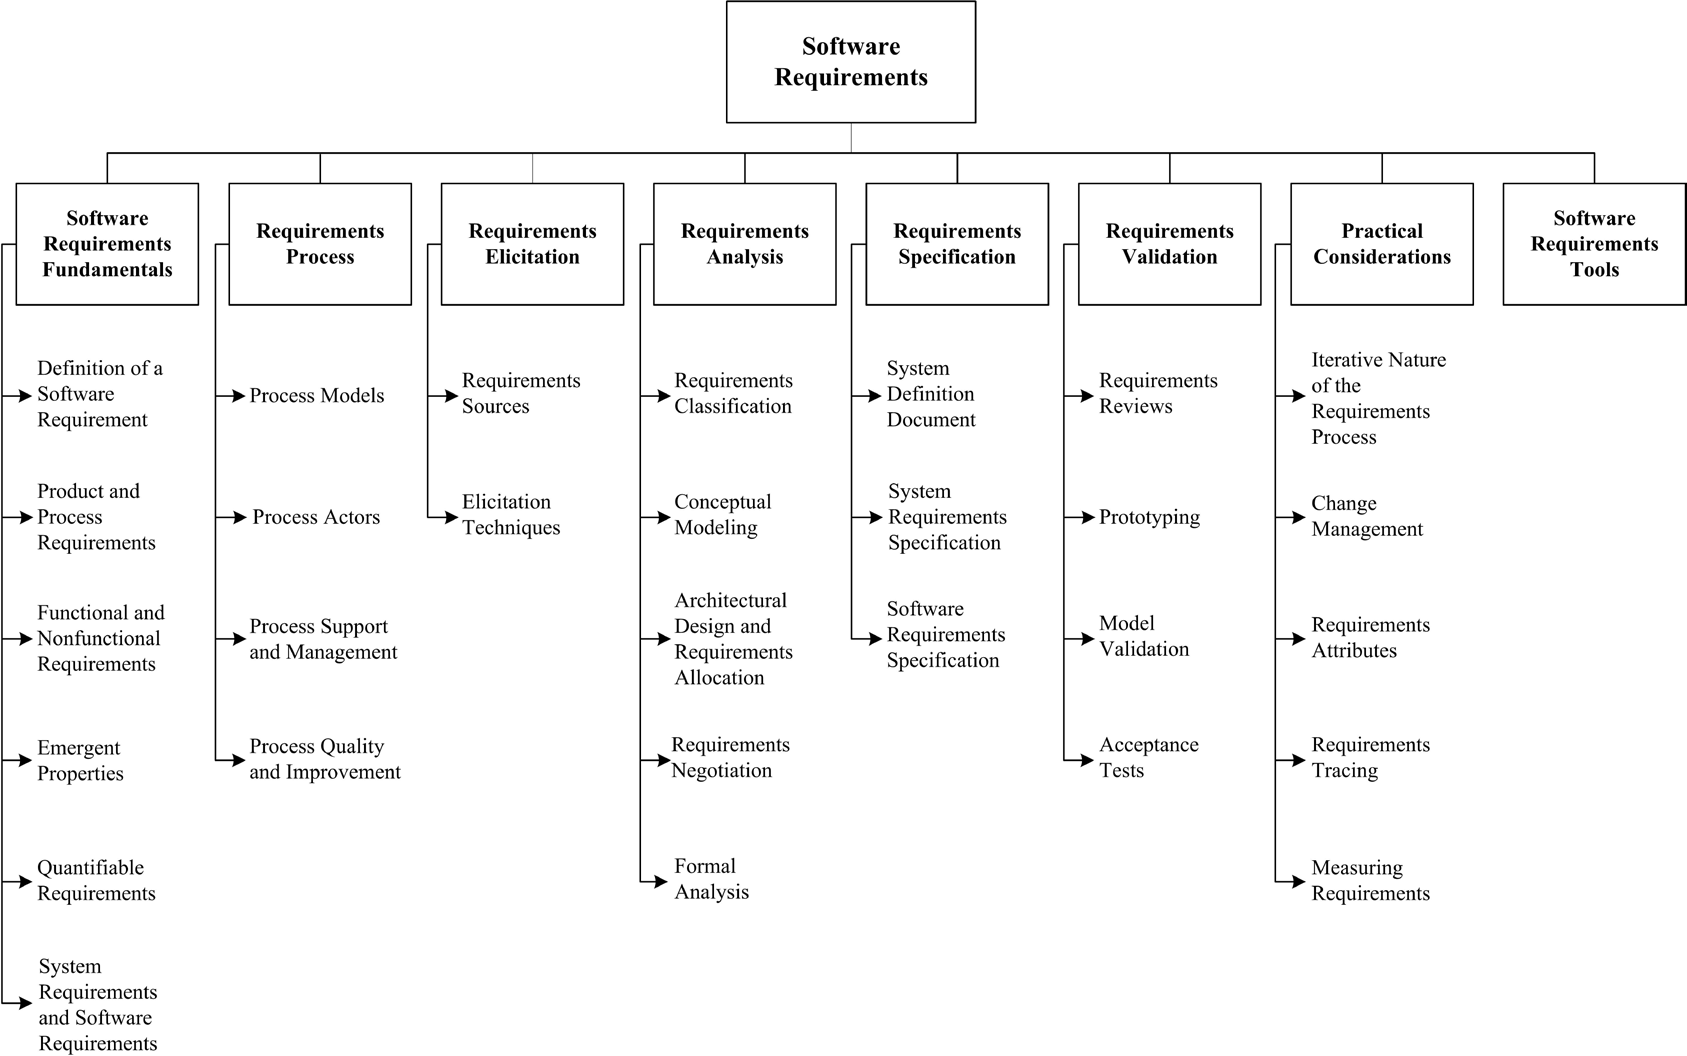
\includegraphics[width=\columnwidth]{swebooksoftwarerequirements}
\centering
\caption[Topics for software requirements]{Topics for the Software Requirements knowledge area~(\citetitle{SWEBOK}, \citeyear{SWEBOK})}
\label{fig:swebook_software_requirements}
\end{sidewaysfigure}

This section defines requirements engineering and breaks it down into its core processes and activities. We will not cover all topics contained in Figure~\ref{fig:swebook_software_requirements}, but instead focus on the more relevant ones, from the point of view of the work described in this thesis. 

The engineering aspect of requirements development and management, should not distract us from the fact that software development involves at least as much communication as it does computing, and yet we sometimes fail to appreciate that requirements engineering and, in particular, requirements elicitation -- and much of software and systems project work in general -- is primarily a human interaction challenge~\citep{Wiegers2013}. 

\subsection{Definition}
The definition in~\citefield{ieee_std_29148}{journaltitle} describes requirements engineering as an \emph{\textquote[][]{interdisciplinary function that mediates between the domains of the acquirer and supplier to establish and maintain the requirements to be met by the system, software or service of interest}}. A vital part of the systems engineering process, requirements engineering first defines the problem scope and then links all subsequent development information to it~\citep{Hull2011}. One of the most long-standing definition comes from a US Department of Defence software strategy document

\begin{displaycquote}{united1991department}
Requirements engineering involves all life-cycle activities devoted to identification of user requirements, analysis of the requirements to derive additional requirements, documentation of the requirements as a specification, and validation of the documented requirements against user needs, as well as processes that support these activities
\end{displaycquote}

A more recent definition emphasizes the goal-oriented nature of requirements engineering, and hints at the importance of understanding and documenting the relationships between requirements and other development artefacts

\begin{displaycquote}{Zave:1997:CRE:267580.267581}
Requirements engineering is the branch of software engineering concerned with the real world goals for, functions of, and constraints on software systems. It is also concerned with the relationship of these factors to precise specifications of software behaviour, and to their evolution over time and across software families
\end{displaycquote}

\citet{Hull2011} argues that both definitions omit the role that requirements play in accepting and verifying the solution. The authors propose an alternative definition

\begin{displaycquote}{Hull2011}
Requirements engineering is the subset of systems engineering concerned with the discovery, development, trace, analysis, qualification, communication and management of requirements that define the system at successive levels of abstraction
\end{displaycquote}

They argue the above definition is a better reflection that requirements exist at multiple levels of development, and also list key activities that are considered proper to requirements engineering. Similarly to what we have done for the definition of requirement, it is worth breaking this definition into its constituent parts. \emph{Discovery}, refers to activities related to the elicitation and capture of requirements; \emph{trace} allows setting up links to and from requirements to other artefacts; \emph{qualification} refers to all kinds of testing activities and avoids the often confusing terms \emph{validation} -- checking formal expressions of requirements against informal needs -- and \emph{verification}, often linked with checks of requirements internal consistency within and between layers of abstraction; \emph{communication} reflects the notion that requirements are part of a human activity, through which all stakeholders agree on what is to be achieved. Finally, the word \emph{abstraction} makes reference to the practice of organizing requirements into layers and of tracing the satisfaction relationship between those layers.

\citet{Hull2011} makes a useful extension to software requirements that applies to complete systems -- a collection of components, machine, software and human, which co-operate in an organised way to achieve some desired result. Since components must co-operate, interfaces between components are a vital consideration in system (and requirements) engineering, that is, interfaces between people and machine components, between machine components, and between software components.

\subsection{Processes}
Without loss of generality, we can say that requirements engineering can be split into two main processes, \emph{requirements development} and \emph{requirements management}. Requirements development can be subdivided into elicitation, analysis, specification, and validation~(\citetitle{SWEBOK},~\citeyear{SWEBOK}). Figure~\ref{fig:requirements_engineering_disciplines} below shows the domain of requirements engineering split into requirements development, encompassing the activities just mentioned, and also requirements management

\begin{figure}[h]
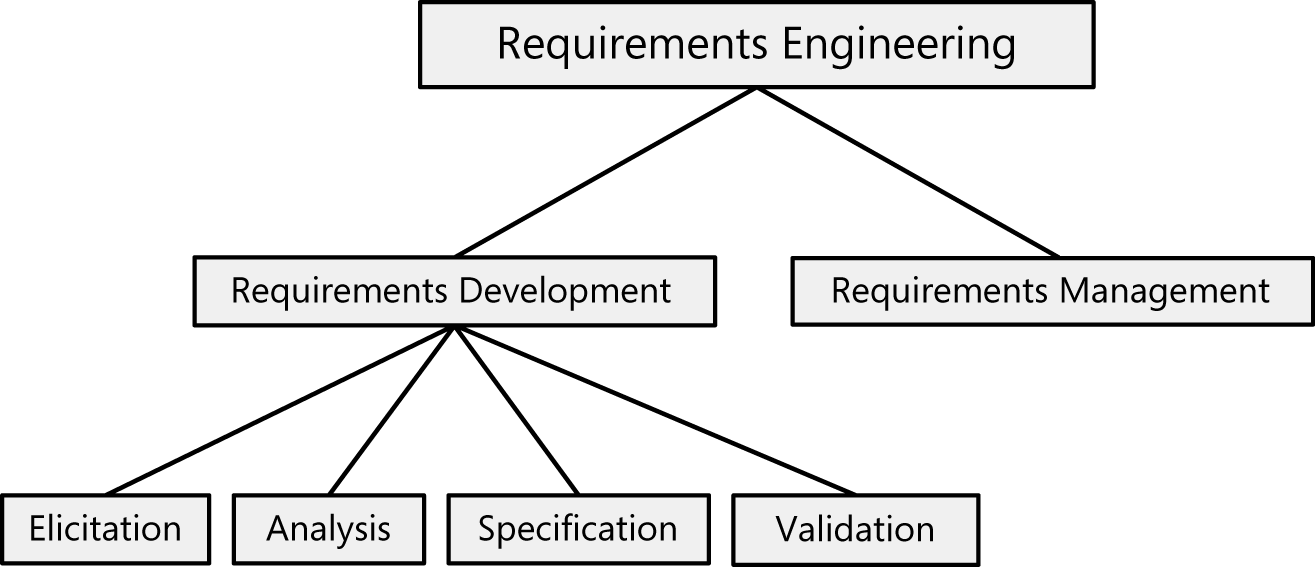
\includegraphics[width=0.75\textwidth]{RequirementsEngineeringDisciplines}
\centering
\caption[Requirements engineering disciplines]{Requirements engineering disciplines~\citep[p. 15]{Wiegers2013}}
\label{fig:requirements_engineering_disciplines}
\end{figure}

Regardless of the development life cycle followed -- be it pure waterfall, iterative, incremental, agile, or other -- these activities will be present, perhaps at different times in the project and to varying degrees of detail~\citep{Wiegers2013}. Following, are the essential actions in each sub-discipline

\emph{Requirements elicitation} encompasses all of the activities involved with discovering requirements, such as interviews, workshops, document analysis and others. It is a process through which, those who acquire and those who supply a given system, discover, review, articulate, understand, and document the requirements on the system and the life cycle processes~(\citefield{ieee_std_29148}{journaltitle}). It typically assumes either a usage-centric or a product-centric approach, although other strategies are also possible. The usage-centric strategy emphasizes understanding and exploring user goals to derive the necessary system functionality. The product-centric approach focuses on defining features that you expect will lead to marketplace or business success~\citep{Wiegers2013}.

The same standard defines \emph{requirements analysis} as a process that transforms stakeholder and requirement-driven views of desired services into technical views of products that could deliver those services. The main goal is to obtain a precise understanding of each requirement and representing sets of requirements in appropriate ways. This is done by distinguishing user's goals from functional requirements, determining quality expectations, business rules, suggested solutions, and other information~\citep{Wiegers2013}.

\emph{Requirements specification} involves representing and storing the collected knowledge and information in a persistent and well-organized fashion. The principal activity is translating the collected user needs into written requirements and, optionally visual models, suitable for comprehension, review and use by their intended audiences~\citep{Wiegers2013}.

\citefield{ieee_std_29148}{journaltitle} defines \emph{requirements validation} as a confirmation by examination that requirements (individually and as a set) define the right system as intended by the stakeholders. It confirms that information gathered will enable developers to build a solution that satisfies the business objectives. The central activities are reviewing the documented requirements to correct any problems before the development group accepts them; developing acceptance tests and criteria to confirm that a product based on the requirements would meet customer needs and achieve the business objectives~\citep{Wiegers2013}.

\citet{Wiegers2013} allude that, from a practical point of view, the goal of \emph{requirements development} is to accumulate a shared understanding of requirements that is good enough to allow construction of the next portion of the product, be that 1 or 100 percent of the entire product, to proceed at an acceptable level of risk. It is in line with what~\citefield{ieee_std_29148}{journaltitle} refers to as a \emph{baseline} set of requirements, that is, \emph{`a specification or product that has been formally reviewed and agreed upon, that thereafter serves as the basis for further development, and that can be changed only through formal change control procedures'}. The major risk is that, if not performed properly, having to do excessive unplanned rework because of insufficient understanding of the requirements for the next chunk of work before starting design and construction~\citep{Wiegers2013}.

\citefield{ieee_std_29148}{journaltitle} identifies processes and activities within, that are named differently, but that are in essence similar to the ones just described. The principal processes identified are \emph{stakeholder requirements definition} and \emph{requirements analysis} or \emph{system requirements analysis}. These two processes result in a baseline set of requirements, with a nature similar to the mentioned before. The architectural design process includes allocation and decomposition of requirements that triggers the recursive application of the requirements processes, for the definition of system element requirements and the iterative application of the requirements analysis process for derived requirements.

There is a common misconception that requirements engineering is just a single phase that is carried out and completed at the outset of product development~\citep{Hull2011}. On the contrary, requirements developed at the outset are still in use at the final stages of development. Figure~\ref{fig:testsandreqs} shows different testing activities and their relationship with requirements specified at various levels of abstraction. It is clear that stakeholder requirements are tested as part of acceptance test, a late stage in any software development method, be it traditional or agile. In addition, each testing activity has a separate concern, with acceptance test focusing on validating the product; system test verifying the system and integration and component testing, verifying subsystem and components requirements, respectively.
\begin{figure}[h]
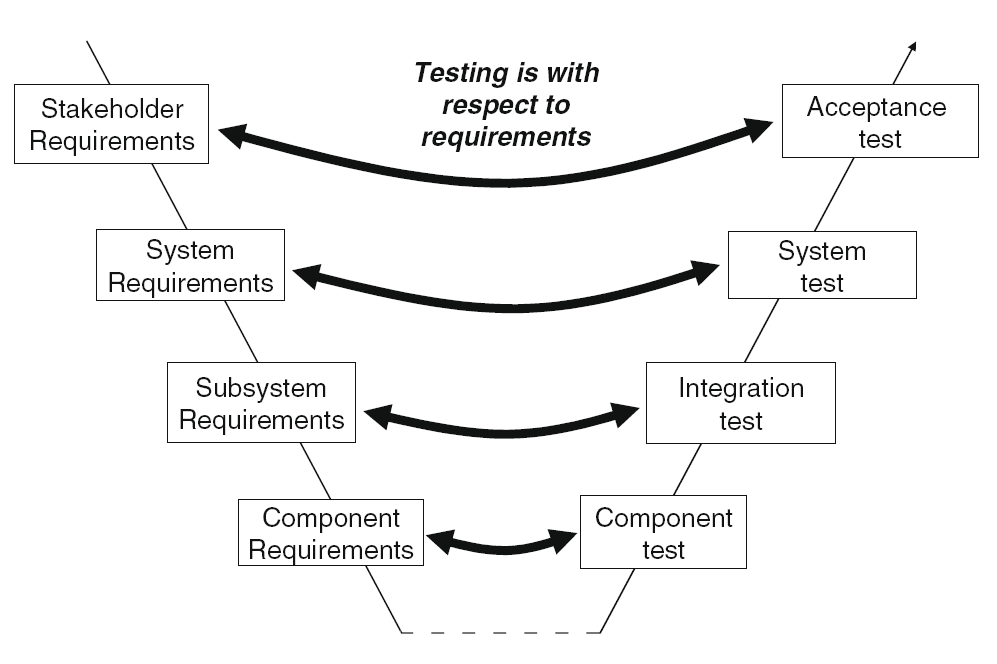
\includegraphics[width=0.75\textwidth]{RoleOfRequirementsInRelationToTesting}
\centering
\caption[Testing activities and requirements]{Testing activities and requirements~\citep{Hull2011}}
\label{fig:testsandreqs}
\end{figure}

If requirements are to play such a central role in systems development, they need to be maintained. Hence requirements engineering connects strongly with change management. Independently of where new or changed requirements come from, the impact of that change on quality, cost and schedule needs to be assessed. This assessment informs decisions to either accept or reject a change; negotiate the cost of change and organise and assign work to development teams~\citep{Hull2011}. The purpose of \emph{requirements management} is to anticipate and accommodate requirements changes, so as to minimize their disruptive impact on the project. Core requirements management activities include defining the requirements baseline; evaluating the impact of proposed requirements changes; establishing any relationships and dependencies between requirements and tracking requirements status and change activity throughout the project~\citep{Wiegers2013}.

The key concept that enables this kind of impact analysis is requirements tracing, primarily concerned with understanding how high-level requirements -- objectives, goals, aims, aspirations, expectations, needs -- are turned into low-level requirements. It is therefore primarily concerned with the relationships between layers of information. Requirements tracing allow measuring the impact of change, track progress against a set of requirements and assess benefit against cost of implementation~\citep{Hull2011}.

\section{Agile Requirements Engineering}
\label{sec:agile_requirements}
Traditional software development methods, such as waterfall~\footnote{~\citet{royce1970managing} is known to have first described the waterfall process, even though he did not use that term}, advocate a simple top-down flow of requirements information (see figure~\ref{fig:waterfall}). In this model, software development occurs in an orderly series of sequential stages. Requirements are agreed to, a design is created, and code follows thereafter. Lastly, the software is tested to verify its conformance to its requirements and design, and deployed to its users upon successful verification~\citep{Leffingwell2011}.

\begin{figure}[h!]
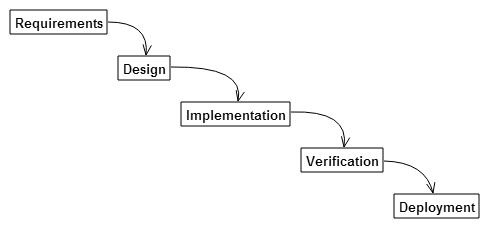
\includegraphics[width=0.60\textwidth]{waterfall2}
\centering
\caption[Sequential stages in waterfall development]{Sequential stages in waterfall development~\citep{Leffingwell2011}}
\label{fig:waterfall}
\end{figure}

The past decade has seen a movement to more lightweight and increasingly agile methods. Software technology has moved from supporting business operations to becoming a critical component of business strategy~\citep{Highsmith:2000:ASD:323922}. The move towards agile methods was driven by the same causes that led manufacturers to transition from mass production to lean production techniques, namely a focus on quality, cost reduction and an increase in speed to market.

We will not detail an historical perspective of the evolution from predictive, waterfall-like methods to iterative and incremental processes (e.g RUP~\footnote{~see \citetitle{Kruchten2003},~\citet{Kruchten2003} for details}) to the more recent agile and lean development methods~\citep{Leffingwell2011,Larman2003}. Instead, we describe an agile requirements artefact model and corresponding agile practices and principles, that compose the agile requirements approach found in current agile methods. In addition, we introduce BDD and explain it in the context of \emph{Specification by Example}~\citep{Adzic201106} practices and principles.

\subsection{Agile practices and principles}
The agile manifesto~\footnote{~see http://www.agilemanifesto.org/ for details} declares that: 
\emph{We are uncovering better ways of developing software by doing it and helping others do it. Through this work we have come to value}

\begin{itemize}
\item \textbf{Individuals and interactions} over processes and tools
\item \textbf{Working software} over comprehensive documentation
\item \textbf{Customer collaboration} over contract negotiation
\item \textbf{Responding to change} over following a plan
\end{itemize}
\emph{That is, while there are value in the items on the right, we value the items on the left more}

In each statement, the first part (in bold face) indicates a preference, whilst the other represents an item that, although relevant, is of lower priority. The authors of the manifesto chose their words carefully and the use of the word \emph{`uncovering'} and the expression \emph{`by doing it'}, place agile as a continuous incremental learning process carried out by practitioners in the software engineering field.

Agile development reverses the traditional approach of favouring processes and tools over people. In agile, the emphasis is much more on people collaboration and interaction than in following a plan or using a particular set of tools. Similarly, while comprehensive documentation is not a problem in itself, the emphasis should be in working software. Agile methods shift from strict contract negotiation to close collaboration between team members and customers, ensuring delivered software meets customer needs. Finally, agile realises that customer needs are not static and accepts changes to requirements, even if late in the project~\citep{Highsmith:2000:ASD:323922}. 

In agile development approaches we expect cycles and iteration among the business, user, and functional requirements~\citep{Wiegers2013} and where goals are defined for each iteration and are revisited once the iteration is completed~\citep{Inayat2015}. Often, it is impossible or unnecessary to fully specify functional requirements before commencing design and implementation. The essence of agile development is learning just enough about requirements to do thoughtful prioritization and release planning so teams can begin delivering valuable software as quickly as possible~\citep{Wiegers2013}.

In response to a somehow fragmented knowledge about the solutions that agile brought to requirements engineering and the new challenges it has raised,~\citet{Qasaimeh2008} reflect on the differences of `traditional' and agile requirements engineering, the practices adopted by the latter and the solutions and challenges presented by adoption of agile requirements. The study compared different agile development methods, analysed their characteristics and classified them based on key requirements for a software development project. The authors analysed some of the most popular agile software methods such as Scrum~\footnote{~see \citetitle{Schwaber:2001:ASD:559553},~ \citet{Schwaber:2001:ASD:559553} for details}, Extreme Programming~(XP)~\footnote{~see \citetitle{Beck:1999:EPE:318762},~ \citet{Beck:1999:EPE:318762} for details}, Feature Driven Development~(FDD)~\footnote{~see \citetitle{Palmer:2001:PGF:600044}~\citet{Palmer:2001:PGF:600044} for details}, Adaptive Software Development (ASD)~\footnote{~see \citetitle{Highsmith:2000:ASD:323922},~ \citet{Highsmith:2000:ASD:323922} for details} and Crystal Methodologies~\footnote{~see \citetitle{CockburnCrystal2004} and~ \citet{CockburnCrystal2004} for details}.

They concluded that \emph{customer involvement} is a key practice in all agile processes and all analysed methods consider customers an integral part of the development process. Some of the methods advocate the presence of the customer on-site to elicit, prioritize and verify requirements and also during acceptance testing, where most agile processes require tests to be written and executed by customers.

To reduce \emph{time to market}, most agile processes favour early delivery of software so that customers can use the software and provide feedback early on, improving defect rates and the customers understanding of the expected software features. Agile processes have the ability to quickly \emph{respond to change}, with some processes relying on daily meetings with users, and promoting direct user interaction in determining changes to requirements and deciding what and when changes to requirements are going to be implemented. An informal approach to \emph{documentation} is favoured and agile processes advocate face to face communication and presence of on-site user representatives.

The practices described are not specific to an agile development method, but rather have evolved from multiple uses and empirical studies of commonality across methods. A recent systematic literature review paper~\citep{Inayat2015915} identified the most common agile practices of agile requirements engineering (see Table~\ref{tb:agile_practices}).
\ifdraft{%
  \fxnote{THIS WILL CONTAIN TABLE OF AGILE PRACTICES}
}{%
\begin{table}[h!]
\caption[Agile practices]{List of popular agile practices~\citep{Inayat2015915}}
\label{tb:agile_practices}
\setlength{\extrarowheight}{1.8pt}
\centering
\scalebox{0.75}{
\begin{tabularx}{\textwidth}{cX}
\toprule \multicolumn{1}{c}{\bfseries{Practice}}&
\multicolumn{1}{c}{\bfseries{Description}}\\
\addlinespace
\midrule
Acceptance tests & In an agile context, refer to tests created and applied for each of the defined user stories, confirming their correctness and determining the completeness of a user story implementation. In practice, acceptance tests are small notes written at the back of story cards\\ \midrule
Code refactoring & 
To restructure software by applying a series of changes to the internal structure of software to make it easier to understand and cheaper to modify without changing its observable behaviour\\ \midrule
Cross-functional teams & A group of individuals with different functional expertise working towards a common goal. In agile methods, developers, testers, designers, and managers work closely together, helping to bridge communication gaps~\citep{Adzic:2009:BCG:1538647}\\ \midrule
Customer involvement & Agile methods rely on frequent collaboration with an accessible and available on-site customer\\ \midrule
Face-to-face communication & Agile processes advocate minimal documentation in the form of user stories and discourage long and complex specification documents, favouring frequent face-to-face communication\\ \midrule
Iterative requirements & Unlike in traditional software development methods, requirements emerge over time in agile methods through frequent interaction among stakeholders and gradual detailing of requirements\\ \midrule
Prototyping &  Promotes quicker feedback and enhances customer anticipation of the product, allowing timely feedback prior to moving to subsequent iterations\\ \midrule
Requirements management &  Performed by maintaining
product backlog/feature lists and index cards\\ \midrule
Requirements prioritisation & In agile methods, requirements are prioritised continuously in each development cycle by customers who focus on business value\\ \midrule
Retrospectives & At regular intervals, the team reflects on how to become more effective, then tunes and adjusts its behaviour accordingly~\footnotemark\\ \midrule
Testing before coding & Commonly known as Test Driven Development, means to write tests prior to writing functional codes for requirements. It promotes feedback in the case of test failures\\ \midrule
User Stories & Are created as specifications of the customer requirements. User stories facilitate communication and better overall understanding among stakeholders. A user story describes functionality of a system or software and is composed of a written description used for planning and as a reminder; follow-up conversations that serve to flesh out the details of the story and tests that convey and document details and that can be used to determine when a story is complete~\citep{cohn2004user}.\\
\addlinespace
\bottomrule
\end{tabularx}
}
\end{table}
\footnotetext{~see http://www.agilemanifesto.org/ for details}
}
All agile processes place focus on \emph{verification and validation} of requirements, using testing techniques such as unit, integration and regression testing. Other quality review techniques are also used such as design and code inspections, retrospectives and code quality reviews. They also foster team communication and collaborative work by doing daily `stand ups' -- started in Scrum and now widely accepted as common practice, where all team members stand up around a circle, hence the name `stand ups', for about 10 to 15 minutes and discuss what they have been doing since the last time they met and any issues or blockers they may be faced with -- and use of code standards for facilitating exchange of information among team members.

\subsection{Agile requirements artefact model}
Nowadays, a significant number of organizations have made the transition to agile and that has brought to light common patterns for agile software processes. ~\citet{Leffingwell2011} introduces the idea of the \emph{Agile Enterprise Big Picture} (see figure~\ref{fig:scaled_agile_framework}) with the goal of sharing a language for discussion, a set of abstractions, and a visual model that describes agile software development and delivery process mechanisms, the teams and organizational units, and some of the roles key individuals play in the new agile paradigm. The vocabulary introduced is a method-independent set of constructs widely used in the industry and generally accepted in current agile development practices.

\begin{figure}[h]
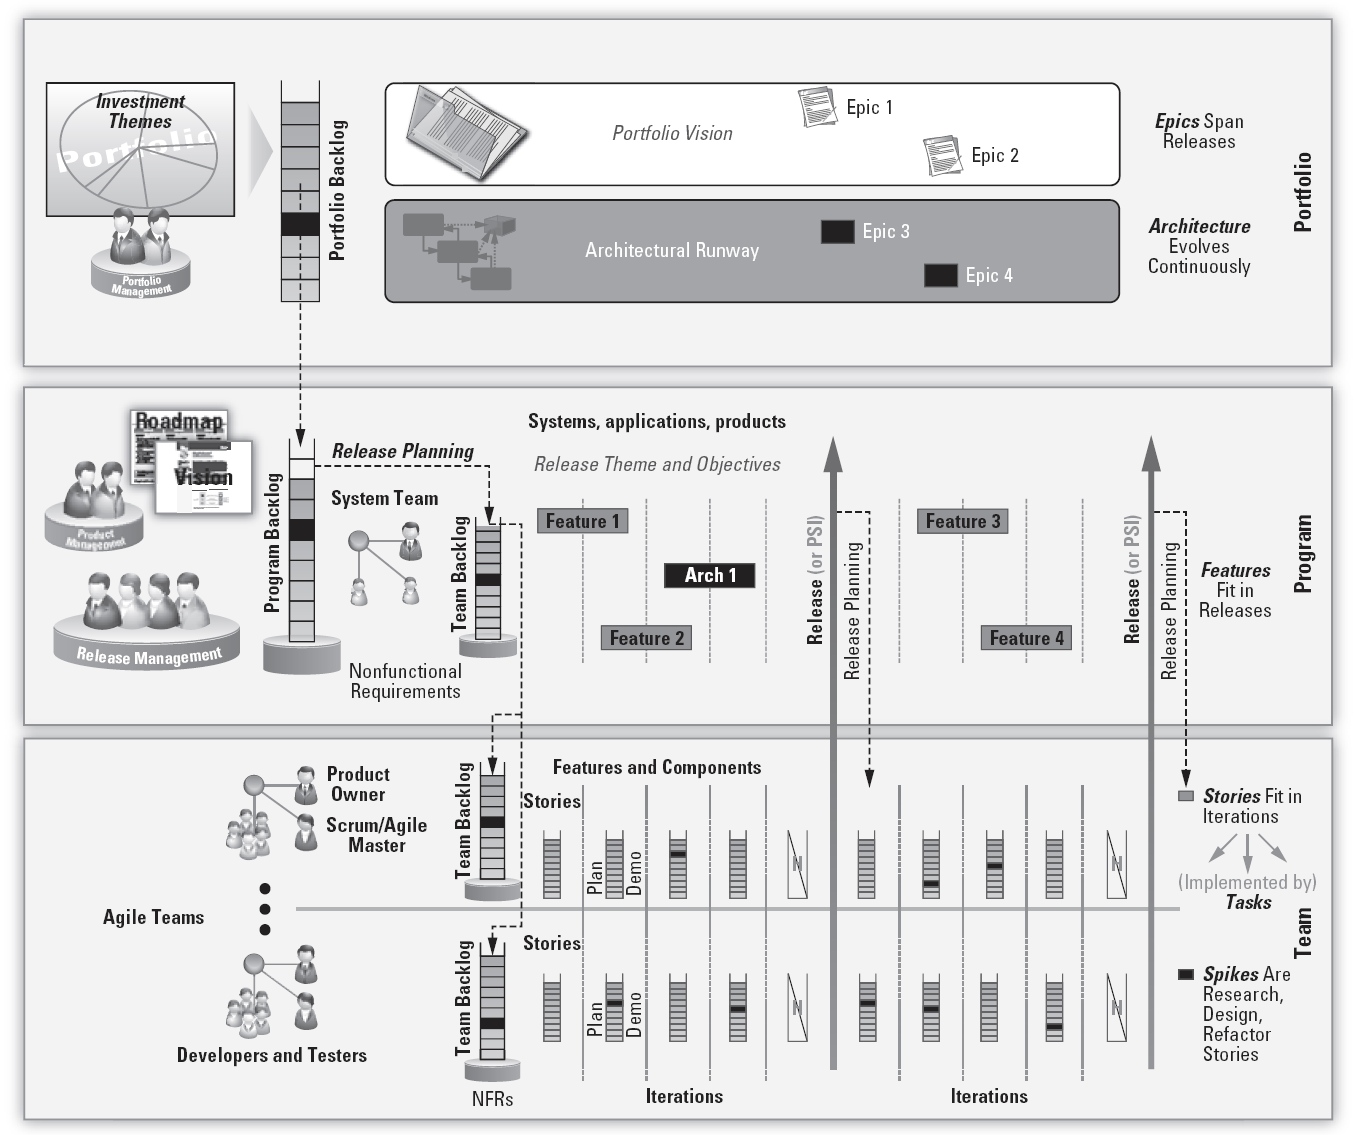
\includegraphics[width=0.95\textwidth]{ScaledAgileFrameworkbw}
\centering
\caption[Agile enterprise]{Agile development levels: \emph{Team}, \emph{Program} and \emph{Portfolio}~\citep{Leffingwell2011}}
\label{fig:scaled_agile_framework}
\end{figure}

\citeauthor{Leffingwell2011} describes agile at scale at different levels of detail and with increasing abstraction, from \emph{Team} to \emph{Program} and finally \emph{Portfolio}. 

At the \emph{Team} level
\begin{displaycquote}{Leffingwell2011}
... agile teams define, build, and test user stories in a series of iterations and releases. In the smallest enterprise, there may be only a few such teams. In larger enterprises, groups, or pods, of agile teams work together to support building up larger functionality into complete products, features, architectural components, subsystems, and so on. The responsibility for managing the backlog of user stories belongs to the team's product owner
\end{displaycquote}

At the \emph{Program} level
\begin{displaycquote}{Leffingwell2011}
...the development of larger-scale systems functionality is accomplished via multiple teams in a synchronized standard cadence of time-boxed iterations and milestones that are date and quality fixed, but scope is variable, producing releases or potentially shippable increments (PSI) at frequent, typically fixed, 60 to 120 day time boundaries.
\end{displaycquote}

At the \emph{Portfolio} level
\begin{displaycquote}{Leffingwell2011}
... a mix of themes are used to drive the investment priorities for the enterprise. That construct assures that the work being performed is the work necessary for the enterprise to deliver on its chosen business strategy. Investment themes drive the portfolio vision, which is expressed as a series of larger, epic-scale initiatives, which will be allocated to various release trains over time
\end{displaycquote}

In the context of this thesis, \emph{Team} and \emph{Program} levels are the most relevant. In addition, together with an agile requirements artefact meta-model (see figure~\ref{fig:metamodel_partial}), we are in possession of an unambiguous and coherent language for doing research in agile requirements engineering. We will delve less into the organisational and team composition aspects of the model, but instead focus on the elements introduced by the meta-model.

\begin{figure}[h]
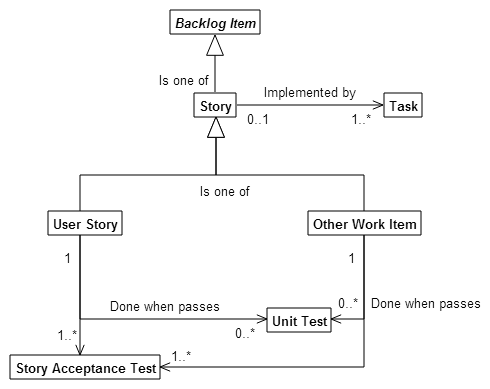
\includegraphics[width=0.65\textwidth]{metamodel_partial2}
\centering
\caption{Agile requirements meta-model for the \emph{Team}}
\label{fig:metamodel_partial}
\end{figure}

The meta-model defines the concept of a \emph{Backlog Item} -- an abstract entity representing something that needs to be done, either a user story or another work item -- and a \emph{Backlog}, a repository of all the work items the team has identified. This backlog is the one and only definitive source of work for the team. A \emph{Story} is the rough equivalent of a software requirement in agile and, at the \emph{Team} level, we distinguish two types: a \emph{User Story} -- used to define the system behaviour and determine value for the user -- and \emph{other work items} such as defects, documentation, support and maintenance activities, infra-structure work and so on. \citet{Leffingwell2011} defines \emph{Story} as \emph{`a work item contained in the team's backlog'} and \emph{User Story} as \emph{`a brief statement of intent that describes something the system needs to do for the user'}.

\emph{Tasks} are used to breakdown a \emph{Story} in work activities required to its implementation. Note that \emph{Tasks} can exist on their own and without an associated \emph{Story}, if the work activity is considered independent and can standalone. Also, a \emph{Story} requires one or more tasks for its implementation and is only complete when it passes one or more \emph{acceptance tests}. A \emph{Story} could also be subject to \emph{unit tests} to confirm that the lowest-level module of an application or module of an application works as intended.

\begin{figure}[!h]
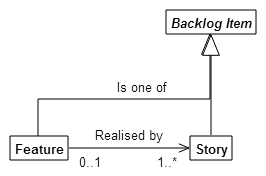
\includegraphics[width=0.50\textwidth]{metamodel_features2}
\centering
\caption{Agile requirements meta-model (\emph{Features})}
\label{fig:metamodel_features}
\end{figure}

At \emph{Program} level, the backlog contains a prioritized set of \emph{features} intended to deliver benefits to the users. \citet{Leffingwell2011} defines \emph{Features} as \emph{`services provided by the system that fulfil stakeholder needs'}. \emph{Features} are a kind of backlog item as can be seen in figure~\ref{fig:metamodel_features}. \emph{Features} are at a higher level of abstraction than \emph{Stories} and sit between needs of users and software requirements, expressed in agile as \emph{Stories}. A given \emph{Feature} is realised by one or more \emph{Stories}.

\begin{figure}[h]
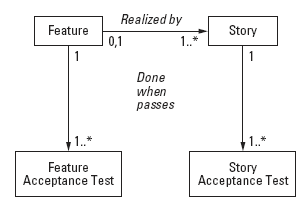
\includegraphics[width=0.50\textwidth]{metamodel_features_tests}
\centering
\caption{Agile requirements meta-model (\emph{Features} and \emph{Acceptance Tests})}
\label{fig:metamodel_features_tests}
\end{figure}

Similar to \emph{Stories}, \emph{Features} also require acceptance tests to ensure all stories that realise it are complete. Note that a \emph{Feature acceptance test} is not a composition of \emph{Story acceptance tests}, as they should focus on other types of tests such as performance, `what-if' scenarios, etc. 

\emph{Features} and \emph{Stories} are used to specify the functionality of a system but we should not ignore non-functional requirements. In the model in figure~\ref{fig:metamodel_nfrs}, we see first that some backlog items may be constrained by non-functional requirements, and some may not. We also see that non-functional requirements may not apply to backlog items, meaning that they stand independently and apply to the system as a whole~\citep{Leffingwell2011}.

\begin{figure}[h]
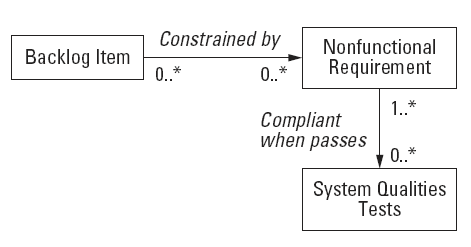
\includegraphics[width=0.55\textwidth]{metamodel_nfrs}
\centering
\caption{Agile requirements meta-model (\emph{Non-functional requirements})}
\label{fig:metamodel_nfrs}
\end{figure}

It is important to note that a non-functional requirement constrains a \emph{Backlog item} which can be either \emph{Features} or \emph{Stories}. This is important from a practical perspective as it is not uncommon to have agile teams starting with \emph{Features} to organise their \emph{backlog}. This is also the case in some agile approaches such as the one described in the next section.

\subsection{Behaviour driven development~(BDD)}
\label{ch:Background:sec:bdd}
\citet{Hull2011} advocates the use of modelling techniques as a mechanism of fostering understanding and communication of ideas associated with system development. A good model is one which is easily communicated. They need to be used for communication within a development team, and also to an organisation as a whole including the stakeholders. The uses of a model can be diverse and cover a wide spectrum. It might be to model the activities of an entire organisation or to model a specific functional requirement of a system. It is this latter use that receives the attention of Behaviour Driven Development which is, in its essence, an approach to derive the functionality of a system or component from business goals using concrete examples~(see figure~\ref{fig:bdd_from_goals_to_specs}).

In the foreword to \citetitle{Smart201410}, Dan North the creator of BDD states the following \emph{`... (BDD) was a response to a triple conundrum: programmers didn't want to write tests; testers didn't want programmers writing tests; and business stakeholders didn't see any value in anything that wasn't production code'}.

BDD applies at all levels of software development, from high-level requirements discovery and specification to detailed low-level coding, whilst promoting the discovery of requirements and automation of high-level acceptance criteria, build and verification of the design and implementation, and production of accurate and up-to-date technical and functional documentation.~\citep{Smart201410}.

\begin{figure}[h]
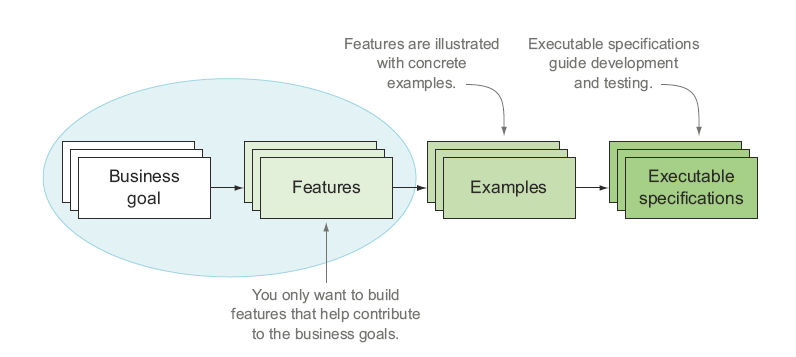
\includegraphics[width=0.75\textwidth]{BDD}
\centering
\caption[From business goals to executable specifications]{BDD: From business goals to executable specifications~\citep{Smart201410}}
\label{fig:bdd_from_goals_to_specs}
\end{figure}

BDD helps teams focus their efforts on identifying, understanding, and building valuable features that matter to businesses, and it makes sure that these features are well designed and well implemented~\citep{Smart201410}. BDD practitioners use conversations around concrete examples of system behaviour to help understand how features will provide value to the business. Furthermore, it encourages business analysts, software developers, and testers to collaborate more closely by enabling them to express requirements in a more testable way, in a form that both the development team and business stakeholders can easily understand. Tools exist that can help turn these requirements into automated tests that help guide the developer, verify the feature, and document what the application does~\citep{Smart201410,wynne2012cucumber}. Figure~\ref{fig:bdd_from_goals_to_specs} depicts the typical flow of information in BDD, from business goals to features, followed by identification of concrete examples, all part of a specification that gets tested and verified against initial business goals stated.

\begin{figure}[h]
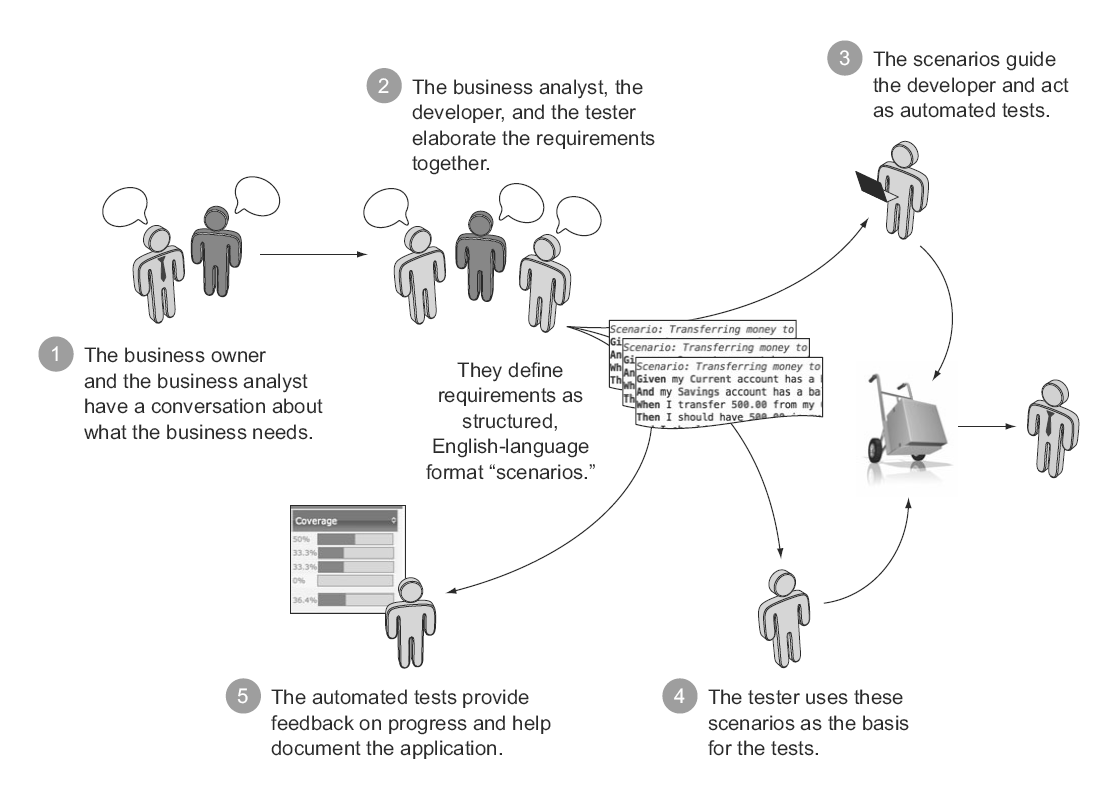
\includegraphics[width=0.95\textwidth]{communication_in_bdd}
\centering
\caption[Improved communication in BDD]{Improved communication in BDD~\citep{Smart201410}}
\label{fig:communication_in_bdd}
\end{figure}

Some authors and practitioners do not consider BDD a software development methodology in its own right, but as a set of methods and techniques grouped under the same label, which incorporates, builds on, and enhances ideas from many agile and iterative methodologies~\citep{Smart201410}.

It is important to note that BDD was developed as a mechanism for fostering collaboration, improving communication and requirements discovery through examples. In traditional development methods, requirements follow a sequential set of activities where typically a business owner informs an analyst of his needs and goals, who in turn will write a requirements document that a developer translates into software. Simultaneously, or upon development is complete, a tester translates the same requirements document into test cases which, if executed with success, lead to user and technical documentation being produced and the software being deployed to end-users. In BDD the focus is on collaboration, with all interested parties sharing a structured specification that is used to simultaneously, specify features to be implemented and tests to be executed.

BDD can also be seen as an instance of \emph{Specification by Example}~\citep{Adzic201106} as they both share a common set of principles and practices. \emph{Specification by example} introduces a consistent and coherent language for patterns, ideas and artefacts used for teams who derive \emph{executable specifications} and \emph{living documentation} from \emph{business goals}. The practices of \emph{Specification by Example} do not form a fully fledged software development methodology but rather supplement other methodologies -- both iterative and flow based -- to provide rigour in specifications and testing, enhance communication between various stakeholders and members of the software development team~\citep{Adzic201106}.

\begin{figure}[h]
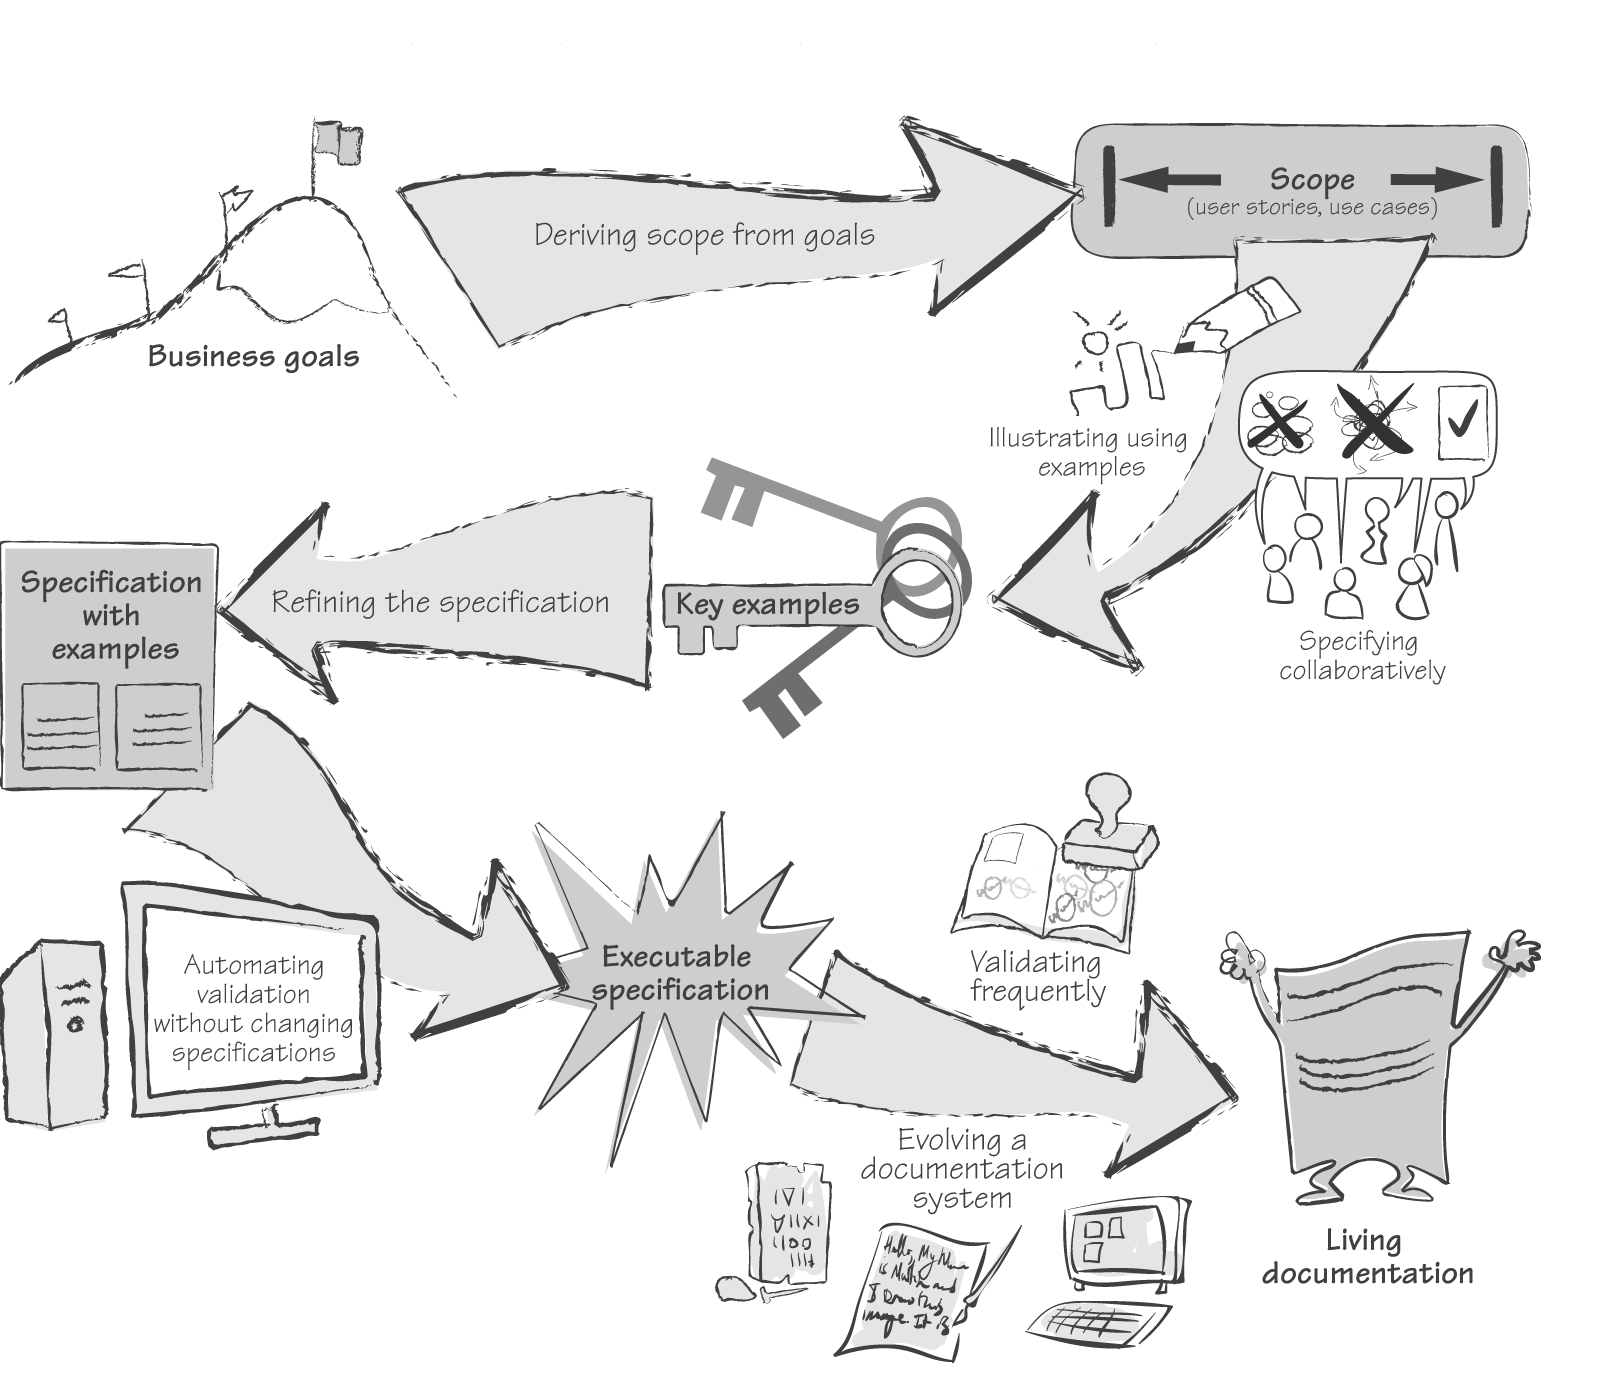
\includegraphics[width=0.9\textwidth]{SpecificationbyExample}
\centering
\caption[Specification by Example]{Process patterns of \emph{Specification by Example}~\citep{Adzic201106}}
\label{fig:specification_by_example}
\end{figure}

Instead of relying on users to provide requirements, teams \emph{derive scope from goals}, taking customer's business goals and defining the scope in terms of the set of features that achieve those goals. This is done collaboratively with business users and team members, to improve communication and reduce unnecessary rework. \emph{Specifying collaboratively} they are able to harness the knowledge and experience of all team members. It also creates a collective ownership of specifications, making everyone more engaged in the delivery process~\citep{Adzic201106}.

Teams \emph{illustrate specifications using examples}. The team works with business users to identify key examples describing expected functionality, flushing out functional gaps and inconsistencies and ensuring that everyone involved has a shared understanding of what needs to be delivered, avoiding rework that results from misinterpretation and translation~\citep{Adzic201106}.

\emph{Key examples} must be concise to be useful. By \emph{refining the specification}, successful teams remove extraneous information and create a concrete and precise context for development and testing. They define the target with the right amount of detail to implement and verify it. They identify what the software is supposed to do, not how it does it~\citep{Adzic201106}.

Once a team agrees on \emph{specifications with examples} and refines them, the team can use them as a target for implementation and a means to validate the product. To get the most out of key examples, successful teams automate validation without changing the information. As they\emph{ automate validation without changing specifications}, the key examples are always comprehensible and accessible to all team members. An automated \emph{Specification with examples} that is comprehensible and accessible to all team members becomes an \emph{executable specification}. We can use it as a target for development and easily check if the system does what was agreed on, and we can use that same document to get clarification from business users~\citep{Adzic201106}.

\emph{Validating frequently} executable specifications against the system ensures we can discover any differences between the system and the specifications and keep both synchronised in face of changes to requirements or implementation. Not only do teams validate frequently, they also ensure that specifications are actual, current and consistent, effectively turning them into \emph{living documentation}.

In BDD, \emph{executable specifications} are expressed using \emph{Gherkin}~\citep{wynne2012cucumber}, a domain specific language used to specify desired features of a system or application (see feature~\ref{lst:feature_example} for an example of a specification in Gherkin). 

\begin{featurelist}{Example of a feature file in Gherkin~\citep{wynne2012cucumber}}{lst:feature_example}
\begin{featurecode}{0.7}
\begin{minted}{Gherkin}
Feature: Feedback when entering invalid credit card details

  In user testing we've seen a lot of people who made mistakes
  entering their credit card. We need to be as helpful as possible
  here to avoid losing users at this crucial stage of the
  transaction.

  Background:
    Given I have chosen some items to buy
    And I am about to enter my credit card details

  Scenario: Credit card number too short
    When I enter a card number that's only 15 digits long
    And all the other details are correct
    And I submit the form
    Then the form should be redisplayed
    And I should see a message advising me of the correct number of digits

  Scenario: Expiry date invalid
    When I enter a card expiry date that's in the past
    And all the other details are correct
    And I submit the form
    Then the form should be redisplayed
    And I should see a message telling me the expiry date must be wrong
\end{minted}
\end{featurecode}
\end{featurelist}

\emph{Gherkin} specifications are  defined from plain-language text files called \emph{feature files}, containing scenarios to implement and test, representing concrete examples of the features being specified. Each scenario is a list of steps for a BDD tool such as Cucumber to work through~\citep{wynne2012cucumber}. These tools parse feature files turning each scenario step into source code, typically a method call in one of the tool's supported languages. 
Feature~\ref{lst:feature_example} displays a feature file, specified in \emph{Gherkin}, for a credit card application containing two scenarios with concrete examples of credit card validation rules. In Gherkin, we use the \emph{Feature} keyword to name (text after \emph{Feature} keyword, excluding colon character) and describe (all remaining text until the next keyword) a feature. Gherkin uses the \emph{Background} keyword to specify a set of steps that are common to every scenario and within each scenario \emph{Given} is used to set up the context where the scenario happens, \emph{When} to interact with the system somehow and \emph{Then} to check that the outcome of that interaction was what we expected. \emph{And} and \emph{But} keywords are used to make specifications more readable and take the same role as the keyword in the previous line.

\subsection{Summary}

In this chapter we have provided definitions of requirements and presented them within the context of requirements engineering. We followed with an analysis of core activities of requirements engineering and described how they manifest in the context of agile development methods. Finally, we introduced BDD in context with \emph{Specification by Example} and gave an example a feature specification in Gherkin.

It is important to state that in BDD, and other agile approaches in general, handling of non-functional requirements is ill defined. Customers or users talking about what they want the system to do normally do not think about resources, maintainability, portability or performance~\citep{Paetsch:2003tl}. In the next chapter we will explore further the notion of non-functional requirements, present some well known classification schemes, and methods used for their elicitation and analysis with a focus on goal-oriented approaches and GRL~\citep{Amyot2010}, in particular.

\chapter{On non-functional requirements}
\label{ch:nfr_research}
\iftoggle{chapterthree}
{
    \fxnote{Chapter 3 will go here}
}
{
In the previous chapter we have followed a generic approach to requirements engineering, without focusing on any particular requirement type. In this chapter, we take a different view and focus on the concept of \nfrs in requirements engineering.

It is consensual that a system's utility is determined by both its functional and non-functional characteristics, such as usability, flexibility and performance~\citep{Chung:2009vg}.

The perception of quality is determined by these two characteristic sets, and therefore, they must be taken into consideration in the development of software systems. However, most of the attention in software engineering in the past has been centred on notations and techniques for defining and providing the functions of a software system~\citep{Chung:2009vg}. Additionally, in the occasions where non-functional characteristics are taken into consideration, they are treated only as technical issues related mostly to the detailed design or testing of an implemented system~\citep{Chung:2009vg}.

\citet{Chung:2009vg} noted that real-world problems are more non-functionally oriented than they are functionally oriented, e.g., poor productivity, slow processing, high cost, low quality and unhappy customers. Rather than worry about precisely how to refer to these information types, it is more pertinent to ensure they are part of requirements elicitation and analysis activities. A product can be delivered with the desired functionality but that users hate because it doesn't match their (often unstated) quality expectations~\citep{Wiegers2013}.

In the remainder of this chapter, we will highlight issues with current definitions of non-functional requirements. We will also list relevant classification and representation schemes. Finally, we will introduce goal-oriented approaches to handling non-functional requirements, with a focus on goal-oriented requirements language (GRL).

\section{Definition}
For many years, the requirements for a software product have been classified broadly as either functional or non-functional. The functional requirements are evident: they describe the observable behaviour of the system under various conditions. However, many people dislike the term `non-functional'~\citep{Wiegers2013}. 

These `other-than-functional' requirements, could refer to \emph{how} well a system performs its functions, rather than to \emph{what} those functions may be. They could describe important characteristics or properties of a system, such as availability or performance. Likewise, they could be considered as \emph{quality attributes}~(\citefield{ieee_std_1061}{journaltitle}), but that view ignores other aspects such as design and implementation constraints or business rules, which we could also view as non-functional characteristics~\citep{Wiegers2013}.

We now provide three selected definitions, not because of their special correctness or attractiveness, but because they are amongst the more popular ones and support the argument that present definitions are inconsistent, ambiguous and confusing at times~\citep{Glinz:2007ehba}.

\citet{Wiegers2013} defines non-functional requirements as
\begin{displaycquote}{Wiegers2013}
... descriptions of a \emph{property} or \emph{characteristic} that a software system must exhibit or a \emph{constraint} that it must respect, other than an observable system behaviour
\end{displaycquote}

while \citet{Jacobson:1999:USD:309683} defines them as
\begin{displaycquote}{Jacobson:1999:USD:309683}
.. a requirement that specifies system properties, such as environmental and \emph{implementation constraints}, performance, platform dependencies, maintainability, extensibility, and reliability. A requirement that specifies \emph{physical constraints} on a functional requirement.
\end{displaycquote}

and \citet{Sommerville:1998:REP:552009} as requirements which are
\begin{displaycquote}{Sommerville:1998:REP:552009}
... not specifically concerned with the functionality of a system, instead specifying restrictions on the product being developed and the development process, and \emph{external constraints} the product must meet.
\end{displaycquote}

\citet{Glinz:2007ehba} identifies terminological, but also major conceptual issues with current definitions of non-functional requirements. Most definitions use the terms \emph{property} or \emph{characteristic}, \emph{attribute}, \emph{quality} or \emph{constraint} differently, and the meaning of those terms is not always clear. For example, \emph{property} and \emph{characteristic} denote something that the system must have, but that is equally a criteria for inclusion in functional requirements definitions. Also, every non-functional requirement (or functional, for this matter) can be regarded as a quality of a system or as a constraint, because it restricts the space of potential solutions to those that meet this requirement~\citep{Glinz:2007ehba}. In addition, there are references to implementation, physical and external constraints and not only there is a lack of clear guidance as to what they intend to restrict, also, these restrictions or constraints are known by different terms in other definitions, such as \emph{`interface requirements'} or \emph{`design constraints'}. Finally, \emph{performance} is treated as a quality or attribute is most definitions, but it deserves a category of its own in some quality models~(\citefield{ieee_std_29148}{journaltitle}).

\section{Classification and representation schemes}

The definitions we have just alluded to, refer to concepts that are considered to be part of non-functional requirements. However, there are more detailed classification schemes that are worth our attention.

\citet{Roman:1985} provides one such classification scheme based on the notion of constraints and types of constraints. \emph{Interface} constraints, define the way components of a system or application and its environment, interact. \emph{Performance} constraints, cover a broad range of issues dealing with time/space bounds, reliability, security, and survivability. \emph{Operating} constraints, include physical (e.g., size, weight, power, etc.), personnel availability, skill level considerations, accessibility for maintenance, environmental conditions (e.g., temperature, radiation, etc.), and spatial distribution of components. \emph{Life-cycle} constraints, fall into two broad categories: those that pertain to qualities of the design, such as maintainability or portability, and those that limit the development, maintenance, and enhancement process. \emph{Economic} constraints, represent considerations relating to immediate and long term costs. Finally, \emph{political} constraints deal with policy and legal issues. This view of non-functional requirements as constraints of components of a system or application will be explored further in Chapter~\ref{ch:Extendingbdd}.

Another classification scheme is introduced by~\citefield{ieee_std_9126One}{journaltitle} and its interpretation of software quality. Software product quality can be evaluated by measuring internal attributes (typically static measures of intermediate products), or by measuring external attributes (typically by measuring the behaviour of the code when executed), or by measuring quality in use attributes. The objective is for the product to have the required effect in a particular context of use.

This standard defined a quality model for external and internal quality. It categorises software quality attributes into six characteristics (functionality, reliability, usability, efficiency, maintainability and portability), which are further subdivided into sub-characteristics

\begin{figure}[h]
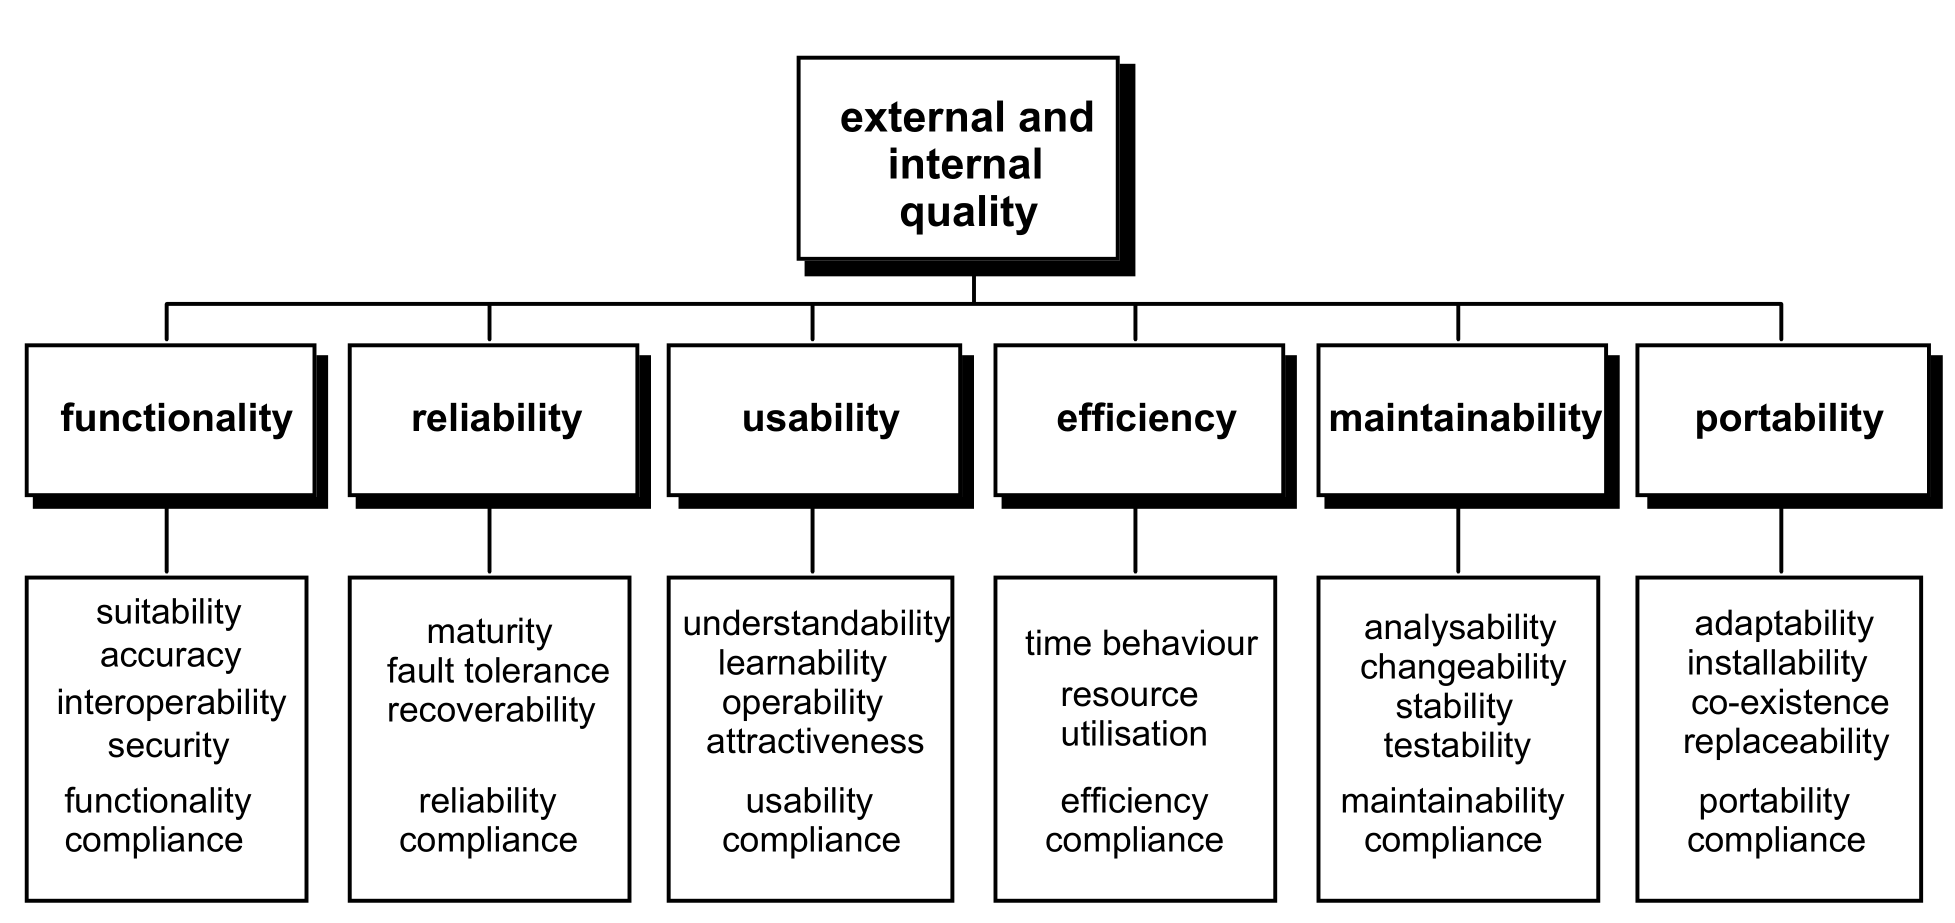
\includegraphics[width=0.95\textwidth]{QualityInLifecycle}
\centering
\caption[Software product quality model]{Software product quality model in ~\citefield{ieee_std_9126One}{journaltitle}}
\label{fig:QualityInLifecycle}
\end{figure}

Interestingly, several issues have been identified with~\citefield{ieee_std_9126One}{journaltitle} such as terminology inconsistencies with other ISO standards; ambiguities in the way it is structured in terms of characteristics and sub-characteristics; incomplete set of characteristics and sub-characteristics, etc.~\citep{Al-Qutaish}.

\begin{figure}[h]
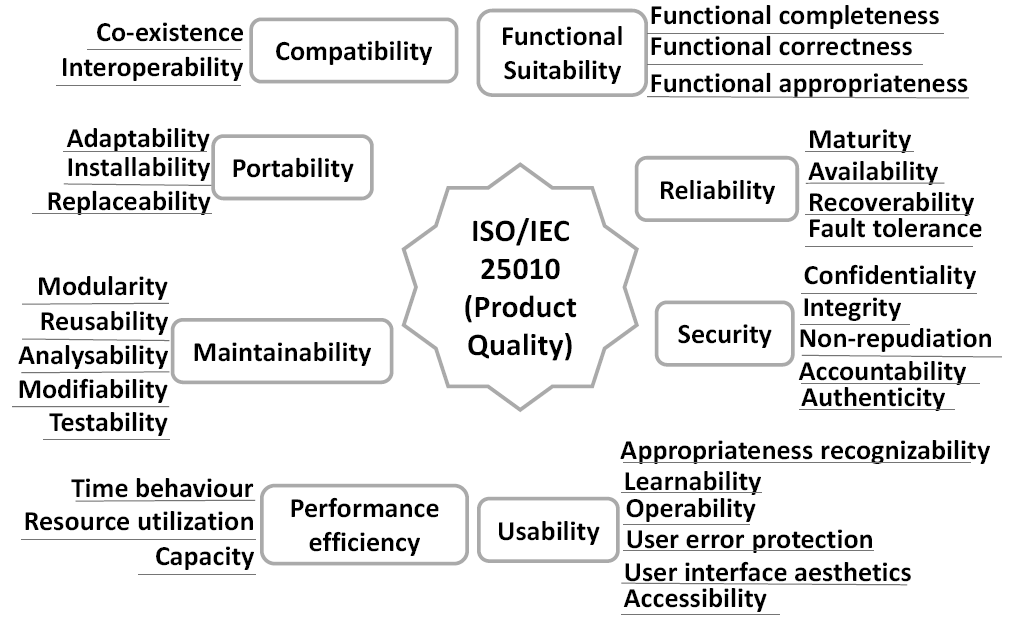
\includegraphics[width=0.65\textwidth]{iso25010}
\centering
\caption[ISO 25010 quality model]{ISO 25010 quality model in ~\citefield{ieee_std_25010}{journaltitle}}
\label{fig:iso25010}
\end{figure}

This has lead to a revised standard that extends this quality model with eight product quality characteristics and 31 sub-characteristics~(\citefield{ieee_std_25010}{journaltitle}) (see figure~\ref{fig:iso25010}).

Another classification sheme is FURPS~\citep{Grady1987}, an acronym representing a model for classifying software quality attributes or non-functional requirements, based on five categories: functionality, usability, reliability, performance and supportability~(see table~\ref{tb:furps}). The original FURPS model was later extended to empathize various specific attributes~\citep{adams2015non}.
\ifdraft{%
  \fxnote{THIS WILL CONTAIN FURPS TABLE}
}{%
\begin{table}[h!]
\caption[FURPS quality model]{FURPS quality model~\citep{Grady1987}}
\label{tb:furps}
\setlength{\extrarowheight}{1.8pt}
\centering
\scalebox{0.75}{
\begin{tabularx}{0.55\textwidth}{cX}
\toprule \multicolumn{1}{c}{\bfseries{Category}}&
\multicolumn{1}{l}{\bfseries{Attribute}}\\
\addlinespace
\midrule
\multirow{4}{*}{Functionality} & Feature set \\
& Capabilities \\ 
& Generality \\ 
& Security \\ \midrule
\multirow{4}{*}{Usability} & Human factors \\
& Aesthetics \\ 
& Consistency \\ 
& Documentation \\ \midrule
\multirow{5}{*}{Reliability} & Frequency/severity of failure \\
& Recoverability \\ 
& Predictability \\ 
& Accuracy \\
& Mean time to failure \\ \midrule
\multirow{5}{*}{Performance} & Speed \\
& Efficiency \\ 
& Resource consumption \\ 
& Throughput \\
& Response time \\ \midrule
\multirow{9}{*}{Supportability} & Testability \\
& Extensibility \\ 
& Adaptability \\ 
& Maintainability \\
& Compatibility \\
& Configurability \\
& Serviceability \\
& Installability \\
& Localizability \\
\addlinespace
\bottomrule
\end{tabularx}
}
\end{table}
}

Some classification schemes emerge from research work carried out in specific domains. For example, in the context of Service Oriented Architectures (SOA)~\footnote{~https://en.wikipedia.org/wiki/Service-oriented\_architecture}, ~\citet{Hanane2012} defined a catalogue of generic (i.e., domain independent) non-functional properties to be considered when service descriptions are developed including reliability, usability and security, but also others less obvious such as price -- the fee that the service consumer is expected to pay for invoking a given service -- or reputation of service, understood as the opinion of service consumers towards a service.

A more recent classification scheme is provided by~\citet{adams2015non}. In this work, over 200 non-functional requirements are reduced, using results reported in eight models from the extant literature. The 27 resultant non-functional requirements have been organized in a taxonomy that categorizes the 27 major nonfunctional requirements within four distinct categories: \emph{System Design Concerns}, \emph{System Adaptation Concerns}, \emph{System Viability Concerns} and \emph{System Sustainment Concerns}. Figure~\ref{fig:nfrs_in_systems_design} show the relationship between the four system concerns and the 27 non-functional requirements selected for consideration during a system's life cycle.

\begin{figure}[h]
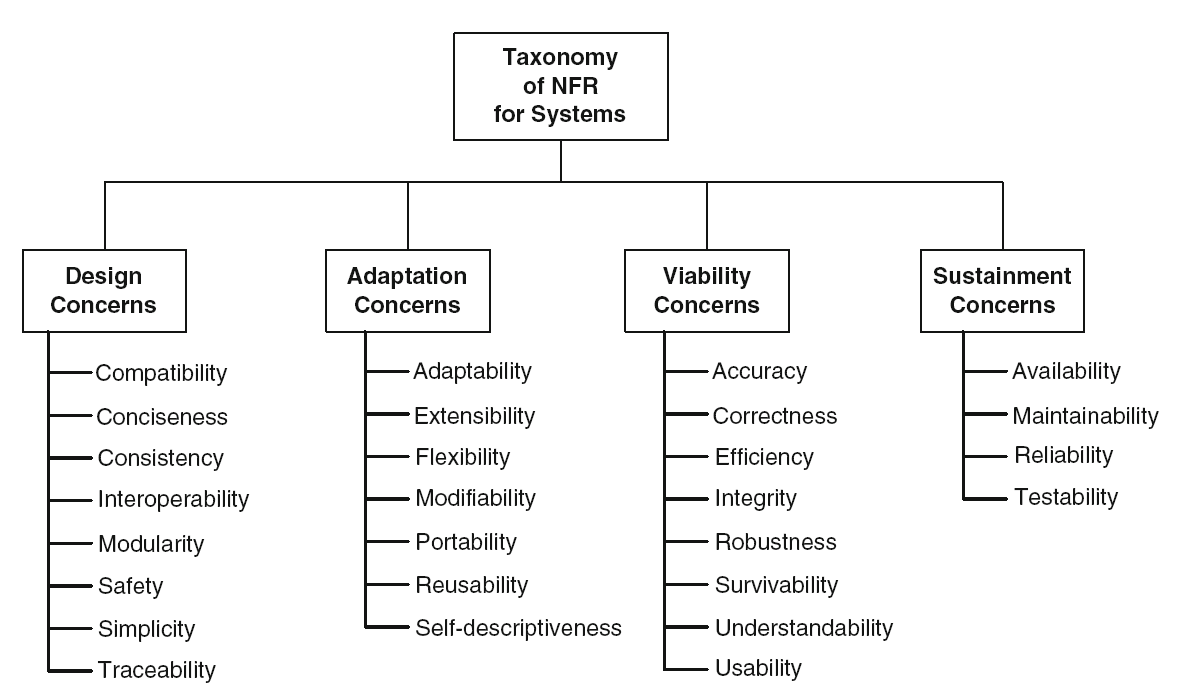
\includegraphics[width=0.95\textwidth]{nfrs_in_systems_design}
\centering
\caption[Taxonomy of non-functional requirements for systems]{Taxonomy of non-functional requirements for systems~\citep{adams2015non}}
\label{fig:nfrs_in_systems_design}
\end{figure}

There have also been attempts to automate the classification of non-functional requirements. One of such approaches, detects and classifies stakeholders quality concerns across requirements specifications containing scattered and non-categorized requirements, and also across free-form documents such as meeting minutes or notes~\citep{Cleland-Huang:2007}. A similar approach, proposes a semi-supervised text categorization for the automatic identification and classification of non-functional requirements~\citep{Casamayor:2010}.

According to \citet{Glinz:2007ehba}, the categorization and sub-classification of non-functional requirements in current classification schemes, reflect rather divergent concepts. For instance, whilst~\citet{Roman:1985} presents a classification scheme based on the notion of constraints, \citet{adams2015non} devises another scheme around concerns. Glinz had previously found more classification problems due to mixing three concepts that should better be separated. These are the concepts of \emph{kind} (should a given requirement be regarded as a function, a quality, a constraint, etc.), \emph{representation} and \emph{satisfaction} (hard vs. soft requirements)~\citep{Glinz:2005unba}.

A software practitioner should be aware of the well known classification schemes and their limitations, such as the terminology and categorically inconsistencies mentioned above. More than be concerned with choosing the right scheme, he or she should know what each attribute or quality characteristic means, such as performance, so that the correct intent can be communicated between users, developers and testers who, ultimately, will implement and verify appropriate features in the product or application~\citep{Chung:2009vg}.

According to~\citet{Matoussi:2008wr}, there are three extreme ways of specifying software requirements: complete formal specifications, informal specifications and hybrid or semi-formal approaches. We proceed by sampling from the literature, several approaches belonging to the above mentioned categories.

\emph{No-Fun}~\citep{Franch1998} belongs to the formal category of representation schemes. \emph{NoFun} (acronym for `NOn-FUNctional'), is a formal language for the description of software quality consisting of a hierarchy of software quality characteristics and attributes formulated as abstract and concrete quality models; component quality descriptions through assignment of values to component quality basic attributes, and finally, quality requirements stated over components, both context-free (universal quality properties) and context-dependent (quality properties for a given framework software domain, company, project, etc.)~\citep{Franch1998}. In another paper~\cite{NoFunWithISO}, the framework was applied to the set of quality attributes refinements that are part of~\citet{ieee_std_9126One}.

\citet{Chung:2009vg} mention that an informal and common way to represent non-functional requirements is by means of requirements sentences, which are commonly listed separately under different sections of a requirements document and refers to~\citefield{ieee_830}{journaltitle}, superseded by~\citefield{ieee_std_29148}{journaltitle}, as an example.

There are also informal but structured approaches around requirements sentences, such as the \emph{Volere} requirements process~\citep{Robertson:1999}, that is comprised of an identification number, NFR type, use case related to it, description, rationale, originator, fit criterion, customer satisfaction, customer dissatisfaction, priority, conflicts, supporting material, and history~\citep{Chung:2009vg}.

In spite of all of the above ways by which non-functional requirements have been classified and represented, goal-oriented approaches were the first to treat \nfrs in more depth, dealing with their representation but also conflict detection amongst multiple non-functional requirements. 

\section{Goal-oriented approaches}
The use of goals in requirements engineering has received increasing attention over the past few years. Such recognition has led to a whole stream of research on goal modelling, goal specification, and goal-based reasoning for multiple purposes, such as requirements elaboration, verification or conflict management, and under multiple forms, from informal to qualitative to formal~\citep{Lamsweerde:2001wpba}.

A goal captures, at different levels of abstraction, the various objectives the system under consideration should achieve~\citep{Lamsweerde:2001wpba}. Goals also cover functional concerns associated with the services to be provided, and non-functional ones, associated with quality of service, such as safety, security, accuracy, performance, and so forth.

The \emph{NFR Framework}~\citep{Chung2000} has probably been the first requirements model to address the lack of a proper treatment of quality characteristics by addressing both functional and non-functional requirements as a whole, and at a higher level of abstraction for both the problem and the solution~\citep{Chung:2009vg}.

In the \emph{NFR Framework}, non-functional requirements are treated as softgoals, i.e., goals that need to be addressed not absolutely but in a good enough sense. Reflecting the sense of `good enough', the \emph{NFR Framework} introduces the notion of satisficing, and, with this notion, a softgoal is said to satisfice (instead of satisfy) another softgoal. Softgoals are related through relationships which represent the influence or interdependency of one softgoal on another. A qualitative analysis method is included in the framework for deciding the status of softgoals, given that other, related softgoals are satisfied or have been found to be unsatisfiable~\citep{Chung2000}.

\begin{figure}[h]
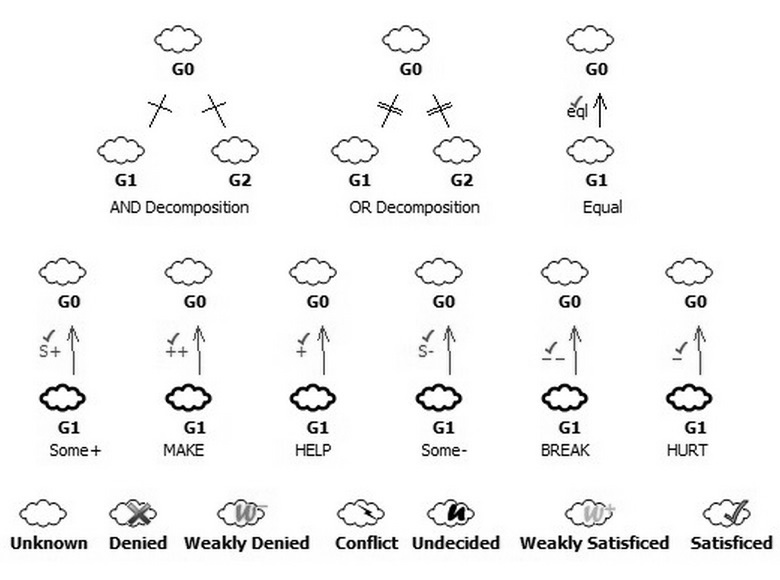
\includegraphics[width=0.75\textwidth]{SIGLegend}
\centering
\caption[Catalogue of visual elements in NFR Framework]{Catalogue of visual elements in NFR Framework~\footnotemark}
\label{fig:sig_legend}
\end{figure}
\footnotetext{~sourced from  http://www.utdallas.edu/~supakkul/NFR-modeling/label-evaluation}

Figure~\ref{fig:sig_legend} shows in graphical form the most important concepts of the \emph{NFR Framework}. Softgoals, which are `soft' in nature, are shown as clouds and can be decomposed in other more specific soft-goals though decomposition links. We say that softgoals are refined downwards into subgoals, and subgoals contribute upwards to parent softgoals. There are two main types of decompositions \emph{AND} and \emph{OR}, with the former used when several subgoals are needed together to meet a higher softgoal, and the latter when one subgoal alone is sufficient. 

When the non-functional requirements have been sufficiently refined, the next step is to identify \emph{operationalisations} (tick dark clouds), which are possible development techniques or specific solutions for achieving these non-functional requirements. In the \emph{NFR Framework}, each softgoal or contribution is associated with a \emph{label}, indicating the degree to which it is satisficed or denied.

The \emph{NFR Framework} offers several different types of contributions whereby a softgoal satisfices, or denies, another softgoal - \emph{MAKE}, \emph{HELP}, \emph{HURT} and \emph{BREAK} are the prominent ones. While \emph{MAKE} and \emph{BREAK} respectively reflect our level of confidence in one softgoal fully satisficing or denying another, \emph{HELP} and \emph{HURT} respectively reflect our level of confidence in one softgoal partially satisficing or denying another~\citep{Chung:2009vg}. 

The NFR Framework uses non-functional requirements such as security, accuracy, performance and cost to drive the overall design process. The framework, offers a structure for representing and recording the design and reasoning process in graphs, called softgoal interdependency graph (SIG)~\citep{Chung2000}. 

Main requirements are shown as \emph{softgoals} at the top of a graph. Softgoals are connected by \emph{interdependency links}, which are shown as lines, often with arrowheads. Softgoals have associated \emph{labels} (values representing the degree to which a softgoal is achieved) which are used to support the reasoning process during design~\citep{Chung2000}. 

Figure~\ref{fig:account_nfrs} shows a SIG for a hypothetical credit card application where security of account information, and good performance in the storing and updating of that information have been elicited as non-functional requirements to attain.

\begin{figure}[h]
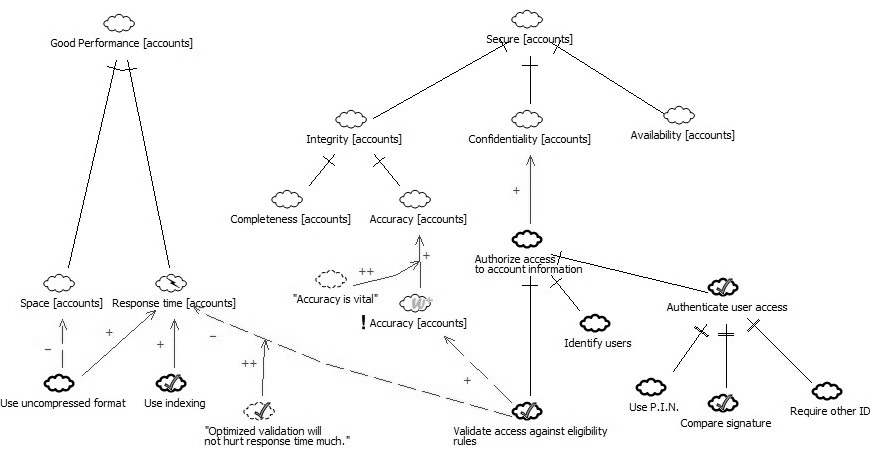
\includegraphics[width=0.95\textwidth]{AccountNFRs2}
\centering
\caption[Example of a Softgoal Interdependency Graph]{Example of a Softgoal Interdependency Graph (SIG)~\footnotemark}
\label{fig:account_nfrs}
\end{figure}
\footnotetext{~sourced from  http://www.utdallas.edu/~supakkul/NFRs-catalog/}

These two non-functional requirements, softgoals in the \emph{NFR Framework} terminology, are represented as clouds at the top of the figure. Softgoals have a type (in this case, security and performance) and a topic, which refers to an entity from the domain or subject matter, in this case bank accounts. In the figure, secure accounts softgoal is decomposed into sub-softgoals integrity, confidentiality and availability. In this case, the developer or designer has taken the view that authorizing access to account information would help attain confidentiality of accounts softgoal. This authorization access, is then refined into an \emph{OR} decomposition of operationalisations, namely `Use pin', `Compare signature' or `Require other ID'.

Faced with those options, a decision is made to compare signatures by labelling the `compare signature' operationalisation as satisficed, which in turn will do the same to `Authenticate user access'.

The \emph{NFR Framework}, rationalizes the development process by providing techniques for justifying design decisions made. These design decisions may positively or negatively affect one or more non-functional requirements, establishing interdependencies that allow inferring the degree to which those non-functional requirements are satisficed or denied~\citep{Chung2000}.

Handling non-functional requirements is complex, as it is difficult to define a non-functional term completely unambiguously and hard to explore a complete list of possible solutions and choose the best, or optimal solution~\citep{Chung:2009vg}. Therefore, the \emph{NFR Framework} takes a more lightweight and qualitative approach towards non-functional requirements, taking a view that softgoals are idealizations and, as such, without all its defining properties necessarily established.

\citet{Horkoff2012} suggests that models focusing on stakeholder goals are particularly suitable for elicitation and analysis in early requirements engineering, as they can show the underlying motivations for systems, capture non-functional success criteria, and show the effects of high-level design alternatives on the attainment of goals. We call this type of model, including agents with interdependent goals, agent-goal models, of which \emph{i*} and GRL are some of the most prominent examples.

The \emph{i*} framework incorporates concepts from the \emph{NFR framework}, including softgoals, \emph{AND/OR} decompositions, and contribution links, as well as (hard) goals, resources, and dependencies between actors (agents)~\citep{Horkoff2013}. \emph{i*} consists of two main modelling components. The \emph{Strategic Dependency (SD)} model is used to describe the dependency relationships among various actors in an organizational context. The \emph{Strategic Rationale (SR)} model is used to describe stakeholder interests and concerns, and how they might be addressed by various configurations of systems and environments~\citep{Yu1997}.

\begin{figure}[h]
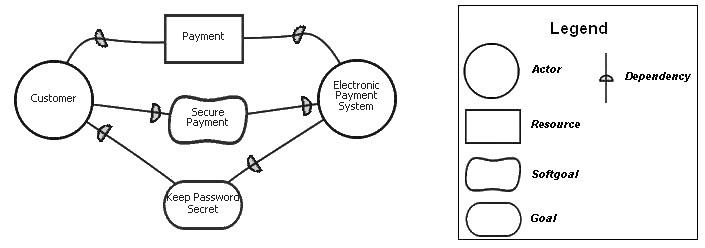
\includegraphics[width=0.95\textwidth]{istar_example}
\centering
\caption[Example of an \emph{i*} Strategic Dependency (SD) model]{Example of an \emph{i*} Strategic Dependency (SD) model~\citep{Roy:2007wyba}}
\label{fig:istar_example}
\end{figure}

Figure~\ref{fig:istar_example} shows a simple SD model with two actors represented by circles, a Customer and an Electronic Payment System, and their inter-dependencies. In the example, Payment represents a resource to be provided by the Customer, Secure Payment is a softgoal to be achieved by the System, and Keep Password Secret is a goal to be achieved by the Customer~\citep{Roy:2007wyba}.

The central concept in \emph{i*} is that of the intentional actor. Organizational actors are viewed as having intentional properties such as goals, beliefs, abilities, and commitments. Actors depend on each other for goals to be achieved, tasks to be performed, and resources to be furnished. By depending on others, an actor may be able to achieve goals that are difficult or imp 	ossible to achieve on its own~\citep{Yu1997}.

The concepts of \emph{actors} and \emph{intentional elements} in \emph{i*} have influenced other goal-oriented languages, and in particular GRL, a visual modelling notation for intentions, business goals, and non-functional requirements of many stakeholders, for alternatives that have to be considered, for decisions that were made, and for rationales that helped make these decisions~\citep{amyot2011user}. We describe GRL in depth in the next section.

\subsection{Goal-oriented Requirements Language~(GRL)}
\label{sec:gore}
The Goal-oriented Requirements Language (GRL)~\citep{Amyot2010}, inherits the concept of softgoal from the \emph{NFR Framework}, and adopts non-functional characteristics and related attributes, as first class modelling concepts~\citep{Chung:2009vg}. GRL captures business or system goals, alternative means of achieving goals (either objectively or subjectively), and rational for contributions and decisions~\citep{Amyot2003}. The language was developed with the following capability targets~\citep{Amyot2003}

\begin{itemize}
\item to enable reasoning about feature interactions and trade-offs early in the design process
\item to support the specification, analysis and management of goals and non-functional requirements
\item to model the relationship between goals and system requirements
\item to capture reusable analysis and design knowledge about non-functional requirements
\end{itemize}

GRL is part of User Requirements Notation (URN)~(\citefield{ituZ151}{journaltitle}), an ITU-T approved standard, with two complementary notations: GRL for modelling actors and their intentions, goals and non-functional requirements and Use Case Maps (UCM) notation for describing scenarios and architectures~\citep{Amyot2003}.~\citefield{ituZ151}{journaltitle} focuses on the definition of an abstract syntax, a concrete graphical syntax, and an interchange format for URN. In this section we will only cover what pertains to GRL as UCM is out of scope. 

GRL is a visual modelling notation for intentions, business goals, and non-functional requirements of stakeholders, for alternatives that have to be considered, decisions that were made, and rational that helped make these decisions~\citep{amyot2011user}.

There are four main categories of concepts in GRL: \emph{actors}, \emph{intentional elements}, \emph{indicators} and \emph{links}. Figure~\ref{fig:grl_visualsyntax} shows a summary of the graphical notation in GRL

\begin{figure}[h]
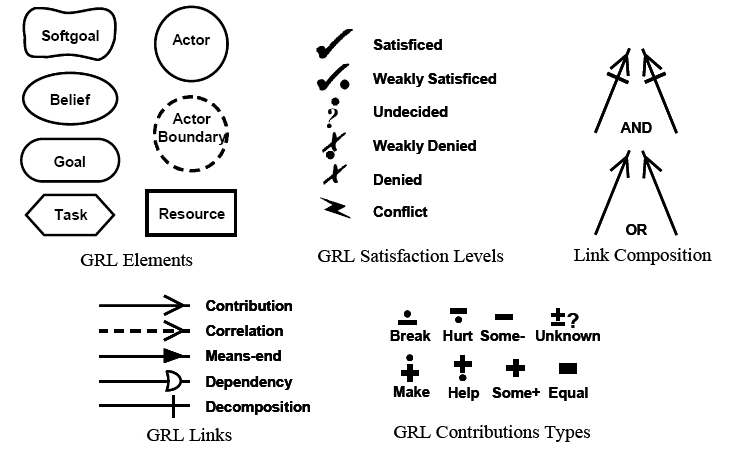
\includegraphics[width=0.75\textwidth]{grl_visualsyntax}
\centering
\caption[Summary of the GRL graphical notation]{Summary of the GRL graphical notation~\citep{Roy:2007wyba}}
\label{fig:grl_visualsyntax}
\end{figure}

The intentional elements in GRL are \emph{goals}, \emph{softgoals}, \emph{tasks}, \emph{resources} and \emph{beliefs}. \emph{Intentional} elements are used to present the different alternative behavioural (dynamic) and structural (static) aspects of the system requirements and concentrate on the rational for choosing a particular alternative over the others~\citep{Saleh2004}.

\emph{Actors} are holders of intentions; they are the active entities in the system or its environment (e.g., stakeholders or other systems) who want goals to be achieved, tasks to be performed, resources to be available and softgoals to be satisfied~(\citefield{ituZ151}{journaltitle}). \emph{Indicators} make real-world measurements available for reasoning in the goal model, allowing for a more accurate assessment of the satisfaction of actors~(\citefield{ituZ151}{journaltitle}). 

\emph{Softgoals} differentiate themselves from \emph{goals} in that there is no clear, objective measure of satisfaction for a softgoal whereas a goal is quantifiable, often in a binary way. Softgoals are often more related to non-functional requirements, whereas goals are more related to functional requirements~\citep{amyot2011user}.

\emph{Links} are used to connect isolated elements in the requirement model. Different types of links depict different structural and intentional relationships (including \emph{decompositions}, \emph{contributions} and \emph{dependencies})~(\citefield{ituZ151}{journaltitle}).

GRL supports the analysis of strategies, which help reach the most appropriate trade-offs among (often conflicting) goals of stakeholders. A \emph{strategy} consists of a set of intentional elements and indicators that are given initial satisfaction values~(\citefield{ituZ151}{journaltitle}). It uses qualitative labels associate to lower-level intentional elements to measure the satisfaction level of higher-level elements. The qualitative satisfaction labels associated to intentional elements goes from \emph{SATISFICED} to \emph{DENIED}~\citep{Roy:2007wyba}. These satisfaction values are then propagated to the other intentional elements through their links, enabling a global assessment of the strategy being studied as well as the global satisfaction of the actors involved~(\citefield{ituZ151}{journaltitle}).

The GRL notation supports belief elements, which provide justifications of the assessments in the model. Beliefs keep track of the rationales in the graphical models~\citep{Roy:2007wyba}.

The URN standard describes the syntax and semantics of the language using an abstract syntax (partially shown in figure~\ref{fig:grl_abstract_grammar}), reserving a concrete grammar, presented as an extension of the abstract grammar, to support a graphical language but which has no implication in the semantics of the language.

\begin{figure}[h]
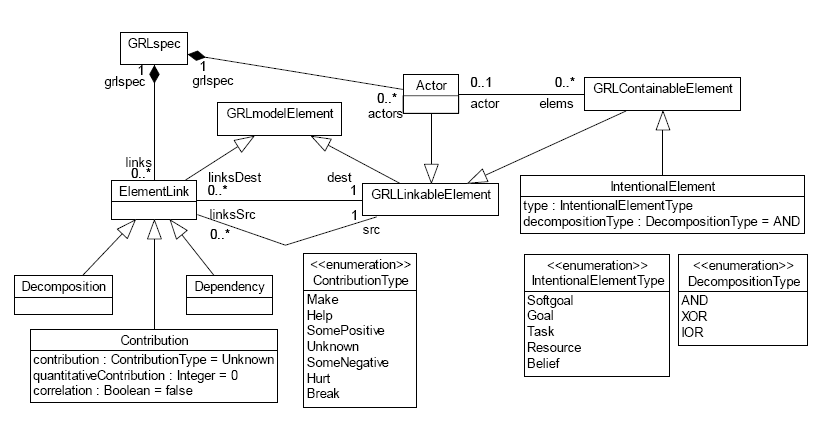
\includegraphics[width=0.95\textwidth]{grl_abstract_grammar}
\centering
\caption[GRL Abstract Grammar]{GRL Abstract Grammar defined in~\citefield{ituZ151}{journaltitle}}
\label{fig:grl_abstract_grammar}
\end{figure}

A GRL goal graph is a connected graph of intentional elements that optionally reside within an actor. The one shown in figure~\ref{fig:WirelessIN_Integrated_GRLGraph} targets the evaluation of an architectural decision about where to put the data and the logic of the authorization service of a wireless system~\citep{amyot2011user}.

\begin{figure}[h]
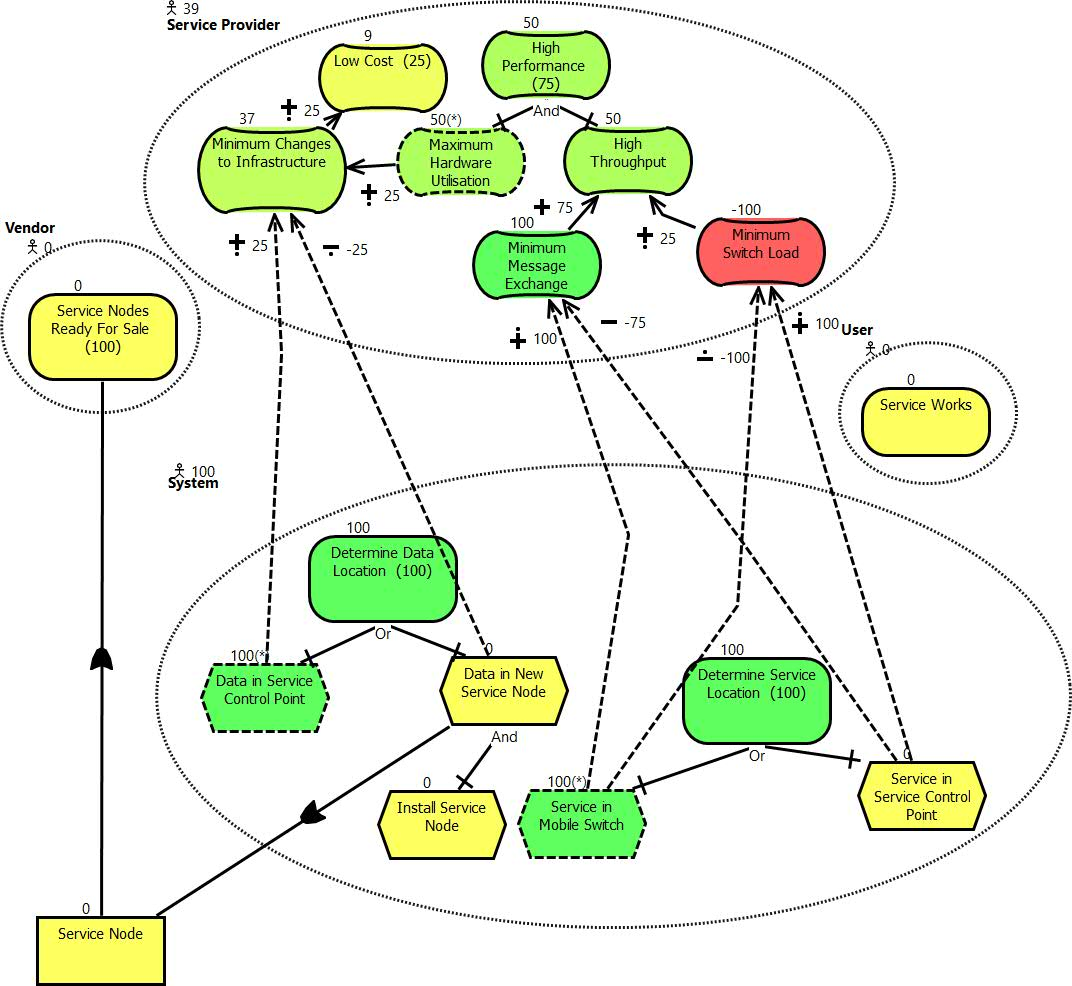
\includegraphics[width=0.85\textwidth]{WirelessIN-Integrated-GRLGraph}
\centering
\caption[Example of a GRL graph model]{Example of a GRL graph model~\citep{amyot2011user}}
\label{fig:WirelessIN_Integrated_GRLGraph}
\end{figure}

A goal graph, such as the one in figure~\ref{fig:WirelessIN_Integrated_GRLGraph}, shows the non-functional requirements and business goals of interest to the system and its stakeholders, as well as the alternatives for achieving these high-level elements. 

Figure~\ref{fig:WirelessIN_Integrated_GRLGraph} shows a particular configuration of alternatives (indicated by a star (*) and a dashed outline), consisting of assigning an initial qualitative satisfaction level of \emph{satisficed} to service control point for data location and mobile switch for service location, and the impact this decision has on the satisfaction levels of stakeholders, namely the system and service provider and their goals. Note that the algorithm used in figure~\ref{fig:WirelessIN_Integrated_GRLGraph} combined qualitative and quantitative contributions and the numbers (between -100 and 100) are a quantitative measure of the satisfaction levels of goals and stakeholders. It can be seen that, the strategy chosen resulted in a a satisfaction level for the service provider measured at 39, while the system obtained 100. Accordingly, the goals of the system have been fully satisficed whilst the ones of the service provider have only been partially or in GRL terminology, weakly satisficed. Interestingly, in spite of minimum switch load, a softgoal of the service provider being denied, the impact of that decision on high throughput was low as high throughput had been decomposed in two softgoals and minimum message exchange was satisficed fully. 

GRL defines the following qualitative contribution levels as standard (their equivalent quantitative contribution is also shown)
\begin{description}
\item[Make] 100
\item[Some Positive] 75
\item[Help] 25
\item[Unknown] 0
\item[Hurt] -25
\item[Some Negative] -75
\item[Break] -100
\end{description}

This evaluation mechanism propagates low-level decisions regarding alternatives to satisfaction ratings of high-level stakeholder goals and softgoals. GRL strategies can be compared with each other to help reach the most appropriate trade-offs among often conflicting goals of stakeholders. Colour coding of the intentional elements also reflect their satisfaction level (the greener, the more satisfied)~\citep{amyot2011user}.

\subsection{Summary}

In this chapter we have reviewed the notion of non-functional requirements and the multiple classification and representation schemes available. We followed with expanding on the importance of goals and goal-oriented approaches in the elicitation, analysis and modelling of stakeholders requirements, and in particular, quality attributes of the systems and applications that will help stakeholders attain those goals. Finally, we introduced GRL, by describing two other languages from which it spawn from, namely the \emph{NFR Framework} and \emph{i*}. While describing GRL, we focused on explaining how it supports reasoning about goals and requirements, while showing the impact of proposed alternative solutions to achieve those goals.

In the following chapters, we will introduce goal-oriented ideas and concepts in behaviour-driven development (BDD) and in doing so, offer a treatment of \nfrs as a first-class concept in BDD.

}
\chapter{Extending BDD - A goal oriented approach}
\label{ch:Extendingbdd}
In previous chapters we have presented definitions of requirements and requirements engineering, paying particular attention to the practices, concerning requirements elicitation, analysis, specification and validation found in most agile development methods, and BDD in particular.

We share the view that goal-oriented analysis complements and strengthens traditional requirements engineering techniques by offering a mechanism for capturing and evaluating alternative ways of meeting high-level goals~\citep{MylopoulosExpl2001}.

Eliciting high level goals early in the development process is crucial. However, goal-oriented requirements elicitation is an activity that continues as development proceeds, as high-level goals (such as business goals) are refined into lower-level goals (such as technical goals that are eventually operationalised in a system). Eliciting goals focuses the requirements engineer on the problem domain and the needs of the stakeholders, rather than on possible solutions to those problems~\citep{Nuseibeh:2000ub}. In addition, the requirements engineer needs to explore alternatives and evaluate their feasibility and desirability with respect to business goals.

This focus on the needs of stakeholders, even if logical and beneficial, has lead to other goals, such as cross-cutting concerns or quality concerns of stakeholders, being neglected or addressed later in the software life-cycle. In fact, incorporating these goal types, such as \nfrs, into the different phases of the software life-cycle is a very hard task. Researchers face many challenges including their great diversity,  subjective nature, difficulty in formalisation, incorporating these requirements into models used for specifying functional requirements and resolving conflicts among \nfrs~\citep{Matoussi:2008wr}. Behaviour-driven development is one such model, traditionally used for specifying functional requirements and where their non-functional counterparts are rarely given the same relevance. 

In this chapter we present, through data publicly available, a case study applying our extension to BDD that include the treatment of \nfrs as first class citizens, alongside functional requirements. Moreover, our approach is independent of the particular taxonomy chosen and remains faithful to the principles of agile development discussed in earlier chapters. 

The next chapter will focus on the changes made to Gherkin to support our methodology and also, detail a translator from feature files specified in Gherkin to GRL.

\section{Methodology}
We may be overusing the word methodology, given that some authors consider BDD not to be a methodology in its own right~\citep{Smart201410}. The extension we are proposing to BDD does not make it a full blown methodology (e.g. we are mostly silent regarding management of requirements using BDD) but it is useful to refer to our collection of methods and techniques using one word other than BDD, hence the choice for \emph{methodology}.

There are not that many references in the literature for approaches to handling non-functional requirements in agile methods and the ones that we have found are consistent with one another.~\citet{Davies} defends that agile teams should take responsibility for eliciting non-functional requirements and they should do it early-on by discussing with users the capabilities of the system, like quality of service and longevity, at the start of the project. The author is of the opinion, there are three approaches to describe these required capabilities in agile methods. Some teams like to use the usual story format (see listing~\ref{lst:story_template}) as in this way, all requirements look the same, can be understood by everyone including non-technical individuals, and therefore have the same visibility as other stories. Other teams keep it simple and simply factor \nfrs into acceptance criteria for affected user stories. Finally, last approach is to introduce `technical stories' to cover anything that needs to be built or restructured but is too difficult to explain to business people. These story cards are typically free format and expressed in a language that only the development team understands~\citep{Davies}.

\begin{center}
\begin{description}
\item[As a] \textless Role \textgreater
\item[I want] \textless Goal \textgreater
\item[So that] \textless Benefit \textgreater
\end{description}
\end{center}

\citet{CohnNFRS} advises the use of the story format and gives examples where, in his view, non-functional characteristics can be expressed using the template above

\begin{center}
\begin{description}
\item[As a] CTO 
\item[I want] the system to use our existing orders database rather than create a new one
\item[So that] we don't have one more database to maintain
\end{description}
\end{center}

or

\begin{center}
\begin{description}
\item[As a] user
\item[I want] the site to be available 99.999 percent of the time I try to access it
\item[So that] I don't get frustrated and find another site to use
\end{description}
\end{center}

Trying to write \nfrs in this template is a good exercise, as it helps make sure we understand who wants what and why, as the above examples demonstrate. \citet{CohnNFRS} points out though that we should pay attention not to get obsessed with this format and instead specify it in whatever way feels natural, if using the template leads to confusingly formed sentences.

In our research, we found the user story format appropriate to write both functional and non-functional requirements. Our extension to Gherkin requires writing requirements in user story format, as we need to differentiate the goal from the stakeholder/role it intends to benefit. We do not believe this to be a significant drawback, but it does represent a breaking change with existing feature files. A small refactoring to the extended Gherkin parser described in chapter~\ref{ch:gherkin_redux} would satisfy this requirement.

In this work, we use the approach of~\citet{Chung:2009vg} of considering as non-functional requirements, any `-ilities', `-ities', such as usability or security, along with many other things that do not necessarily end with either of them, such as performance or user-friendliness. In view of mathematical functions, in the form of, $\mathit{function} : \mathit{Input} \rightarrow \mathit{Output}$, just about anything that addresses characteristics of a function, a function's input or output or relationships between the two, can be considered as non-functional requirement.

\citet{Leffingwell2011} identifies, together with functional and non-functional requirements, design constraints as another class of requirements (see table~\ref{tb:three_req_types}). Design constraints typically originate from one of three sources: some necessary restriction of design options, conditions imposed on the development process itself, and regulations and imposed standards.\fxnote{Argument in conclusion}

\begin{table}[h!]
\caption[Three types of Requirements]{Three types of requirements~\citep{Leffingwell2011}}
\label{tb:three_req_types}
\setlength{\extrarowheight}{1.8pt}
\centering
\scalebox{0.75}{
\begin{tabularx}{\textwidth}{cX}
\toprule \multicolumn{1}{c}{\bfseries{Requirement Type}}&
\multicolumn{1}{c}{\bfseries{Description}}\\
\addlinespace
\midrule
Functional requirements & Express how the system interacts with its users-its inputs, its outputs, and the functions and features it provides \\ \midrule
Non-functional requirements &  Criteria used to judge the operation or qualities of a system \\ \midrule
Design constraints & Restrictions on the design of a system, or the process by which a system is developed, but that must be fulfilled to meet technical, business, or contractual obligations \\
\addlinespace
\bottomrule
\end{tabularx}
}
\end{table}

Our approach integrates all of the above requirements in a coherent manner, where both non-functional requirements and design constraints are treated as softgoals that can be specified alongside functional requirements. In extending BDD, our research aimed at integrating goal-reasoning concepts, while being shaped by the philosophy and principles of agile development. In other words, we extend BDD by 

\begin{itemize}
\item following a lightweight approach
\item requiring minimal changes to Gherkin
\item preventing subversion of the spirit behind \emph{Specification by Example}
\item respecting the strengths of BDD and GRL
\item following a separation of concerns policy when integrating Gherkin and GRL
\end{itemize}

In what follows, we will be assuming an iterative development approach, even though the description of the steps involved will be sequential. That is the nature of writing, and more so when documenting the results of technical research. We use a similar approach as~\citet{Chung2000} of following a process of developing a target artefact by starting with a source specification and producing constraints upon the target artefact. This could occur at various phases of development (e.g., requirements specification, conceptual design, or development).

The \emph{NFR Framework} uses non-functional requirements such as security, accuracy, performance and cost to drive the overall design process~\citep{Chung2000}. BDD in turn, uses expected behaviours of a system to drive the development process. We assume a hybrid approach, by retaining its behaviour-driven characteristics, but adding constrains derived from non-functional requirements.
\clearpage

Analogously to the \emph{NFR Framework}, there are several major steps in this process:
\begin{itemize}
\item acquiring or accessing knowledge of the particular domain and the system which is being developed, functional requirements for the particular system, and particular kinds of NFRs, and associated development techniques
\item identifying particular NFRs for the domain
\item decomposing NFRs,
\item deducing `operationalisations' (possible design alternatives for meeting NFRs in the target system)
\item dealing with ambiguities, trade-offs and priorities, and interdependencies among NFRs and operationalizations
\item selecting operationalisations
\item supporting decisions with design rationale
\item evaluating the impact of decisions.
\end{itemize}

Again, these steps are not followed in sequence and we do not intend to introduce each, one at a time. It will hopefully be clear from the presentation, what each step consists of and when it is being applied. 
In presenting our results and describing our methodology, we will make use of case study data contained on the \emph{PROMISE}~(Predictor Models in Software Engineering) requirements dataset~(\emph{PROMISE}, 2015). The \emph{PROMISE} dataset consists of 625 requirements collected from 15 software development projects. Among them, 255 items are marked as functional requirements and the remaining 370 non-functional requirements items are classified into 11 categories, such as Security, Performance and Usability.

One of the projects included in the dataset, is a \emph{meeting scheduler}. Functionally, the \emph{meeting scheduler} is required to create meetings, send invitations, book conference rooms, book room equipment and so on. Table~\ref{tb:scheduler_original_frs} lists all original functional requirements  contained in the dataset. Note that to facilitate tracing to the original \emph{PROMISE} dataset we are retaining the requirements identifiers used therein.

\ifdraft{%
  \fxnote{THIS WILL CONTAIN FRs TABLE for CASE STUDY}
}{%
\begin{table}[h!]
\caption[Meeting scheduler original functional requirements]{Meeting scheduler original functional requirements~(\emph{PROMISE}, 2015)}
\label{tb:scheduler_original_frs}
\setlength{\extrarowheight}{1.8pt}
\centering
\scalebox{0.85}{
\begin{tabularx}{\textwidth}{cX}
    \toprule \multicolumn{1}{c}{\bfseries{Requirement ID}}&
    \multicolumn{1}{c}{\bfseries{Functional Requirement Description}}\\
    \addlinespace
    \midrule
    R 48  & The product shall record meeting entries \\ \midrule
    R 49  & The product will notify employees of meeting invitations \\ \midrule
    R 50  & The product shall have the ability to send meeting reminders to employees \\ \midrule
    R 51  & The product shall assign the organizers contact information to each meeting they create \\ \midrule
    R 52  & The product will record meeting acknowledgements \\ \midrule
    R 53  & The product shall store new conference rooms \\ \midrule
    R 54  & The product shall update existing conference rooms \\ \midrule
    R 55  & The product will be able to delete conference rooms \\ \midrule
    R 56  & The product shall be able to store new room equipment \\ \midrule
    R 57  & The product will update existing room equipment \\ \midrule
    R 58  & The product shall be able to delete room equipment \\ \midrule
    R 59  & The product shall allow an organizer to invite other employees to meetings \\ \midrule
    R 60  & Each time a conference room is reserved the conference room schedule shall be updated to reflect the time and date of the reservation \\ \midrule
    R 61  & The product shall record the transportation status of equipment reserved \\ \midrule
    R 62  & The product shall display a map of the company building showing conference room locations \\ \midrule
    R 63  & The product shall record updated meeting agendas \\ \midrule
    R 64  & The product shall send a meeting confirmation to the meeting organizer \\ \midrule
    R 65  & The product shall display room equipment according to search parameters \\ \midrule
    R 66  & The product shall display conference rooms according to search parameters \\ \midrule
    R 67  & The product shall record different meeting types \\ \midrule
    R 68  & The product shall record all the equipment that has been reserved \\ \midrule
    R 69  & The product shall notify building personnel of equipment transport requests \\ \midrule
    R 70  & The product will allow privileged users to view meeting schedules in multiple reporting views \\ \midrule
    R 71  & The product shall be able to send meeting notifications via different kinds of end-user specified methods \\ \midrule
    R 72  & The product shall have a customizable Look and Feel \\ \midrule
    R 73  & The product shall have an intuitive user interface \\ \midrule
    R 74  & The product will display an available status for unreserved conference rooms \\
    \addlinespace
    \bottomrule
    \end{tabularx}
}
\end{table}
}

The case study example includes 27 functional requirements and 47 \nfrs, covering different aspects of the system, such as interoperability, usability, security, user friendliness, etc. The entire list of original non-functional requirements of the \emph{meeting scheduler} case study can be found in Appendix~\ref{ch:case_study_appendix}. 

The dataset also specifies for each non-functional requirement if it traces to a functional requirement, that is if that functional requirement is impacted by the non-functional requirement. That mapping is presented in table~\ref{tb:scheduler_original_frs_to_nfrs} (the absence of a particular non-functional requirement identifier from the columns of the table, implies there is no dependency between that non-functional and any of the functional requirements)

\ifdraft{%
  \fxnote{THIS WILL CONTAIN FRS to NFRS MAPPING TABLE}
}{%
\begin{table}[h!]
\caption[Meeting scheduler mapping of functional to non-functional requirements]{Meeting scheduler mapping of functional to non-functional requirements~(\emph{PROMISE}, 2015)}
\label{tb:scheduler_original_frs_to_nfrs}
\setlength{\extrarowheight}{1.8pt}
\centering
\scalebox{0.75}{
    \begin{tabular}{rrccccccccccccccccccccccccccccccccccccccccccccccc}
    \toprule
              & \multicolumn{11}{c}{\bfseries{Non-Functional Requirements}} \\
        \midrule
        \multicolumn{1}{c}{\bfseries{Req ID}} & \begin{turn}{45}R 138\end{turn} & \begin{turn}{45}R 140 (*)\end{turn} & \begin{turn}{45}R 142 (*)\end{turn} & \begin{turn}{45}R 146\end{turn} & \begin{turn}{45}R 149\end{turn} & \begin{turn}{45}R 152\end{turn} & \begin{turn}{45}R 162\end{turn} & \begin{turn}{45}R 163\end{turn} & \begin{turn}{45}R 168\end{turn} & \begin{turn}{45}R 178\end{turn} & \begin{turn}{45}\end{turn} \\
            \multicolumn{1}{c}{R 48} & \multicolumn{1}{l}{I}     & \multicolumn{1}{l}{I}     & \multicolumn{1}{l}{I}     &       &       &       & \multicolumn{1}{l}{I}     &       &       &       & \multirow{27}[54]{*}{} \\
            \multicolumn{1}{c}{R 49} & \multicolumn{10}{c}{\multirow{4}[8]{*}{}}                                     &  \\
            \multicolumn{1}{c}{R 50} & \multicolumn{10}{c}{}                                                         &  \\
            \multicolumn{1}{c}{R 51} & \multicolumn{10}{c}{}                                                         &  \\
            \multicolumn{1}{c}{R 52} & \multicolumn{10}{c}{}                                                         &  \\
            \multicolumn{1}{c}{R 53} & \multicolumn{1}{l}{I}     & \multicolumn{1}{l}{I}     & \multicolumn{1}{l}{I}     &       &       &       & \multicolumn{1}{l}{I}     &       &       &       &  \\
            \multicolumn{1}{c}{R 54} & \multicolumn{1}{l}{I}     & \multicolumn{1}{l}{I}     & \multicolumn{1}{l}{I}     &       &       &       & \multicolumn{1}{l}{I}     &       &       &       &  \\
            \multicolumn{1}{c}{R 55} & \multicolumn{1}{l}{I}     & \multicolumn{1}{l}{I}     & \multicolumn{1}{l}{I}     &       &       &       & \multicolumn{1}{l}{I}     &       &       &       &  \\
            \multicolumn{1}{c}{R 56} & \multicolumn{1}{l}{I}     & \multicolumn{1}{l}{I}     & \multicolumn{1}{l}{I}     &       &       &       & \multicolumn{1}{l}{I}     &       &       &       &  \\
            \multicolumn{1}{c}{R 57} & \multicolumn{1}{l}{I}     & \multicolumn{1}{l}{I}     & \multicolumn{1}{l}{I}     &       &       &       & \multicolumn{1}{l}{I}     &       &       &       &  \\
            \multicolumn{1}{c}{R 58} & \multicolumn{1}{l}{I}     & \multicolumn{1}{l}{I}     & \multicolumn{1}{l}{I}     &       &       &       & \multicolumn{1}{l}{I}     &       &       &       &  \\
            \multicolumn{1}{c}{R 59} & \multicolumn{10}{c}{}                                                         &  \\
            \multicolumn{1}{c}{R 60} &       &       &       & \multicolumn{1}{l}{O,P}   &       &       &       &       &       & \multicolumn{1}{l}{O}     &  \\
            \multicolumn{1}{c}{R 61} & \multicolumn{1}{l}{I}     & \multicolumn{1}{l}{I}     & \multicolumn{1}{l}{I}     &       &       &       & \multicolumn{1}{l}{I}     &       &       &       &  \\
            \multicolumn{1}{c}{R 62} &       &       &       &       &       & \multicolumn{1}{l}{L}     &       &       & \multicolumn{1}{l}{MA,MO} &       &  \\
            \multicolumn{1}{c}{R 63} & \multicolumn{1}{l}{I}     & \multicolumn{1}{l}{I}     & \multicolumn{1}{l}{I}     &       &       &       & \multicolumn{1}{l}{I}     &       &       &       &  \\
            \multicolumn{1}{c}{R 64} &       &       &       &       &       &       &       & \multicolumn{1}{l}{I}     &       &       &  \\
            \multicolumn{1}{c}{R 65} & \multicolumn{10}{c}{\multirow{2}[4]{*}{}}                                     &  \\
            \multicolumn{1}{c}{R 66} & \multicolumn{10}{c}{}                                                         &  \\
            \multicolumn{1}{c}{R 67} & \multicolumn{1}{l}{I}     & \multicolumn{1}{l}{I}     & \multicolumn{1}{l}{I}     &       &       &       & \multicolumn{1}{l}{I}     &       &       &       &  \\
            \multicolumn{1}{c}{R 68} & \multicolumn{1}{l}{I}     & \multicolumn{1}{l}{I}     & \multicolumn{1}{l}{I}     &       &       &       & \multicolumn{1}{l}{I}     &       &       &       &  \\
            \multicolumn{1}{c}{R 69} & \multicolumn{10}{c}{}                                                         &  \\
            \multicolumn{1}{c}{R 70} & \multicolumn{1}{l}{I}     & \multicolumn{1}{l}{I}     & \multicolumn{1}{l}{I}     &       & \multicolumn{1}{l}{AS}    &       & \multicolumn{1}{l}{I}     &       &       &       &  \\
            \multicolumn{1}{c}{R 71} &       &       &       &       &       &       &       & \multicolumn{1}{l}{I}     &       &       &  \\
            \multicolumn{1}{c}{R 72} &       &       &       &       & \multicolumn{1}{l}{AS}    &       &       &       &       &       &  \\
            \multicolumn{1}{c}{R 73} &       &       &       &       & \multicolumn{1}{l}{L,AS}  &       &       &       &       &       &  \\
            \multicolumn{1}{c}{R 74} &       &       &       & \multicolumn{1}{l}{O,P}   &       & \multicolumn{1}{l}{L}     &       &       &       &       &  \\
        \bottomrule
    \end{tabular}%
}
\caption*{
        \scalebox{0.85}{
            \begin{tabular}{c c l}
              \multicolumn{1}{c}{\multirow{3}[1]{*}{\emph{\bfseries{Legend:}} In the above, initials represent qualities}} 
                & O	 & Operability \\
                & P	 & Pleasure \\
                & I	 & Interoperability \\
                & L	 & Learnability \\
                & MA & Maintainability \\
                & MO & Modifiability \\
                & AS & user interface aesthetics \\
                \multicolumn{2}{c}{\multirow{3}[1]{*}{\emph{\bfseries{(*)}} \citet{MylopoulosOnt2014} marked these as Functional requirements and we will not consider them}} 
            \end{tabular}
        }
  }
\end{table}
}

We were unsatisfied with the choice of taxonomy used in the dataset, as the data contains no guidance or indication is this respect. Also, some of the categorisations used were arguably inconsistent. For example, functional requirement 48 is originally impacted by non-functional requirements 138, 140, 142 and 162 and all of these have been categorised as Operational, whilst in our view 138 and 140 are more pertinent to interoperability constraints and 142 is more of a design constraint, rather than a specific non-functional requirement.

We also took into consideration an ontological approach and analysis done to this case study dataset~\citep{MylopoulosOnt2014}. Their classification includes three basic categories of requirements, `functional requirement (FR)', `quality requirement (QR)', and `constraints over function (CF)'. These would be modelled by functional goals, quality goals and function constraints in their conceptual model. They have also identified an additional category, `Domain Assumption' that, in their words, can operationalise any other goal.

The authors analysed the 47 \nfrs within the dataset, and identified 21 QRs, 9 FRs, 14 Qrs+FRs, 2 CF+QR, and 1 DA. In the interest of space, we have decided to ignore any non-functional requirement that has been identified as FR, given that treating these would have no other consequence than growing our list of functional requirements to address. Therefore, and for the above reason, requirements 140 and 142 would fall from our list of \nfrs to take into consideration.

In this context, we opted by using the categorization in~\citefield{ieee_std_25010}{journaltitle}, and reproduced again in figure~\ref{fig:iso25010_again} for easy referencing.

\captionsetup[figure]{list=no}
\begin{figure}[h!]
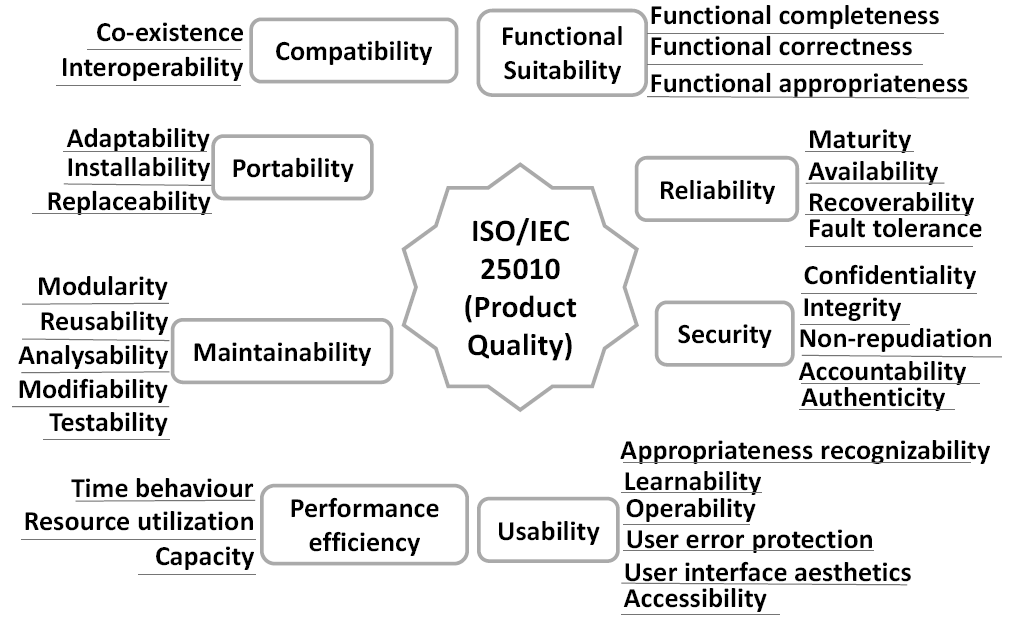
\includegraphics[width=0.65\textwidth]{iso25010}
\centering
\caption[ISO 25010 quality model]{ISO 25010 quality model in ~\citefield{ieee_std_25010}{journaltitle}}
\label{fig:iso25010_again}
\end{figure}
\captionsetup[figure]{list=yes}

Therefore, in what follows, we use 10 \nfrs (the ones that impact one or more of the functional requirements), with the meaning intended by Leffingwell, that is, requirements that define criteria used to judge the operation or qualities of a system~\citep{Leffingwell2011}. Other requirements, listed originally as non-functional requirements, fall in the category of design constraints, such as requirements with identifiers 139, \emph{`The product will function alongside server software on any operating system where the Java runtime can be installed'} or 141, \emph{`The product must make use of web/application server technology. Open source examples include Apache web server Tomcat and the JBoss application server'}. 

In the interest of space and keeping discussion relevant, we will address all three types of requirements, that is functional, non-functional and design constraints, but will devote more attention to the requirements contained in the mapping table~\ref{tb:scheduler_original_frs_to_nfrs}. The reasons for this will become clear when we describe our extended format for feature files, as in our methodology, design constraints are addressed no differently than non-functional requirements with a global reach, one that causes them to have an impact on all other goals.

Before describing how we model this set of requirements using our extended BDD methodology, we need to surface some constraints that we were faced with and that shaped our approach. We had to assume that the list of requirements was consistent with original goals of the stakeholders, whoever they may be. This was the first hurdle we had to overcome, and that was identifying the different stakeholders of the system. Note that it was not our intention to identify all possible stakeholders, but rather only the ones that could be derived from the dataset.

We note also, that we did not have access to stakeholders and could not confirm assumptions, refine requirements or deal with ambiguities, or had access to business users from whom we could obtain further knowledge about the domain. This is not to say that we cannot use our methodology with confidence, it is just that we need to be appreciative of the constrained context in which our research took place.

In other words, our focus is on proving the feasibility (or not, for that matter) of our approach and to present the benefits, challenges and conclusions of our research. It is not to design the best possible \emph{meeting scheduler} given a set of elicited requirements. That would just not be possible without a significant amount of guess work. 

Figure~\ref{fig:gherkin_ast} contains a class model of the current Gherkin implementation. At the centre of the model are \emph{Features}, consisting of a name, a description, an optional list of tags and comments, and a list of \emph{Scenario Definitions} with an optional \emph{Background}. A name is synonymous with title, and description is a block of text in no particular format. \emph{Keyword} is filled by the parser and represents what lexeme was parsed (e.g. for a feature, one can use `Feature', `Business Need' or `Ability') when processing each line of a feature file. \emph{Background} adds context to the scenarios in a single feature and is similar to a scenario containing a number of \emph{Steps}. \emph{Tags} can be used to group features and scenarios together. Every \emph{scenario} consists of a list of \emph{Steps}, which must start with one of the keywords \emph{Given}, \emph{When}, \emph{Then}, \emph{But} or \emph{And}. These \emph{Steps}, are the interface to external tools to support testing and automated test execution approaches.

In the next section, we will introduce our changes to Gherkin by using a subset of requirements from the \emph{meeting scheduler} case study.

\section{Meeting scheduler case study}
\label{sec:case_study}
Based on the set of functional requirements (see table \ref{tb:scheduler_original_frs}) we devised the following list of stakeholders

\begin{description}
\item[\emph{Procurement Manager}] \hfill \\
Represents the concerns and interests of those that select, purchase and buy software
\item[\emph{Privileged User}] \hfill \\
Represents a user that due to reasons of seniority or others, has privileged access to a service or application
\item[\emph{Meeting Organiser}] \hfill
Represents the concerns and interests of those users that want to organise meetings
\item[\emph{Facilities Manager}] \hfill \\ 
Represents those individuals that are responsible for the security, maintenance and services of work facilities to ensure that they meet the needs of the organisation and its employees
\end{description}

When addressing each requirement we determined which stakeholder does the requirement pertain to. While there may be multiple stakeholders impacted by the requirement, in our approach only one of them will have the requirement assigned to. This is a current limitation of our approach, even though for most practical purposes, and without loss of generality, each goal usually pertains to at most one stakeholder.
 
In order to describe changes to Gherkin we will make use of a subset of requirements from the \emph{meeting scheduler} case study. This subset of requirements is listed below

\begin{table}[h!]
\caption[Exemplar subset of meeting scheduler requirements]{Exemplar subset of meeting scheduler requirements}
\label{tb:case_study_reqs_for_analysis}
\setlength{\extrarowheight}{1.8pt}
\centering
\scalebox{0.85}{
\begin{tabularx}{\textwidth}{cX}
\toprule \multicolumn{1}{c}{\bfseries{Requirement ID}}&
\multicolumn{1}{c}{\bfseries{Requirement Description}}\\
\addlinespace
\midrule
 R 48  & The product shall record meeting entries \\ \midrule
 R 63  & The product shall record updated meeting agendas \\ \midrule
 R 67  & The product shall record different meeting types \\ \midrule
 R 73  & The product shall have an intuitive user interface \\ 
\addlinespace
\bottomrule
\end{tabularx}
}
\end{table}

The reason these requirements are of particular interest is because, requirements 63 and 67 are impacted by 48, while 73 is a global non-functional requirement, in the sense that constrains all other functional requirements, and these variations cover all of our extensions to BDD.

Starting with requirement 48, it can be argued that recording meetings is of particular interest to the \emph{Meeting Organiser} role. We then introduce our first change to Gherkin, which is being able to specify requirements in user story format.

\begin{featurelist}{Changes to Gherkin -- User story format}{lst:gherkin_changes_userstory}
\begin{featurecode}{0.7}
\begin{minted}{Gherkin}
Feature:    R48 - The product shall record meeting entries

            As a Meeting Organiser
            I want to record meeting entries
            So that I can always access a persisted record of each meeting
\end{minted}
\end{featurecode}
\end{featurelist}

We introduce the concepts of an \emph{Actor}, in this case \emph{Meeting Organiser}, representing a stakeholder or system; a \emph{Goal}, in this case \emph{record meeting entries}, representing an actor's high-level desire or need and a \emph{Benefit}, in this case \emph{I can always access a persisted record of each meeting}, which represents the anticipated benefit for an actor if the specified goal is achieved.

\emph{Actors} are extremely relevant, as they represent stakeholders that usually have different, and at times conflicting concerns, and not only those need to be addressed and conflicts resolved, but also the actor's satisfaction level, needs to be assessed.

\emph{Goals} equate very closely with functional requirements and it will be by satisfying them (and also \emph{Sofgoals}, representing non-functional requirements and addressed later) that an actor's satisfaction level can be evaluated. \emph{Benefits} are used to document the perceived benefit of achieving a goal, and help justify modelling decisions in GRL.

\emph{Actors} and \emph{Goals} are GRL concepts (see chapter~\ref{ch:nfr_research},~section~\ref{sec:gore} for details on these concepts) that will be used by a Gherkin to GRL translator that will be described in chapter~\ref{ch:gherkin_redux}. \emph{Benefits} will not be translated to GRL as we did not find a suitableGRL element to map them to.\fxnote{Mention No mapping to Benefits in Conclusion}

In order to address conflicts amongst \emph{Goals}, we extend the user story format with one or more references to other goals that may be impacted by a given goal~(see listing \ref{lst:gherkin_changes_impactedgoals}). The keyword used is \emph{Which may impact} followed by a \emph{Goal} that needs to be defined in another feature file.

\begin{featurelist}{Changes to Gherkin -- Impacted goals}{lst:gherkin_changes_impactedgoals}
\begin{featurecode}{0.7}
\begin{minted}{Gherkin}
Feature:    R48 - The product shall record meeting entries

            As a Meeting Organiser
            I want to record meeting entries
            So that I can always access a persisted record of each meeting
            Which may impact record a meeting agenda
            Which may impact record different meeting types

\end{minted}
\end{featurecode}
\end{featurelist}

The careful reader will have already identified \emph{record a meeting agenda} and \emph{record different meeting types} as the goals for requirements 63 and 67. To our knowledge, this is the first time that, in BDD practices, goals of stakeholders have been collectively addressed and potential conflicts or dependencies identified and taken into consideration. In GRL this will correspond to a \emph{Dependency} link.

If we refer to table~\ref{tb:scheduler_original_frs_to_nfrs}, that maps functional to non-functional requirements that impact them, we note that requirement 48 is constrained by an \emph{Interoperability} quality characteristic. That leads us to the next change, that is, attaching constraints to behaviours of systems or applications (see listing~\ref{lst:gherkin_changes_constraints}).

\begin{featurelist}{Changes to Gherkin -- Constraints}{lst:gherkin_changes_constraints}
\begin{featurecode}{0.7}
\begin{minted}{Gherkin}
Feature:    R48 - The product shall record meeting entries

            As a Meeting Organiser
            I want to record meeting entries
            So that I can always access a persisted record of each meeting
            Which may impact record different meeting types
            Which may impact record a meeting agenda
	
Constrained by:
            | Interoperability | Help |
\end{minted}
\end{featurecode}
\end{featurelist}

While the \emph{Feature} keyword is used to name and mark the beginning of a feature file, the keyword \emph{Constrained by} (note that \emph{Without ignoring} may also be used) lists the quality characteristics that constrain this functionality, and therefore should not be ignored. The lines immediately below are parsed as a table (using $\vert$ as a cell separator) to list the non-functional characteristics and the expected \emph{contribution} level for the satisfaction of the goal. In other words, and referring to this feature in particular, we expect Interoperability to \emph{help} (see chapter~\ref{ch:nfr_research}, section~\ref{sec:gore} for more on contribution levels) achieve the \emph{record meeting entries} goal. In GRL this will correspond to a \emph{Contribution} link.

\emph{Interoperability} is appropriate as a grouping term, but is not specific enough to support analysis. If we revert to mapping table~\ref{tb:scheduler_original_frs_to_nfrs} we can see that this requirement is impacted by four \nfrs, all related to the \emph{Interoperability} quality characteristic. Table~\ref{tb:three_nfrs_impacting_r48} lists those requirements

\captionsetup[table]{list=no}
\begin{table}[h!]
\caption{Four \nfrs impacting functional requirement 48}
\label{tb:three_nfrs_impacting_r48}
\setlength{\extrarowheight}{1.8pt}
\centering
\scalebox{0.75}{
\begin{tabularx}{\textwidth}{cX}
\toprule \multicolumn{1}{c}{\bfseries{Requirement Type}}&
\multicolumn{1}{c}{\bfseries{Description}}\\
\addlinespace
\midrule
R 138   & The product must work with most database management systems (DBMS) on the market whether the DBMS is colocated with the product on the same machine or is located on a different machine on the computer network. \\ \midrule
R 140   & The product will require collaboration with a database management system (DBMS). The DBMS may be located on the same machine as the product or on a separate machine residing on the same computer network. \\    \midrule
R 142   & A database management system such as Oracle DB2 MySql or HSQL will need to be integrated with the product \\ \midrule
R 162   & The product must be able to interface with various database management systems. The product shall communicate successfully with the database management system on 100\textbackslash{}\% of all transactions. \\
\addlinespace
\bottomrule
\end{tabularx}
}
\end{table}
\captionsetup[table]{list=yes}

As we mentioned before, 140 and 142 have been considered to be functional requirements~\citep{MylopoulosOnt2014} and therefore, will not receive our attention as they would need to be addressed in separate feature files and would complicate this description process further. We are then left with requirements with identifiers 138 and 162.

In BDD, and in the spirit of \emph{Specification by Example}, we clarify requirements details through examples and these, in the context of feature files, are represented by \emph{Scenarios}. Listing~\ref{lst:gherkin_changes_scenarios} shows the revised feature file

\begin{featurelist}{Changes to Gherkin -- Scenarios}{lst:gherkin_changes_scenarios}
\begin{featurecode}{0.7}
\begin{minted}{Gherkin}
Feature:    R48 - The product shall record meeting entries

            As a Meeting Organiser
            I want to record meeting entries
            So that I can always access a persisted record of each meeting
            Which may impact record different meeting types
            Which may impact record a meeting agenda
	
Constrained by:
            | Interoperability | Help |

@NFR
Scenario:   Meeting entries can be recorded in most DBMS
            Which helps Interoperability

@NFR	
Scenario:   100% of all transactions recording meeting entries in DBMS are successful
            Which helps Interoperability

Scenario:   Record simplest meeting
            Given the application has been started
            And I choose to add new meeting
            When I specify a meeting name and date
            And I proceed to save the meeting
            Then the meeting should be recorded
\end{minted}
\end{featurecode}
\end{featurelist}

Note that the two first scenarios are tagged with the tag \emph{\@NFR} to indicate they are examples of a non-functional characteristic. We also state the \emph{Contribution} level (\emph{Help}) of each particular scenario to the attainment of the quality desired, in this case, \emph{Interoperability}. We believe this communicates better what behaviour is expected from the system than taking the individual requirements 138 and 162 on their own. The latter option, made them slightly confusing as they seemed to overlap to some extent and were unrelated, where in fact they constrain the same functionality and contribute to attain the same \emph{Interoperability} quality.

We are also listing a third scenario, \emph{Record simplest meeting}, which is an ordinary BDD example detailing the expected behaviour of this feature. Because we are modelling behaviours using Goals, and in this particular case, the Goal is to \emph{record meeting entries}, this is equivalent of saying that \emph{Record simplest meeting}, if satisficed, contributes to the satisfaction of \emph{record meeting entries}. We have set an assumption, that if no contribution level is specified -- as in this case --, then a default contribution \emph{Help} level shall be used.

In GRL, we will use \emph{Tasks} to represent scenarios and the two situations described above are modelled using \emph{Contributions}, from \emph{Task} to \emph{Softgoal} in the first situation, and from \emph{Task} to \emph{Goal} in the second.\\

The complete feature file is listed below with remaining scenarios included.

\begin{featurelist}{Changes to Gherkin -- Complete 48 feature}{lst:gherkin_changes_complete}
\begin{featurecode}{0.7}
\begin{minted}{Gherkin}
Feature:    R48 - The product shall record meeting entries

            As a Meeting Organiser
            I want to record meeting entries
            So that I can always access a persisted record of each meeting
            Which may impact record different meeting types
            Which may impact record a meeting agenda
	
Constrained by:
            | Interoperability | Help |

@NFR
Scenario:   Meeting entries can be recorded in most DBMS
            Which helps Interoperability

@NFR	
Scenario:   100% of all transactions recording meeting entries in DBMS are successful
            Which helps Interoperability
	
Scenario:   Record simplest meeting
            Given the application has been started
            And I choose to add new meeting
            When I specify a meeting name and date
            And I proceed to save the meeting
            Then the meeting should be recorded
	
Scenario:   Record meeting for a date in the past fails with a warning to the user
            Given the application has been started
            And I choose to add new meeting
            When I specify a date in the past
            And I proceed to save the meeting
            Then the meeting should not be recorded
            And the user is warned with an appropriate message
            Which helps record meeting entries

Scenario:   Record complex meeting
            Given the application has been started
            And I choose to add new meeting
            When I specify a meeting with 10 attendants
            And I choose an available conference room
            And I request a projector to be available
            And I proceed to save the meeting
            Then the meeting should be recorded
            With some positive contribution to record meeting entries
            Contributing to help Interoperability
\end{minted}
\end{featurecode}
\end{featurelist}

A last point to make regarding this feature, is that it is possible to specify, for the same scenario, contributions to both the feature's goal and one or more quality characteristics (refer to scenario \emph{Record complex meeting}). Note that, on these occasions, the scenario should not be tagged with \emph{NFR} as it is not an example of a quality requirement only, but rather an example of a feature's goal that also happens to contribute to attain a quality characteristic.

The remaining features, corresponding to requirements with identifiers 63 and 67 can be found in listings \ref{lst:feature_r63} and \ref{lst:feature_r67}.

\begin{featurelist}{R63 -- The product shall record updated meeting agendas}{lst:feature_r63}
\begin{featurecode}{0.7}
\begin{minted}{Gherkin}
Feature:    R63 - The product shall record updated meeting agendas

            As a Meeting Organiser
            I want to record a meeting agenda
            So that I can have access to the details of the meeting
	
Constrained by:
            | Interoperability | Help |

Scenario:   Record meeting agenda with details in text

Scenario:   Record meeting agenda with details in HTML

@NFR	
Scenario:   Meeting agendas can be recorded in most DBMS
            Which helps Interoperability

@NFR	
Scenario:   100% of all transactions recording meeting agendas in DBMS are successful
            Which helps Interoperability
\end{minted}
\end{featurecode}
\end{featurelist}

\begin{featurelist}{R67 -- The product shall record different meeting types}{lst:feature_r67}
\begin{featurecode}{0.7}
\begin{minted}{Gherkin}
Feature:    R67 - The product shall record different meeting types

            As a Meeting Organiser
            I want to record different meeting types
            So that I can chose the most appropriate type of meeting
	
Constrained by:
            | Interoperability | Help |

Scenario:   Record one to one meeting

Scenario:   Record team meeting
	
@NFR	
Scenario:   Different Meeting types can be recorded in most DBMS
            Which helps Interoperability

@NFR
Scenario:   100% of all transactions recording different meeting \
            types in DBMS are successful
            Which helps Interoperability
\end{minted}
\end{featurecode}
\end{featurelist}

The last requirement to address is the one with identifier 73, and by doing so, we will introduce our last change to Gherkin and that is allowing the specification of global \nfrs or design constraints. For easy reference, we list requirement 73 and \nfrs it is impacted by, in table~\ref{tb:case_study_cross_cutting}

\begin{table}[h!]
\caption[Cross-cutting \nfrs]{Cross-cutting \nfrs}
\label{tb:case_study_cross_cutting}
\setlength{\extrarowheight}{1.8pt}
\centering
\scalebox{0.85}{
\begin{tabularx}{\textwidth}{cX}
\toprule \multicolumn{1}{c}{\bfseries{Requirement ID}}&
\multicolumn{1}{c}{\bfseries{Requirement Description}}\\
\addlinespace
\midrule
 R 73  & The product shall have an intuitive user interface \\ \midrule
 R 149 & The product shall allow for customization of start page and views preferences \\
\addlinespace
\bottomrule
\end{tabularx}
}
\end{table}

Note that this feature, also introduces a new actor, namely \emph{Procurement Manager} as we decided to model this cross-cutting concern as a goal of a stakeholder that carries that overall interest in the application's user interface and learnability characteristics. This learnability quality requirement is not something that was part of the original dataset, but a quality that we derived from our interpretation of the requirements.

\begin{featurelist}{R73 -- The product shall have an intuitive user interface}{lst:feature_r73}
\begin{featurecode}{0.7}
\begin{minted}{Gherkin}
Feature:  R73 - The product shall have an intuitive user interface
			
            @GLOBAL
            As a Procurement Manager
            I want the product to have an intuitive interface
            So that all users are able to use the product without difficulty
	
Constrained by:
            | user interface aesthetics | Help	 |
            | Learnability	      | SomePositive |
		
@NFR		
Scenario:   Product has an intuitive interface
            Which makes user interface aesthetics
            Contributing to make Learnability
\end{minted}
\end{featurecode}
\end{featurelist}

These cross-cutting concerns (applies also to design constraints), will be distinguished by ordinary \nfrs by being tagged with a \emph{Global} tag, allowing the parser and, more importantly, the translator from Gherkin to GRL to treat them appropriately. In GRL, they will correspond to \emph{Dependency} links between the goal herein introduced (in this case, \emph{product to have an intuitive interface}) and all other goals introduced so far. That is, satisfaction of any other goal, will be dependant on the satisfaction of this global reach goal.\\

We now turn our attention to GRL and how we can model the features covered so far. In chapter~\ref{ch:gherkin_redux} we will describe a translator from gherkin to GRL. The output of that translator can be imported into jUCMNav~\footnote{~see http://jucmnav.softwareengineering.ca/ucm/bin/view/ProjetSEG/WebHome for details}, a free, Eclipse-based~\footnote{~see https://eclipse.org/ for details} graphical editor and analysis and transformation tool for the User Requirements Notation (URN), including GRL.

This tool has been described in detail before, first in Jean-François Roy's masters thesis~\citep{Roy:2007wyba} and later in a research paper~\citep{Amyot2010}, and we refer the interested reader to those two documents, as describing the tool in detail here, is out of scope.

For now, we describe possible uses of the models imported into jUCMNav -- more precisely, a GRL catalogue of intentional elements, dependencies, contributions and decompositions -- that correspond to the Gherkin features just described, for requirements with identifiers 48, 63, 67 and 73. Figure~\ref{fig:InitialGRLGraph} shows a graph of the model that was imported into jUCMNav and that was generated using the translator described in chapter~\ref{ch:gherkin_redux}.

\begin{sidewaysfigure}
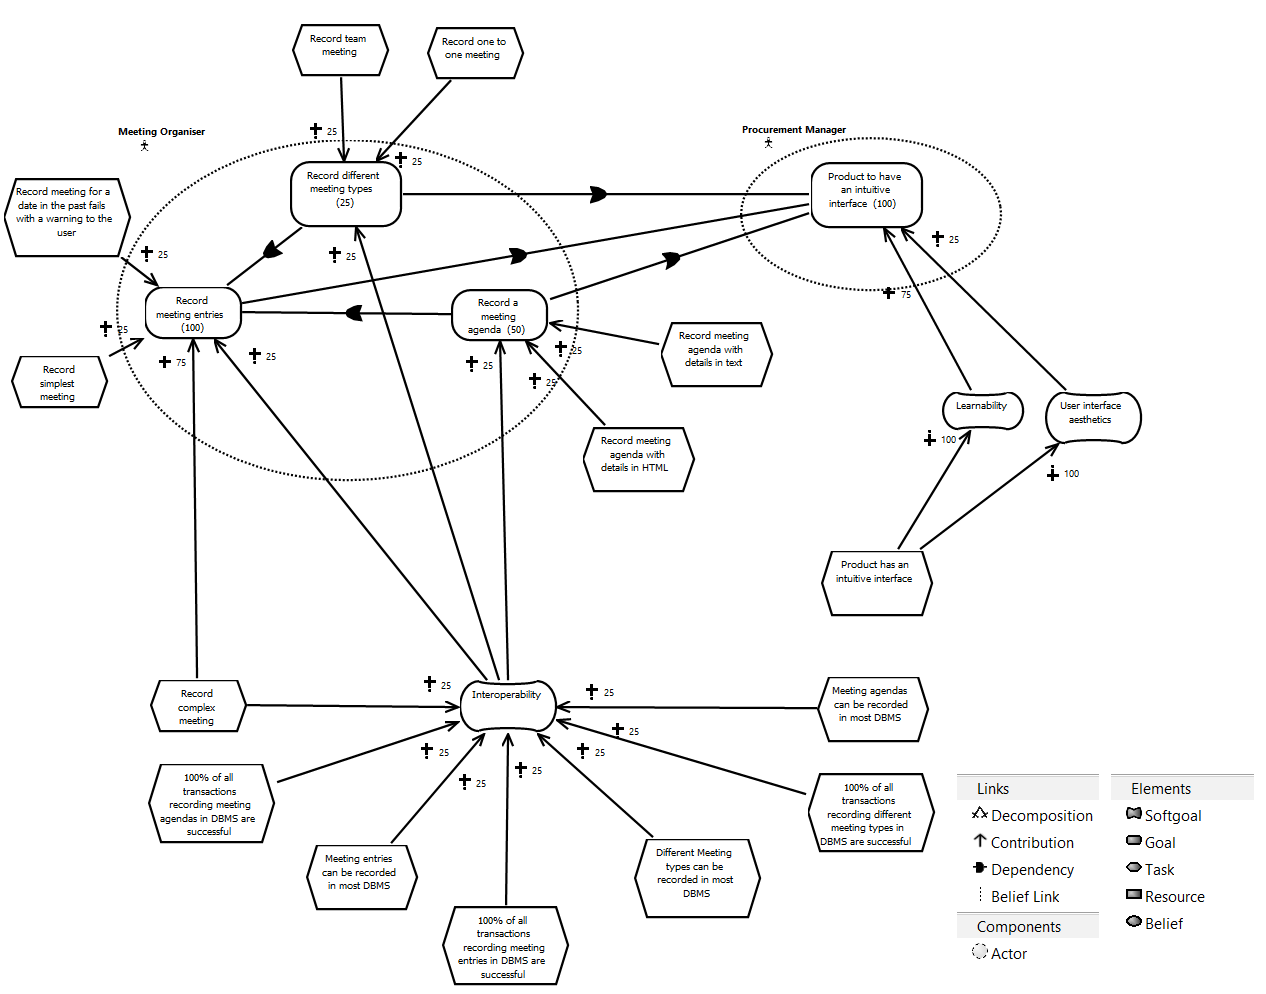
\includegraphics[width=\columnwidth]{casestudy-initial}
\centering
\caption{Case study GRL Graph -- Initial}
\label{fig:InitialGRLGraph}
\end{sidewaysfigure}

The model shows two actors (modelled as circles drawn with dashed lines), and within each, their set of goals defined in the story format extension for feature files described earlier. We can also observe dependencies (thick lines with a filled arrow in the middle) pointing from a dependent goal to others it depends upon (e.g. \emph{Record a meeting agenda} depends upon \emph{Record meeting entries}). 

Also, all global qualities have incoming dependencies from all other goals (e.g. refer to \emph{Product to have an intuitive interface} in the model).

Three \emph{Softgoals} are shown, namely \emph{Interoperability}, \emph{Learnability} and \emph{User interface aesthetics} that also correspond to the ones identified earlier. Note that these \emph{Softgoals} have to be previously defined, and our translator will ensure these are present by including a set of quality softgoals and decompositions with each run of the translator. We have chosen to base this set in the quality characteristics defined in~\citet{ieee_std_25010} but it could be tailored to different categorisation schemes. This process will be described in more detail in chapter~\ref{ch:gherkin_redux}.

The hexagons define \emph{Tasks} in GRL corresponding to scenarios defined in the feature files, with some contributing to Goals,  other to Softgoals, and others to both (e.g. \emph{Record complex meeting} contributes to \emph{Interoperability} softgoal and to \emph{Record meeting entries} goal).

The \emph{contribution} lines (thick lines with arrows at the end) show a symbol and also a numeric value to depict the intended contribution level). These correspond to the contribution levels described in chapter~\ref{ch:nfr_research}, section~\ref{sec:gore}.

Using GRL and the jUCMNav tool, we are able to develop analysis procedures by evaluating qualitative or quantitative satisfaction levels of the actors and intentional elements (e.g., goals and tasks) composing the model~\citep{Amyot2010}.

\citet{Amyot2010} mentions that the analysis of goal models can be done in very different ways depending on the nature of the model and the purpose of the analysis. We believe that in our methodology, there are at least two types of analysis worth considering. 

The first one consists of taking the model as it currently is, and assign initial satisfaction levels to some of the leaf nodes corresponding to the \emph{Tasks} in the model. This corresponds to scenarios being satisficed (or not) and triggering the satisfaction levels of goals and actors. In early stages of the software life-cycle, we may be interested in modelling the potential impact of scenarios in goal satisfaction of one or more stakeholders. In later stages, perhaps we have those scenarios already implemented and satisfied and want to assess current satisfaction levels of actors, in order to determine how far we may be from delivering software or application that satisfied its stakeholders in a sufficiently manner.

The second analysis type, involves considering design options for \emph{Tasks} and/or \emph{Goals} and then checking the impact of those decisions on the satisfaction levels of goals and actors. The process is very similar to the above, but here we are delving into the design domain and considering alternative options to operationalise -- with the meaning intended by the \emph{NFR Framework} -- goals and tasks.

We will now show instances of these two types of analysis, but before proceeding, we need to specify \emph{importance} levels for each of the goals that are bound to an Actor. For what follows, we set the importance of \emph{Record meeting entries} to \emph{High}, of \emph{Record a meeting agenda} to \emph{Medium} and of \emph{Record different meeting types} to \emph{Low}. The goal \emph{Product to have an intuitive interface} was also set to \emph{High} as it is the only goal for the actor \emph{Procurement Manager}, and that seemed like a logical thing to do. This assignment of importance levels to goals bound to actors, is enforced by jUCMNav, without which we would not be able to assess the satisfaction level of actors in the model.
 
We will start by first considering using the model as it currently is. Initial satisfaction levels for some of the intentional elements are provided in a \emph{strategy} and then propagated to the other intentional elements of the model through the various links that connect them. We start by satisfying all \emph{Tasks} corresponding to `functional' scenarios (see figure~\ref{fig:casestudy-functionalscenarios}), that is, those that are not tagged with \emph{NFR}.

\begin{sidewaysfigure}
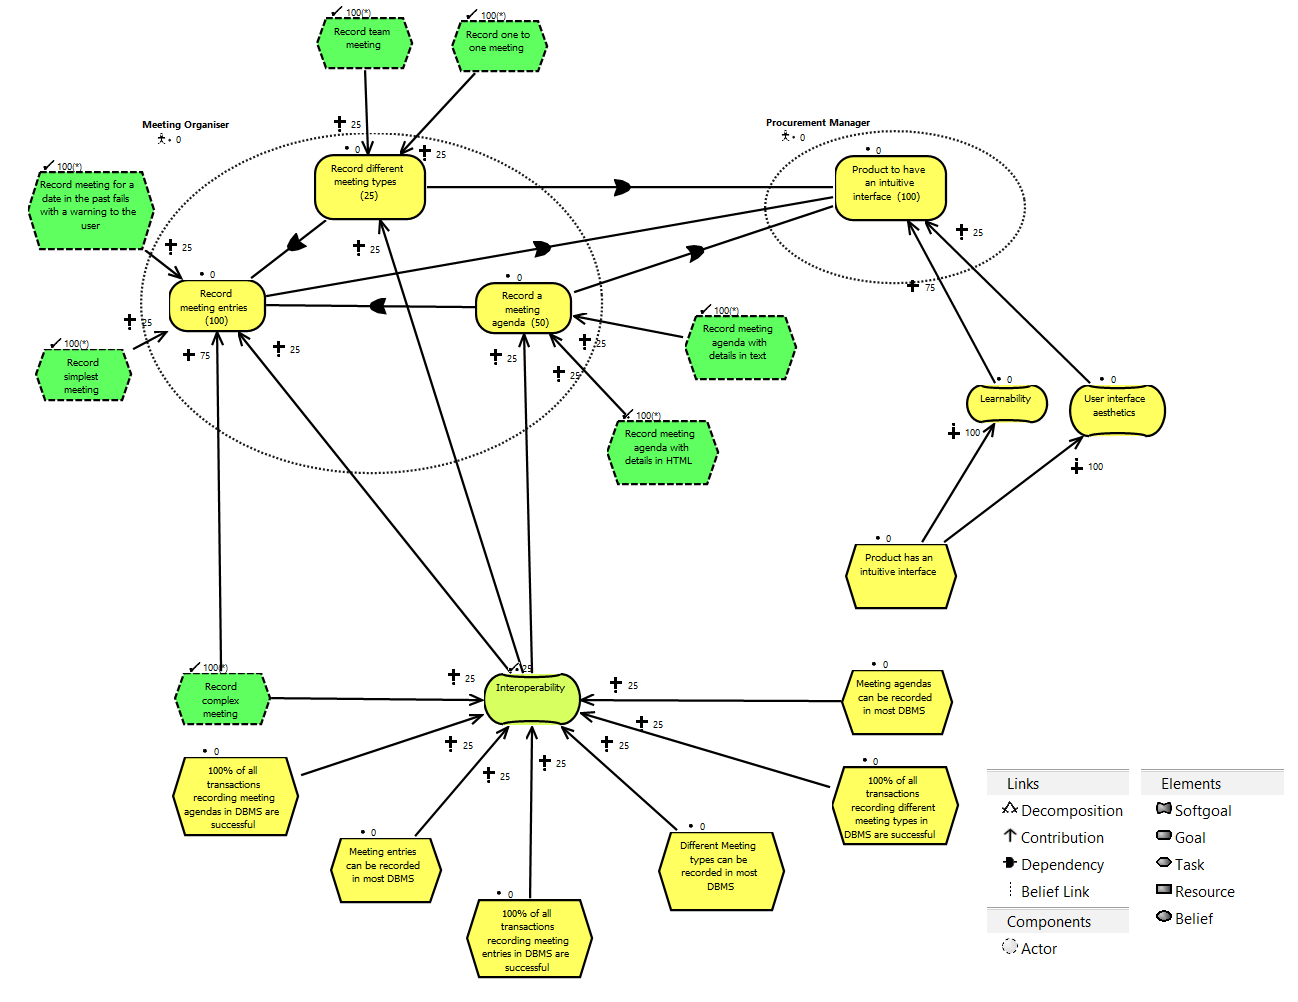
\includegraphics[width=\columnwidth]{casestudy-functionalscenarios}
\centering
\caption{Case study GRL Graph -- All functional scenarios satisfied}
\label{fig:casestudy-functionalscenarios}
\end{sidewaysfigure}

We can note that both goals and actors have their satisfaction level untouched (showing zero on top of the respective icon). This is consistent with our expectation, since all goals are dependent on the \emph{Product to have an intuitive interface} which we haven't yet specified a satisfaction level, and the current strategy did not cause a change to its satisfaction level. It is interesting to note the impact on both goals and actors of setting the satisfaction of that global constraint to either \emph{Satisfied} (see figure~\ref{fig:casestudy-functionalscenarios-globalconstraint}) or \emph{Weakly Denied} (see figure~\ref{fig:casestudy-functionalscenarios-globalconstraint-denied}). The latter satisfaction level, could be interpreted, for example, as an indication of some users being dissatisfied with the user interface or the team facing some implementation issues with some of the application's screens.

\begin{sidewaysfigure}
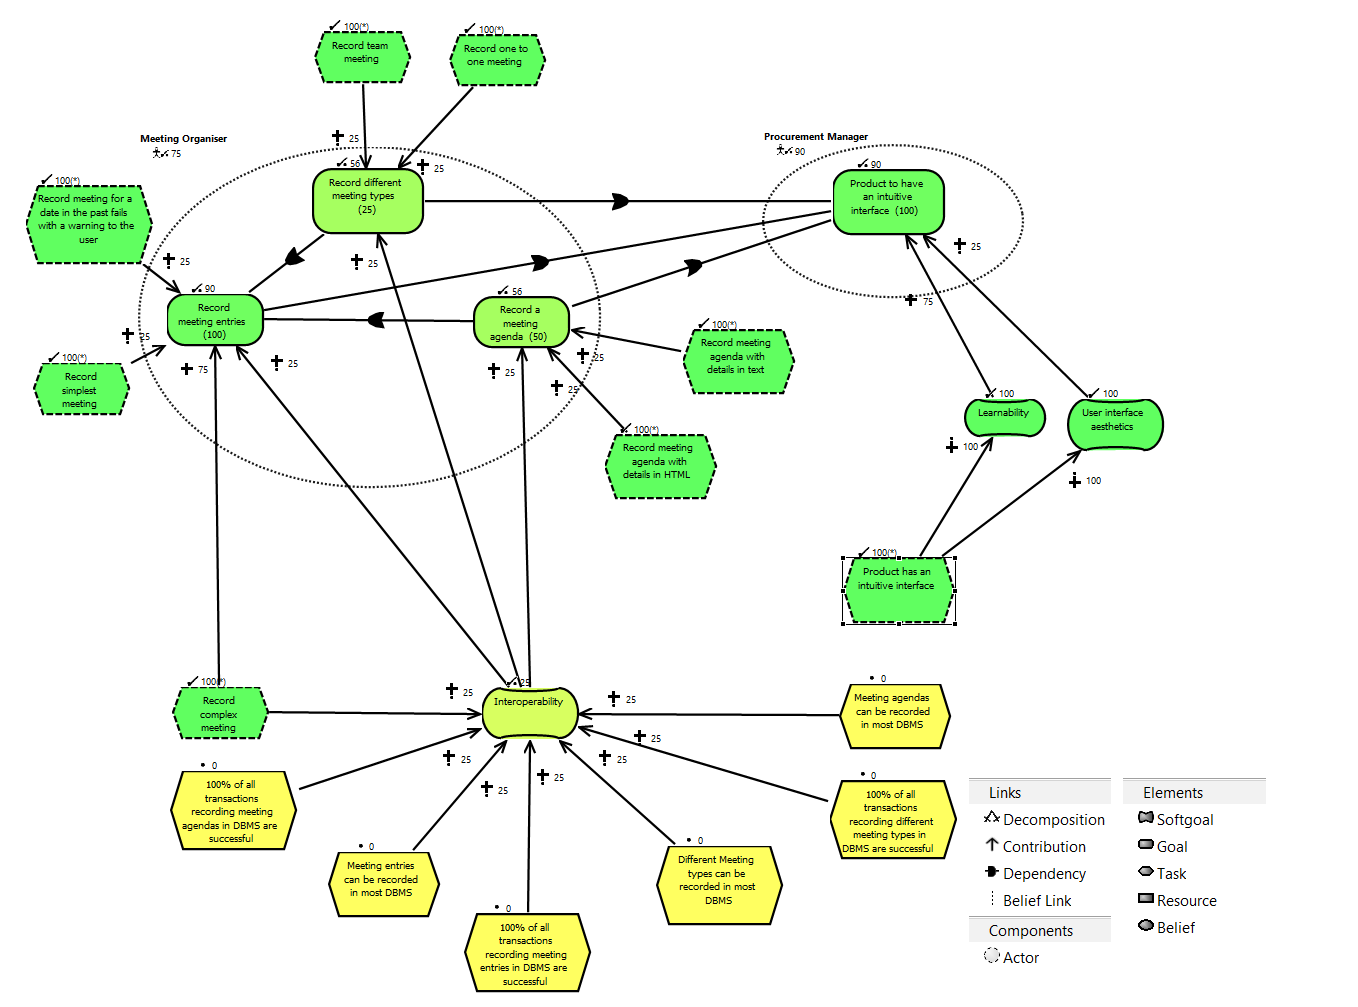
\includegraphics[width=\columnwidth]{casestudy-functionalscenarios-globalconstraint}
\centering
\caption{Case study GRL Graph -- All functional scenarios and global constraint satisfied}
\label{fig:casestudy-functionalscenarios-globalconstraint}
\end{sidewaysfigure} 

\begin{sidewaysfigure}
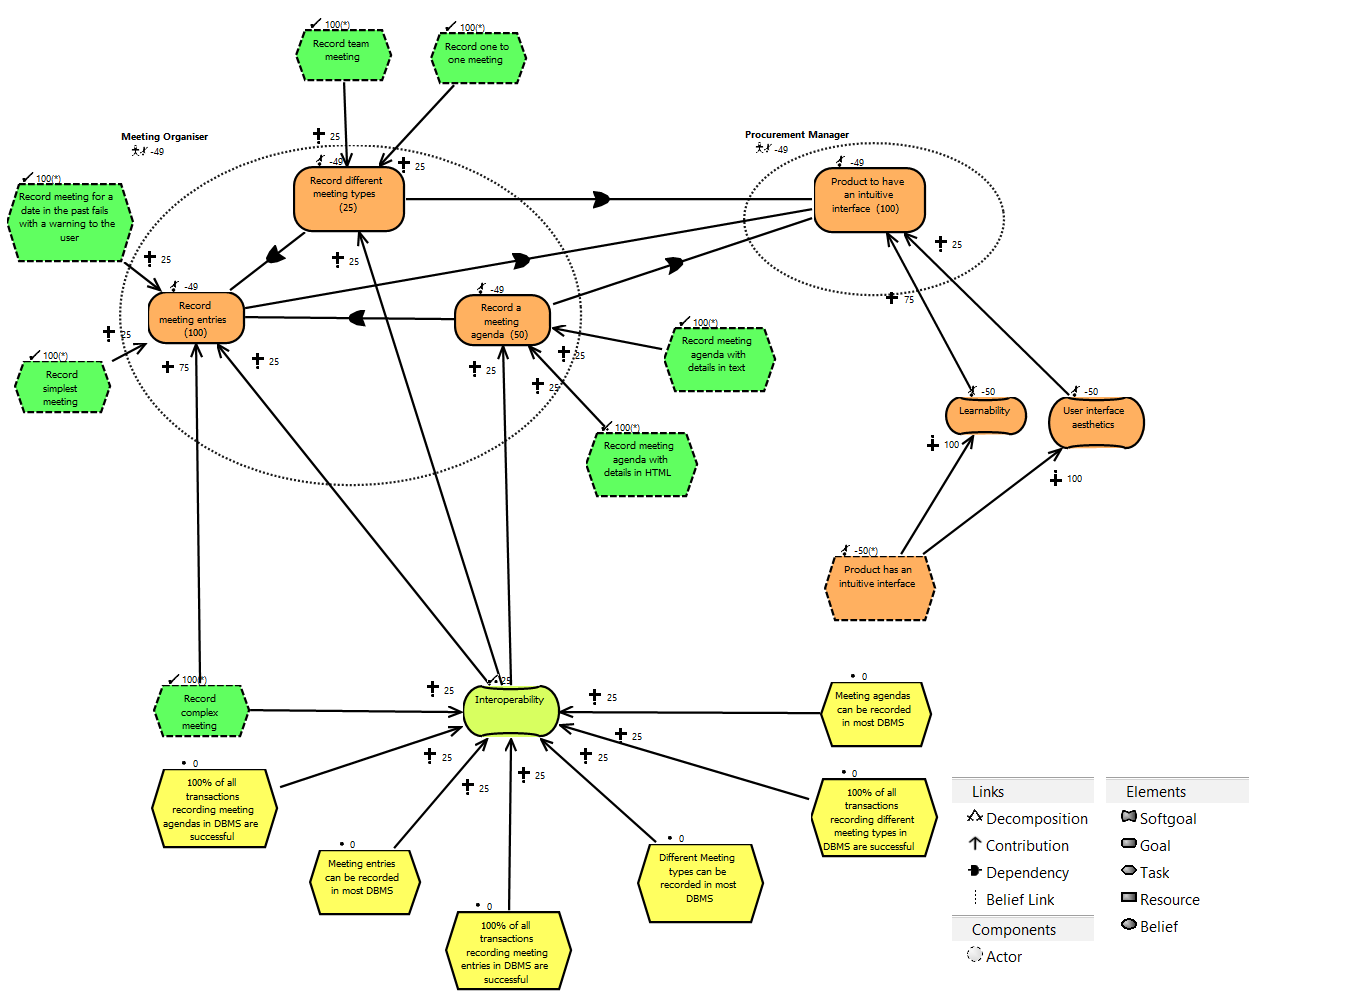
\includegraphics[width=\columnwidth]{casestudy-functionalscenarios-globalconstraint-denied}
\centering
\caption{Case study GRL Graph -- All functional scenarios satisfied, global constraint weakly denied}
\label{fig:casestudy-functionalscenarios-globalconstraint-denied}
\end{sidewaysfigure} 

What can be confirmed from the model is the importance that quality \emph{Product to have an intuitive interface} has on the satisfaction level of goals and actors. When it is weakly denied the satisfaction level of other goals and actors is constrained to the minimum of their own satisfaction levels and the one of the global quality (e.g. -49 in this case). This should be a sign that the agile team should dedicate more attention and resources to improve attainability of that quality (this could be achieved by fixing any issues found or investing time in improving current implementation).

We can also consider design alternatives and perform an assessment of the relative effectiveness of these alternatives at the requirements level~\citep{Amyot2010}. Figure~\ref{fig:casestudy-designoptionsA} shows the same model as before but where some design options have been considered. In particular, \emph{High availability} has been considered as a design option to help ensure $100\%$ of all transactions in DBMS~\footnote{~Database Management Systems (DBMS)} are successfull; one of \emph{Use ORM}~\footnote{~Object Relational Mapping} or \emph{Use standard T-SQL only} were considered as options to attain interoperability with most DBMS and two distinct options were considered to address the constrain specified that the product should have an intuitive interface. The particular strategy chosen is a valid one as it ensures all goals and actors attain a positive satisfaction level. It may not be adequate if say, for example, there are other strategies that provide a better satisfaction level for the \emph{Meeting Organiser} and this has been considered a key stakeholder.

Figure~\ref{fig:casestudy-designoptionsB} shows the same model as before, with the same design options considered but with a different strategy. Here, by using an \emph{external UI library} the satisfaction level of goals and actors is improved, even though \emph{Interoperability} as a quality is \emph{Weakly Denied}. This may be an acceptable strategy, if we are trying to maximise satisfaction levels of actors and goals and attaining \emph{Interoperability} is not as important.

\begin{sidewaysfigure}
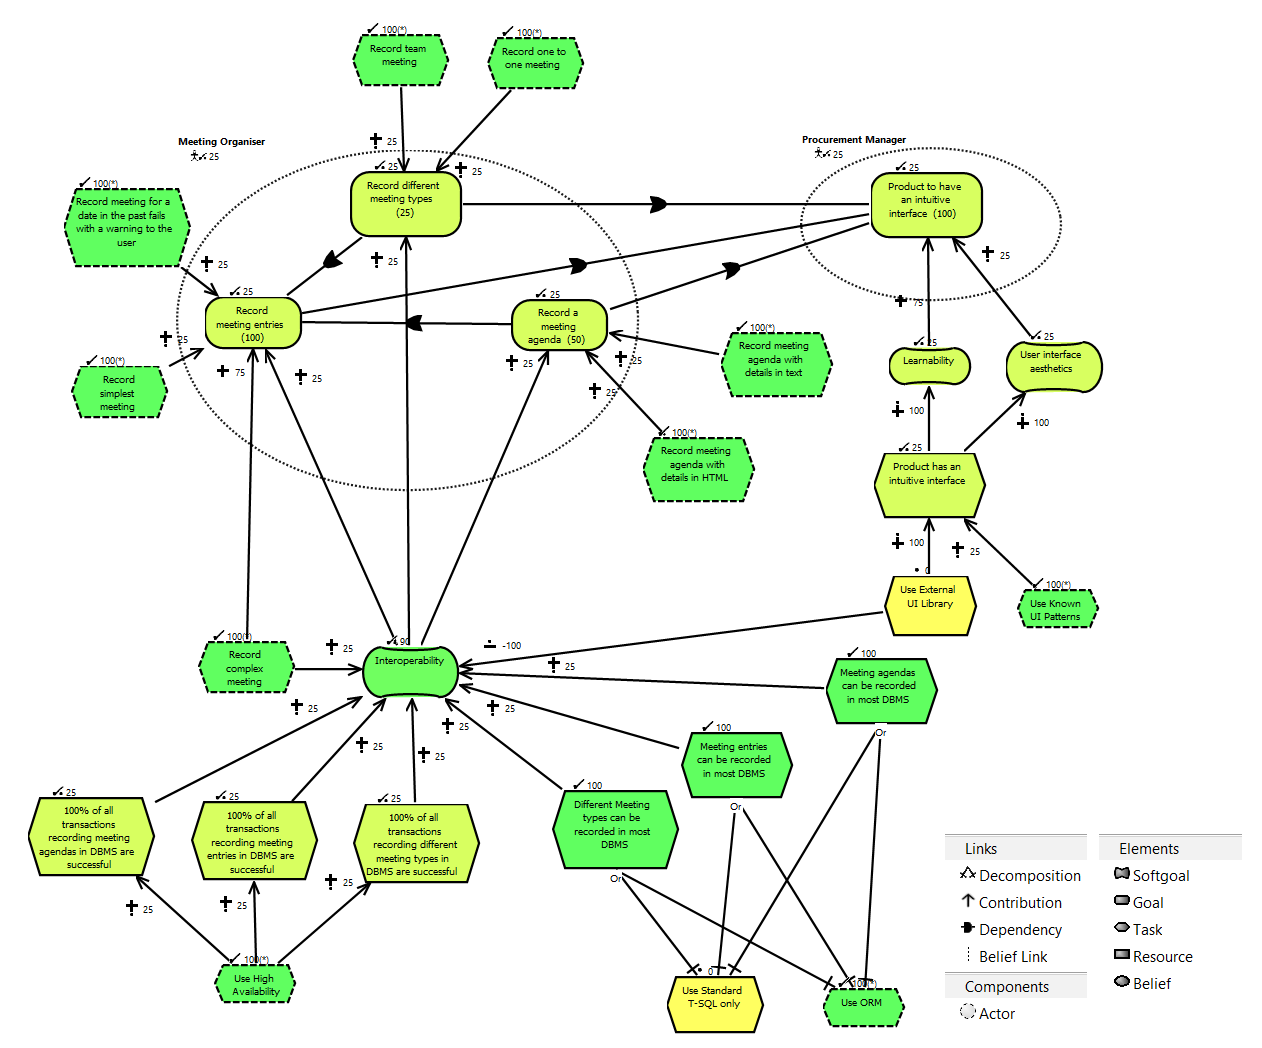
\includegraphics[width=\columnwidth]{casestudy-designoptionsA}
\centering
\caption{Case study GRL Graph -- Design options considered (Option A)}
\label{fig:casestudy-designoptionsA}
\end{sidewaysfigure}

\begin{sidewaysfigure}
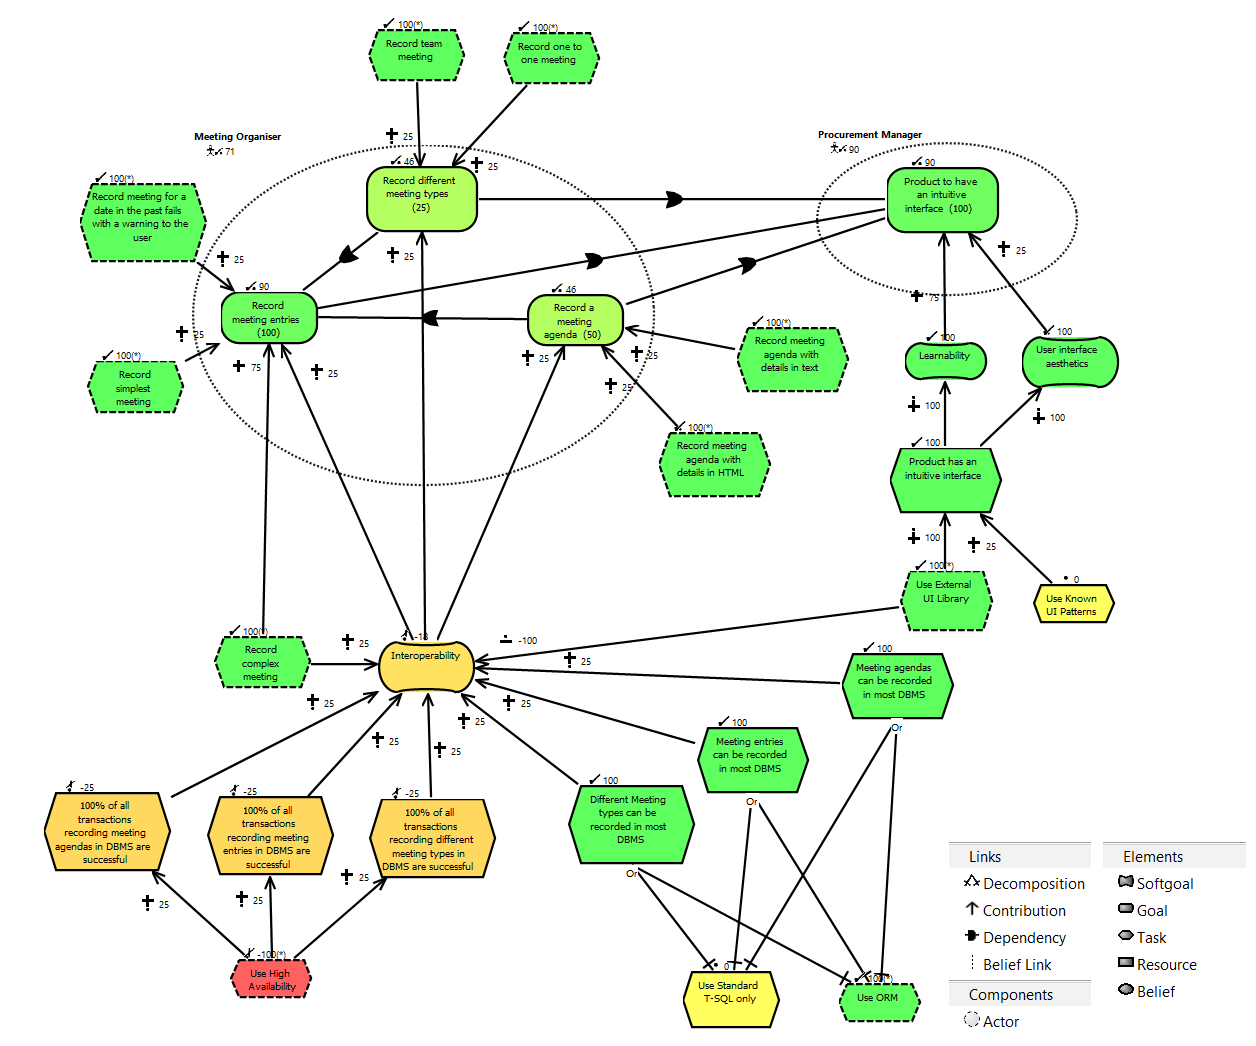
\includegraphics[width=\columnwidth]{casestudy-designoptionsB}
\centering
\caption{Case study GRL Graph -- Design options considered (Option B)}
\label{fig:casestudy-designoptionsB}
\end{sidewaysfigure}

\section{Summary}
In this chapter, and in the context of Behaviour-driven development, we have described a methodology that addresses \nfrs in tandem with functional requirements. We have done it, by introducing a goal-oriented approach to the elicitation, analysis and modelling of requirements as aspirational goals of one or more identified stakeholders of an application or system.

We initially described, through a series of small transformational steps, the set of required changes to Gherkin, in order to translate requirements into goals, determine any dependencies and conflicts between goals, and more importantly, evaluate satisfaction levels of goals and actors.

We have made use of a well known public dataset and, sampled a subset of functional and non-functional requirements to support the description of our methodology. In doing so, we have showed how requirements specified in Gherkin can be transformed into a GRL catalogue of intentional elements and modelled as a GRL graph in a specialised tool such as jUCMNav.

In the next chapter we will describe in detail the implementation changes to the Gherkin parser and also a tool to convert one or more feature files into a GRL catalogue suitable to be imported and further refined and analysed into jUCMNav.

\chapter{From Gherkin to GRL}
\label{ch:gherkin_redux}

It is important to note that Gherkin has been localised for several languages. In our research, we only extended the English language keywords, but it would be relatively easy to add support for more languages. Gherkin uses \emph{Json}~(Javascript Object Notation)~\footnote{see http://json.org/ for details} -- a lightweight data-interchange format -- to represent keywords in all supported languages. Listing below shows the English keywords supported, including the ones we added in this work, that is \emph{asA}, \emph{iWant}, \emph{soThat}, \emph{qualityAttribute}, \emph{qualityReason}, \emph{scenarioContribution} and \emph{whichMayImpact}.

\begin{featurelist}{Extended Gherkin -- English keywords}{lst:gherkin_keywords}
\begin{featurecode}{0.7}
\begin{minted}{json}
{
"en": {
        "and": [
            "* ",
            "And "
        ],
        "background": [
            "Background"
        ],
        "but": [
            "* ",
            "But "
        ],
        "examples": [
            "Examples",
            "Scenarios"
        ],
        "feature": [
            "Feature",
            "Business Need",
            "Ability"
        ],
        "given": [
            "* ",
            "Given "
        ],
        "name": "English",
        "native": "English",
        "scenario": [
            "Scenario"
        ],
        "scenarioOutline": [
            "Scenario Outline",
            "Scenario Template"
        ],
        "then": [
            "* ",
            "Then "
        ],
        "when": [
            "* ",
            "When "
        ],
        "asA": [ "As a " ],
        "iWant": [ "I want to ", "I want the" ],
        "soThat": [ "So that " ],
        "qualityAttribute": [ "Without ignoring" , "Constrained by"],
        "qualityReason": [ "By " ],
        "scenarioContribution": [
            "Breaking the ",
            "Which breaks ",
            "Contributing to break ",
            "Helping the ",
            "Which helps ",
            "Contributing to help ",
            "Hurting the ",
            "Which hurts ",
            "Contributing to hurt ",
            "Making the ",
            "Which makes ",
            "Contributing to make ",
            "With some positive contribution to ",
            "With some negative contribution to "
        ],
        "whichMayImpact": [ "Which may impact " ]
    },
}
\end{minted}
\end{featurecode}
\end{featurelist}

\begin{figure}[h!]
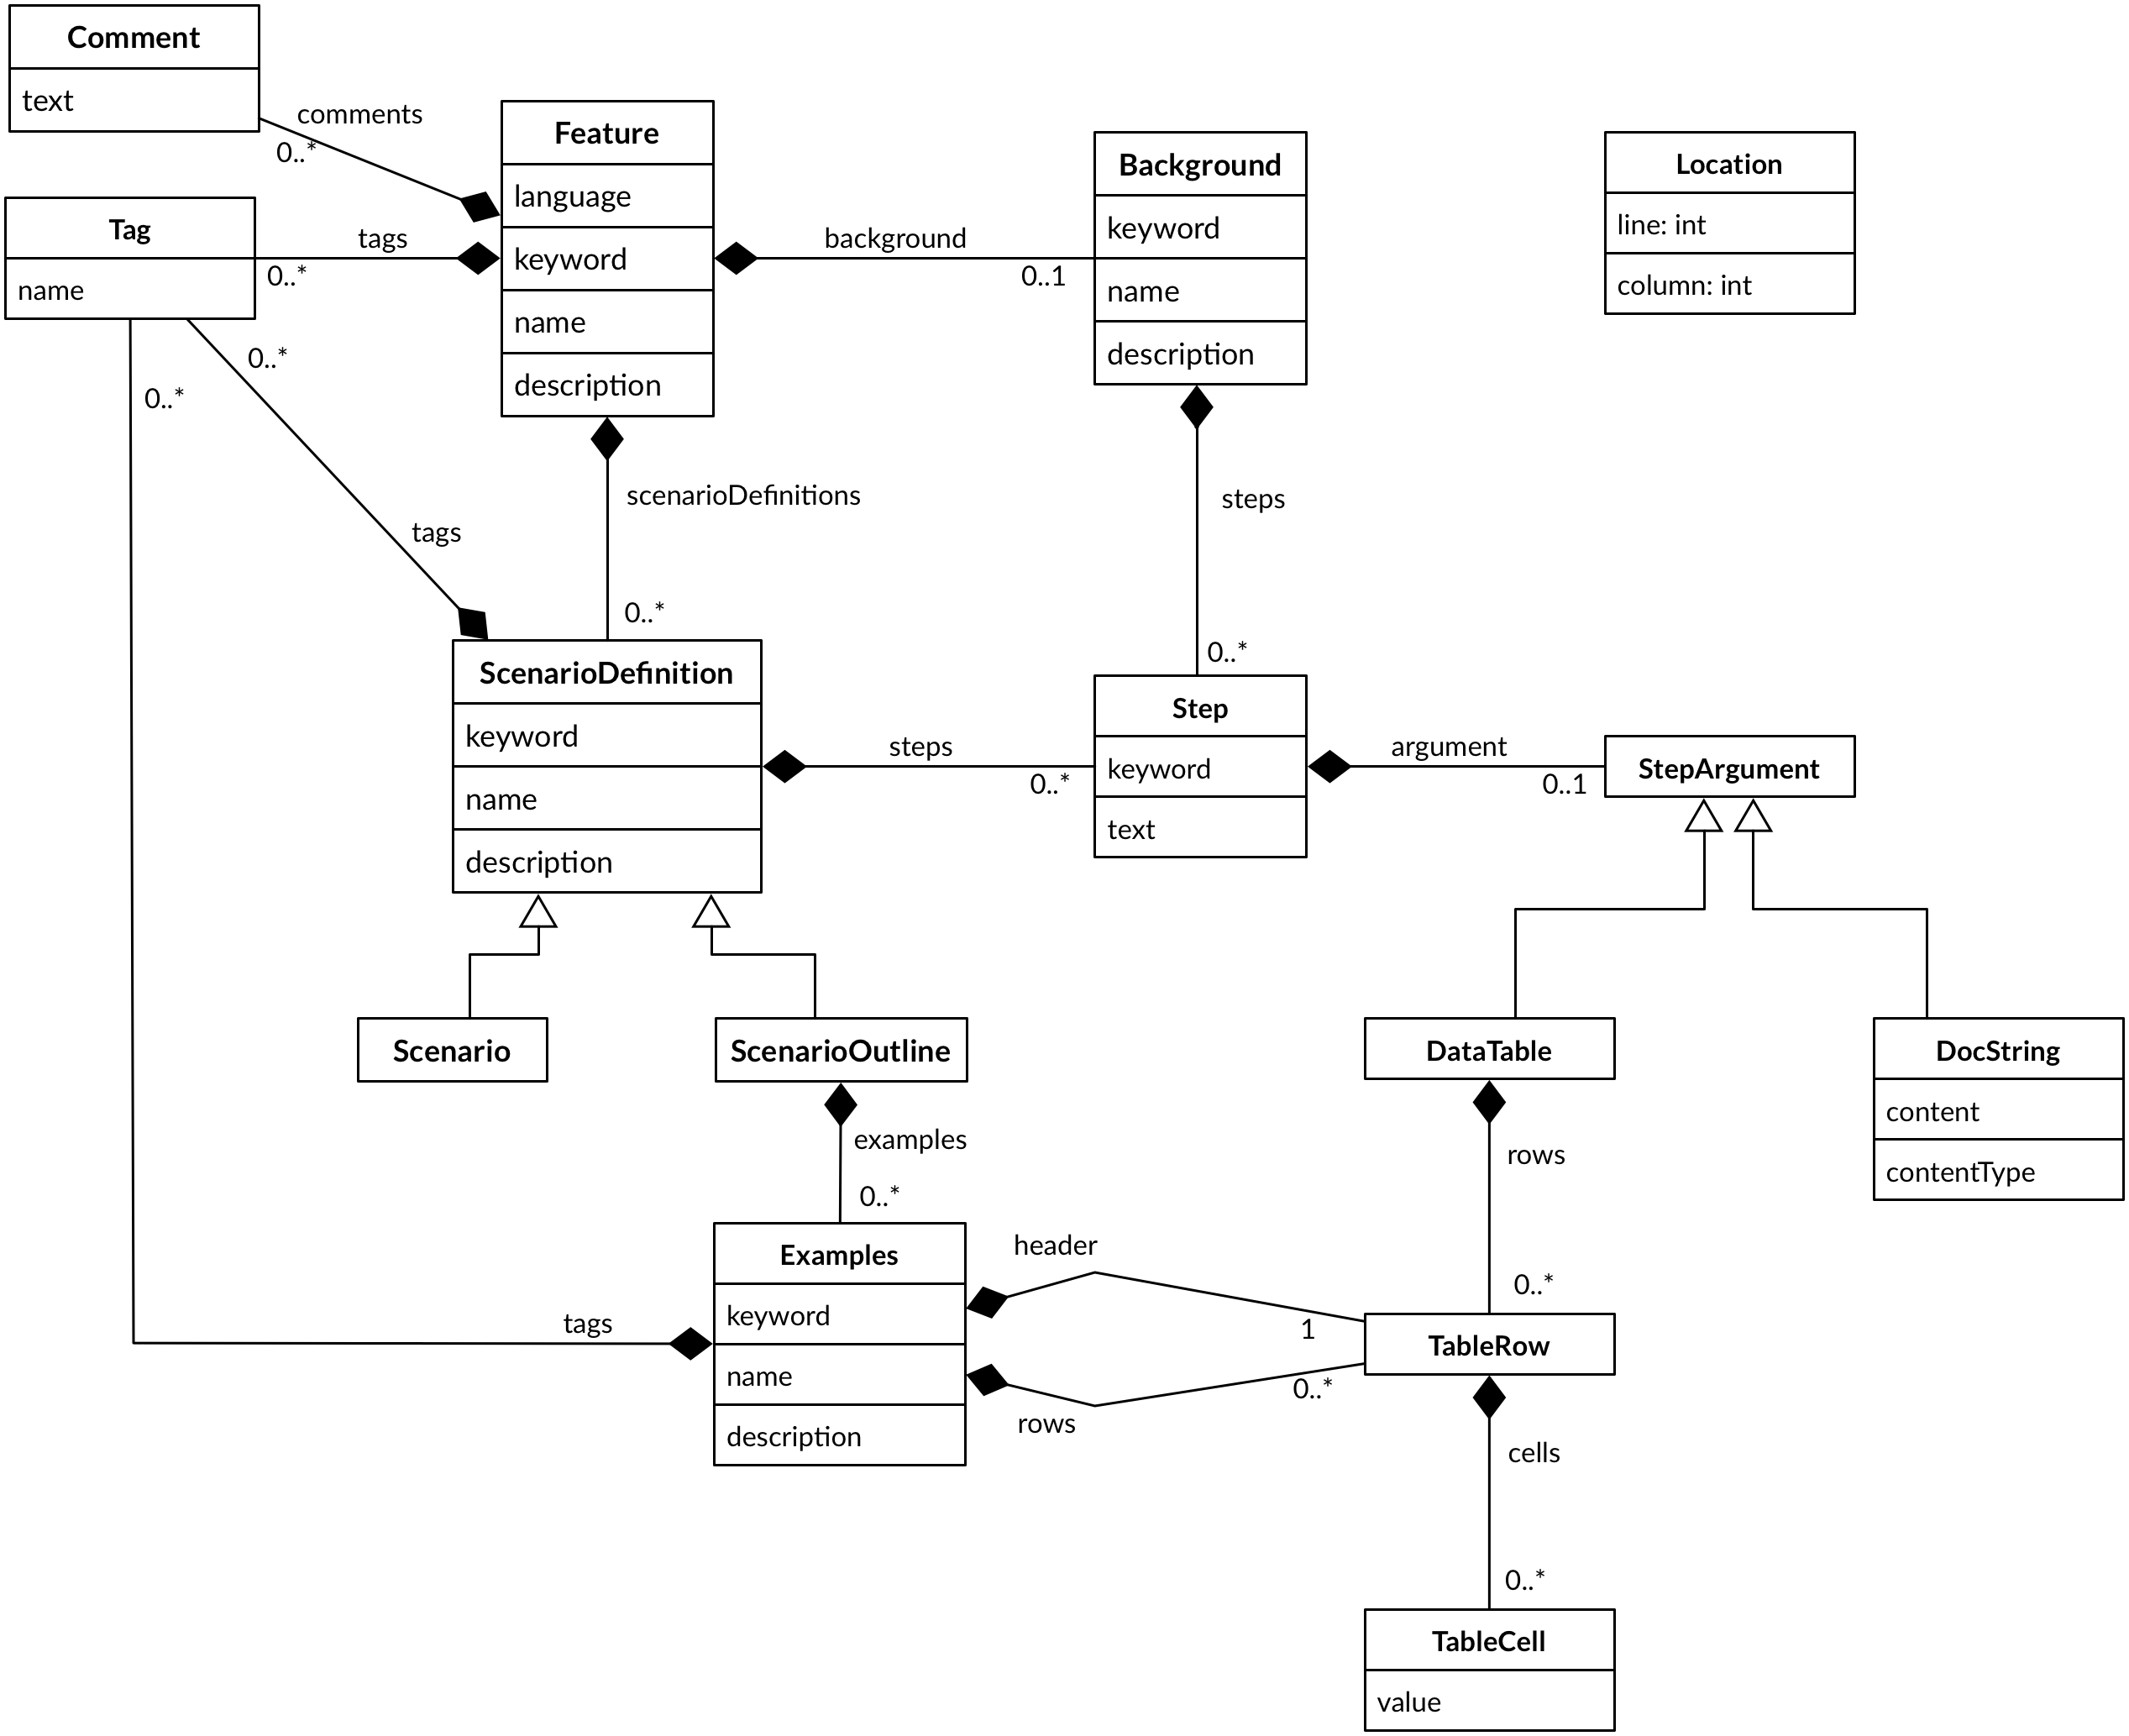
\includegraphics[width=0.85\textwidth]{gherkin3_ast}
\centering
\caption[Original Gherkin class model]{Original Gherkin class model~\footnotemark}
\label{fig:gherkin_ast}
\end{figure}
\footnotetext{~extracted from the Gherkin wiki at https://github.com/cucumber/gherkin3}

\chapter{Conclusion}
\label{ch:Conclusion}
Most conventional approaches to system design are driven by functional requirements. Developers focus their efforts primarily on achieving the desired functionality of a product or system, usually considering non-functional requirements (such as cost and performance) in a non-systematic and often undocumented way~\citep{Chung2000}. Furthermore, these software quality attributes are often addressed late and viewed as consequences of the decisions rather than as goals to be achieved.

Out work helps to address some of the most common requirements risks~\citep[p. 20]{Wiegers2013}.
\begin{itemize}
\item Insufficient user involvement
\item Inaccurate planning
\item Creeping user requirements
\item Ambiguous requirements
\item Gold plating
\item Overlooked stakeholders
\end{itemize}
\appendix
Our work is also actual and contributes to major requirements trends in recent in the past decade, including
\begin{itemize}
\item The recognition of business analysis as a professional discipline
\item The maturing of tools both for managing requirements in a database and for assisting with requirements development activities such as prototyping, modelling, and simulation
\item The increased use of agile development methods and the evolution of techniques for handling requirements on agile projects
\item The increased use of visual models to represent requirements knowledge
\end{itemize}

Writing the requirements isn't the hard part. The hard part is determining the requirements. Writing requirements is a matter of clarifying, elaborating, and recording what you've learned. A solid understanding of a product's requirements ensures that your team works on the right problem and devises the best solution to that problem. Without knowing the requirements, you can't tell when the project is done, determine whether it has met its goals, or make trade-off decisions when scope adjustments are necessary. It can cost far more to correct a defect that's found late in the project than to fix it shortly after its creation. Shortcomings in requirements practices pose many risks to project success, where success means delivering a product that satisfies the user's functional and quality expectations at the agreed-upon cost and schedule~\citep{Wiegers2013}.

Some of the most common requirements risks are insufficient user involvement; inaccurate planning; creeping user requirements ; ambiguous requirements and overlooked stakeholders. Sound requirements processes emphasize a collaborative approach to product development that involves stakeholders in a partnership throughout the project. Eliciting requirements lets the development team better understand its user community or market, a critical success factor. Emphasizing user tasks instead of superficially attractive features helps the team avoid writing code that no one will ever execute. Customer involvement reduces the expectation gap between what the customer really needs and what the developer delivers. Documented and clear requirements greatly facilitate system testing. All of these increase your chances of delivering high-quality products that satisfy all stakeholders~\citep{Wiegers2013}.

A central point for the distinction of functionality and other qualities is that, for software construction, the purpose of the software system needs to be well defined in terms of the functions that the software will perform~\citep{Chung:2009vg}.

The distinction between functionality and other qualities in the field of requirements engineering has an important benefit: it makes clear to software engineers that requirements are meant to deal with quality attributes and not with just one of them. As the software industry became more mature and different domains were explored by software engineers, it became clearer that it would not be enough just to deal with the description of the desired functionality, but that quality attributes should be carefully thought of early on as well~\citep{Chung:2009vg}.

Not only non-functional requirements need to be stated up front, but they can help the software engineer make design decisions, while also justifying such decisions. However, in order to take this into consideration, it is necessary that quality attributes not be considered just as a separate set of requirements, but with the consideration of the functionality throughout the development process~\citep{Chung:2009vg}.

\fxnote{Describe the role tools (e.g. Cucumber) could play in marking scenarios as passed and in GRL the corresponding tasks marked as satisficed}

\fxnote{Our changes to Gherkin did not introduce any GRL specific concept. Separation of concerns}

\chapter{Typical chapter contents}\fxnote{Remove}


\underline{Start of chapter}
\paragraph{General advice}
Link back to previous parts in particular previous chapter\\
State the aim of the chapter\\
Outline how you intend to achieve this aim in the form of an overview of contents\\

\noindent\underline{Contents}
\paragraph{Discussion or Analysis}
\begin{itemize}
\item What's important
\item What overall themes can be identified
\item What can be observed or learned
\item What limitations or shortcomings have been identified
\item Situate the chapter within the whole thesis
\end{itemize}
\paragraph{Summary}
\begin{itemize}
\item Replies to the introduction by briefly identifying the chapter's achievements and sets the scene for the next chapter
\end{itemize}

\noindent\underline{End of chapter}
\paragraph{General advice}
Start with a strong summary of the main findings of this chapter with academic references and relate it with current theory.\\
Relates this chapter results to earlier analysis.\\
End with a strong lead into next chapter.\\

\begin{appendices}
\chapter{Case Study}
\label{ch:case_study_appendix}
The table below lists all the original non-functional requirements for the \emph{meeting scheduler} project included in  the \emph{PROMISE} dataset, including the classification proposed by \citeauthor{MylopoulosOnt2014} in \cite{MylopoulosOnt2014}. Note that for easy of referencing the table retains original requirement identifiers.

\ifdraft{%
  \fxnote{THIS WILL CONTAIN NFRS TABLE}
}{%

\begin{center}
\begin{longtable}{c c m{.6\textwidth}}
\caption[Meeting scheduler original non-functional requirements]{Meeting scheduler original non-functional requirements~(\emph{PROMISE}, 2015)\label{tb:scheduler_original_nfrs}}\\
\toprule \multicolumn{1}{c}{\bfseries{Requirement ID}} & \multicolumn{1}{c}{\bfseries{Classification}} & \multicolumn{1}{c}{\bfseries{Non-functional Requirement Description}}\\
    \addlinespace
    \midrule
    \endfirsthead
\multicolumn{3}{c}%
{\tablename\ \thetable\ -- \textit{Continued from previous page}} \\
\toprule \multicolumn{1}{c}{\bfseries{Requirement ID}} & \multicolumn{1}{c}{\bfseries{Classification}} & \multicolumn{1}{c}{\bfseries{Non-functional Requirement Description}}\\
    \addlinespace
    \midrule
\endhead
\multicolumn{3}{r}{\textit{Continued on next page}} \\
\endfoot
\addlinespace
\bottomrule
\endlastfoot
    R 138   & FR+QR & The product must work with most database management systems (DBMS) on the market whether the DBMS is colocated with the product on the same machine or is located on a different machine on the computer network. \\
    \midrule
    R 139   & FR+QR & The product will function alongside server software on any operating system where the Java runtime can be installed. \\    \midrule
    R 140   & FR & The product will require collaboration with a database management system (DBMS). The DBMS may be located on the same machine as the product or on a separate machine residing on the same computer network. \\    \midrule
    R 141   & QR & The product must make use of web/application server technology. Open source examples include Apache web server Tomcat and the JBoss application server. \\    \midrule
    R 142   & FR & A database management system such as Oracle DB2 MySql or HSQL will need to be integrated with the product \\    \midrule
    R 143   & FR+QR & The product's Look and Feel shall be able to incorporate aspects of the customer's organization such as logo branding and identity \\    \midrule
    R 144   & QR & The product shall have a conservative and professional appearance \\    \midrule
    R 145   & QR & The product shall make the users want to use it. 80\textbackslash{}\% of the users surveyed report they are regularly using the product after the first 2 weeks postlaunch \\    \midrule
    R 146   & QR & The product shall be easy to use. 90\textbackslash{}\% of users will be able to successfully reserve a conference room within 5 minutes of product use \\*    \midrule
    R 147   & FR+QR & The product shall give users feedback when necessary. 80\textbackslash{}\% of the users surveyed report that the product accurately confirms their actions \\    \midrule
    R 148   & FR+QR & The product shall allow the user to select a chosen language from one of the target market countries \\ \midrule
    R 149   & FR+QR & The product shall allow for customization of start page and views preferences \\    \midrule
    R 150   & QR & An employee will be able to successfully use the product within a few minutes. After informally navigating the product for less than 15 minutes users shall be able to successfully setup meetings and reserve conference rooms \\    \midrule
    R 151   & QR & The product shall use a standard navigation menu familiar to most web users \\    \midrule
    R 152   & FR+QR & The product shall allow for intuitive searching of available conference rooms \\    \midrule
    R 153   & QR & The product shall conform to the Americans with Disabilities Act \\    \midrule
    R 154   & QR & The response shall be fast enough to avoid interrupting the user's flow of thought. 90\textbackslash{}\% of tasks shall complete within 5 seconds. 98\textbackslash{}\% of tasks shall complete within 8 seconds \\    \midrule
    R 155   & QR & Aside from server failure the software product shall achieve 99.99\textbackslash{}\% up time \\    \midrule
    R 156   & FR+QR &  The product shall create an exception log of problems encountered within the product for transmission to our company for analysis and resolution \\    \midrule
    R 157   & QR & The product shall be capable of handling up to 1 000 concurrent requests. This number will increase to 2 000 by Release 2. The concurrency capacity must be able to handle peak scheduling times such as early morning and late afternoon hours \\    \midrule
    R 158   & QR & The product shall be able to process 10 000 transactions per hour within two years of its launch. This number will increase to 20 000 by Release 2 \\    \midrule
    R 159   & QR & The product shall be expected to operate for at least 5 years for each customer installation \\    \midrule
    R 160   & DA & The product shall be used in office environments \\    \midrule
    R 161   & FR+QR & The product must be able to interface with any HTML browser. The product shall transmit data between the user and the product without problems. The product shall display HTML properly in 80\textbackslash{}\% of all HTML browsers tested (minimum is to test 8 browsers) \\    \midrule
    R 162   & FR+QR & The product must be able to interface with various database management systems. The product shall communicate successfully with the database management system on 100\textbackslash{}\% of all transactions. \\    \midrule
    R 163   & FR+QR & The product must be able to interface with various email servers. The product shall be able to send email \\    \midrule
    R 164   & FR & The product shall be available for distribution via the Internet as a binary or ZIP file \\    \midrule
    R 165   & FR & The product shall be available for distribution as a packaged CD \\    \midrule
    R 166   & FR & The product will be available for licensing as a one-server two-five servers or five-or-more servers license \\    \midrule
    R 167   & QR & A new user must be able to be added to the system within 10 minutes.90\textbackslash{}\% of new users are able to log into the system within 10 minutes \\    \midrule
    R 168   & QR & The product must be designed using Design Patterns and coding best practices. 90\textbackslash{}\% of maintenance software developers are able to integrate new functionality into the product with 2 working days \\    \midrule
    R 169   & QR & The product must be highly configurable for use with various database management systems for the end users. 80\textbackslash{}\% of end users are able to integrate new database management systems with the product without changing the product's software code \\    \midrule
    R 170   & QR & Maintenance releases will be offered to customers once a year. The releases shall take no longer than 5 minutes for 80\textbackslash{}\% of the customer base to install \\    \midrule
    R 171   & FR+QR & Every registered user will have access to the product's support site via the Internet. 70\textbackslash{}\% of registered users shall find a solution to their problem within 5 minutes of using the support site \\    \midrule
    R 172   & QR & The customer shall be able to easily integrate new building maps with the product throughout the product's life-cycle. Integration of new maps with the product shall be possible with little to no support from product support staff \\    \midrule
    R 173   & FR+QR & The product shall be translated into foreign languages other than the target market countries languages in future releases. For each emerging target market it shall take no more than 5 days to configure the product for that market's language \\    \midrule
    R 174   & FR+QR & The product is expected to integrate with multiple database management systems. The product will operate with Oracle SQL Server DB2 MySQL HSQL and MS Access \\    \midrule
    R 175   & QR & The product shall be able to be installed in any operating environment within 2 days \\    \midrule
    R 176   & CF+QR & The product shall ensure that only company employees or external users with company-approved user IDs may have product access. 100\textbackslash{}\% of all logons shall be by either company employees or external users with company-approved user IDs \\    \midrule
    R 177   & CF+QR & Only managers are able to perform search queries for reservations by user. 100\textbackslash{}\% of all search queries for reservations by user shall be from logons of only management logons \\    \midrule
    R 178   & FR+QR & The product shall ensure that the database's data corresponds to the data entered by the user. Each conference room reservation in the system will contain the same information as was entered by the user \\    \midrule
    R 179   & FR+QR & The product shall prevent the input of malicious data. The product and/or adjacent hardware/software systems data shall remain 100\textbackslash{}\% uncorrupted each time malicious data is input into the product \\    \midrule
    R 180   & QR & The product and/or dependent databases/filesystems shall remain operational as a result of the input of malicious data. The product and/or dependent databases/filesystems shall not crash 100\textbackslash{}\% of the time that malicious data is input into the product \\    \midrule
    R 181   & FR+QR & The product shall have the ability to receive automatic software updates as new threats emerge. 100\textbackslash{}\% of customers will be able to receive automatic software updates transmitted to the installed product \\    \midrule
    R 182   & QR & The language of the product shall accommodate all of the target market countries. 90\textbackslash{}\% of survey respondents from each target market country will find that the language of the product is acceptable \\    \midrule
    R 183   & FR+QR & The product shall be able to display calendar dates and times according to the user's locale. 90\textbackslash{}\% of survey respondents from each target market country will find that the date and time formatting of the product is correct \\    \midrule
    R 184   & QR & The product must be developed with the J2SE/J2EE programming language libraries \\
\end{longtable}
\end{center}
}

\section{Case study requirements in BDD format}

In this section, we list the remaining feature files corresponding to the functional requirements in the \emph{meeting scheduler} case study and not addressed previously in chapter~\ref{ch:Extendingbdd}, section~\ref{sec:case_study}.

\begin{featurelist}{R53 -- The product shall store new conference rooms}{lst:feature_r53}
\begin{featurecode}{0.7}
\inputminted{Gherkin}{D:/Dev/thesis/gherkin3/testdata/extendedBDD/R53.feature}
\end{featurecode}
\end{featurelist}
\clearpage

\begin{featurelist}{R54 -- The product shall record meeting entries}{lst:feature_r54}
\begin{featurecode}{0.7}
\inputminted{Gherkin}{D:/Dev/thesis/gherkin3/testdata/extendedBDD/R54.feature}
\end{featurecode}
\end{featurelist}
\clearpage

\begin{featurelist}{R55 -- The product will be able to delete conference rooms}{lst:feature_r55}
\begin{featurecode}{0.7}
\inputminted{Gherkin}{D:/Dev/thesis/gherkin3/testdata/extendedBDD/R55.feature}
\end{featurecode}
\end{featurelist}
\clearpage

\begin{featurelist}{R56 -- The product shall be able to store new room equipment}{lst:feature_r56}
\begin{featurecode}{0.7}
\inputminted{Gherkin}{D:/Dev/thesis/gherkin3/testdata/extendedBDD/R56.feature}
\end{featurecode}
\end{featurelist}
\clearpage

\begin{featurelist}{R57 -- The product will update existing room equipment}{lst:feature_r57}
\begin{featurecode}{0.7}
\inputminted{Gherkin}{D:/Dev/thesis/gherkin3/testdata/extendedBDD/R57.feature}
\end{featurecode}
\end{featurelist}
\clearpage

\begin{featurelist}{R58 -- The product shall be able to delete room equipment}{lst:feature_r58}
\begin{featurecode}{0.7}
\inputminted{Gherkin}{D:/Dev/thesis/gherkin3/testdata/extendedBDD/R58.feature}
\end{featurecode}
\end{featurelist}
\clearpage

\begin{featurelist}{R60 -- }{lst:feature_r60}
\begin{featurecode}{0.7}
\inputminted{Gherkin}{D:/Dev/thesis/gherkin3/testdata/extendedBDD/R60.feature}
\end{featurecode}
\end{featurelist}
\clearpage

\begin{featurelist}{R61 -- }{lst:feature_r61}
\begin{featurecode}{0.7}
\inputminted{Gherkin}{D:/Dev/thesis/gherkin3/testdata/extendedBDD/R61.feature}
\end{featurecode}
\end{featurelist}
\clearpage

\begin{featurelist}{R62 -- }{lst:feature_r62}
\begin{featurecode}{0.7}
\inputminted{Gherkin}{D:/Dev/thesis/gherkin3/testdata/extendedBDD/R62.feature}
\end{featurecode}
\end{featurelist}
\clearpage

\begin{featurelist}{R64 -- }{lst:feature_r64}
\begin{featurecode}{0.7}
\inputminted{Gherkin}{D:/Dev/thesis/gherkin3/testdata/extendedBDD/R64.feature}
\end{featurecode}
\end{featurelist}
\clearpage

\begin{featurelist}{R68 -- }{lst:feature_r68}
\begin{featurecode}{0.7}
\inputminted{Gherkin}{D:/Dev/thesis/gherkin3/testdata/extendedBDD/R68.feature}
\end{featurecode}
\end{featurelist}
\clearpage

\begin{featurelist}{R70 -- }{lst:feature_r70}
\begin{featurecode}{0.7}
\inputminted{Gherkin}{D:/Dev/thesis/gherkin3/testdata/extendedBDD/R70.feature}
\end{featurecode}
\end{featurelist}
\clearpage

\begin{featurelist}{R71 -- }{lst:feature_r71}
\begin{featurecode}{0.7}
\inputminted{Gherkin}{D:/Dev/thesis/gherkin3/testdata/extendedBDD/R71.feature}
\end{featurecode}
\end{featurelist}
\clearpage

\begin{featurelist}{R72 -- }{lst:feature_r72}
\begin{featurecode}{0.7}
\inputminted{Gherkin}{D:/Dev/thesis/gherkin3/testdata/extendedBDD/R72.feature}
\end{featurecode}
\end{featurelist}
\clearpage

\begin{featurelist}{R74 -- }{lst:feature_r74}
\begin{featurecode}{0.7}
\inputminted{Gherkin}{D:/Dev/thesis/gherkin3/testdata/extendedBDD/R74.feature}
\end{featurecode}
\end{featurelist}

\end{appendices}

\ifdraft{%
  \fxnote{Bibliography will go here}
}{%
\printbibliography
}
\end{document}
